% ^^A !Mode:: "TeX:UTF-8:DTX"

% \iffalse meta-comment
%
% Copyright 2012-2016 Shi Fujun <shifujun@foxmail.com>
%
% This work may be distributed and/or modified under the
% conditions of the LaTeX Project Public License, either version 1.3
% of this license or (at your option) any later version.
% The latest version of this license is in
%   http://www.latex-project.org/lppl.txt
% and version 1.3 or later is part of all distributions of LaTeX
% version 2005/12/01 or later.
%
% This work has the LPPL maintenance status `maintained'.
%
% The Current Maintainer of this work is Shi Fujun <shifujun@foxmail.com>.
%
% This work consists of the files uestcthesis.dtx, uestcthesis.ins and
% uestcthesis.bst.
% and the derived file uestcthesis.cls.
% Other files in this work's package are belongs to the respective owners.
%
% \fi
%
% \iffalse
%<*driver>
\ProvidesFile{uestcthesis.dtx}
%</driver>
%<class>\NeedsTeXFormat{LaTeX2e}[2011/06/27]
%<class>\ProvidesClass{uestcthesis}
%<*class>
    [2016/10/22 v1.2.8 UESTC thesis class]
%</class>
%<*driver>
\documentclass{ltxdoc}
\usepackage[fontset = windowsold,hyperref,UTF8]{ctex}
\usepackage{cmap}
\EnableCrossrefs
\CodelineIndex
\RecordChanges
\usepackage{rvdtx}
\begin{document}
  \DocInput{uestcthesis.dtx}
\end{document}
%</driver>
% \fi
%
% \CheckSum{0}
%
% \CharacterTable
%  {Upper-case    \A\B\C\D\E\F\G\H\I\J\K\L\M\N\O\P\Q\R\S\T\U\V\W\X\Y\Z
%   Lower-case    \a\b\c\d\e\f\g\h\i\j\k\l\m\n\o\p\q\r\s\t\u\v\w\x\y\z
%   Digits        \0\1\2\3\4\5\6\7\8\9
%   Exclamation   \!     Double quote  \"     Hash (number) \#
%   Dollar        \$     Percent       \%     Ampersand     \&
%   Acute accent  \'     Left paren    \(     Right paren   \)
%   Asterisk      \*     Plus          \+     Comma         \,
%   Minus         \-     Point         \.     Solidus       \/
%   Colon         \:     Semicolon     \;     Less than     \<
%   Equals        \=     Greater than  \>     Question mark \?
%   Commercial at \@     Left bracket  \[     Backslash     \\
%   Right bracket \]     Circumflex    \^     Underscore    \_
%   Grave accent  \`     Left brace    \{     Vertical bar  \|
%   Right brace   \}     Tilde         \~}
%
%
% \GetFileInfo{uestcthesis.dtx}
%
% \DoNotIndex{\newcommand,\newenvironment}
%
%
% \title{The \textsf{uestcthesis} class\thanks{This document
%   corresponds to \textsf{uestcthesis}~\fileversion, dated \filedate.}}
% \author{时富军 \\ \texttt{shifujun@foxmail.com}}
%
% \maketitle
% \iffalse
%<*class>
% \fi
% \section{文类版本号说明}
% \changes{v1.0.0}{2014/03/12}{因学校正式推荐使用本模板,版本号改为1.0.0。}
% 本模板的版本号由3段组成。在v1.0.0之前,第一段是0,表示模板处于测试期。从2014年3月12日起,
% 学校正式推荐使用本模板,故将版本号第一段改为1,表示转为正式版。第二段每次增加1点,表示模板功能上有所增加。
% 第三段每次增加1点,表示功能没有增加,只修复了Bug。
% \section{文类源代码}
% \changes{v0.21}{2013/01/22}{将模板重构为DocStrip格式}
% \subsection{中文支持}
%继承ctexbook文类,并调用了如下功能的选项:\par
%cs4size:使用小四字号为缺省字体大小。\par
%UTF8:使用UTF-8 编码。\par
%fancyhdr:保持和fancyhdr 宏包的兼容性。该选项将使得fancyhdr 宏包被自动调用。
%fancyhdr是版式设置宏包,即页眉页脚设置。\par
%hyperref:自动判断hyperref 宏包的正确参数以避免产生乱码。
%如果在导言区用户没有自己调用hyperref,则该选项将使得hyperref 宏包在导言区末尾被
%自动调用;如果需要对hyperref 宏包做进一步的设置,则用户可以自己在ctex 宏包后调用
%hyperref,并使用适当的选项或设置。hyperref是超链接宏包,为pdf文件中的交叉引用提供超链接。\par
%fntef:为CJKfntef 宏包和CCTfntef 宏包提供统一接口。
%该选项将使得CJKfntef 宏包或者CCTfntef 宏包被自动调用。这两个宏包是下划线宏包。
% \changes{v1.2.4}{2016/01/16}{修复因ctex更新到v2.2后新的字体选择方式,导致Mac系统上找不到字体的问题。}
%    \begin{macrocode}
\LoadClass[fontset = windowsold,cs4size,UTF8,fancyhdr,hyperref,fntef,openany]{ctexbook}[2011/03/11]
%    \end{macrocode}
%ctex宏包在2.0.2更新时删除了很多原有的宏定义,在此补充回来。
%    \begin{macrocode}
\def\CTEX@contentsname{目录}
\def\CTEX@figurename{图}
\def\CTEX@tablename{表}
\def\CTEX@bibname{参考文献}
\def\CTEX@appendixname{附录~}
\def\CTEX@fs@sfour{12.05}  \def\CTEX@fs@sfourskip{14.45}  %小四号   12bp
%    \end{macrocode}
% \changes{v1.2.1}{2015/04/10}{修正公式前后段距不生效的问题。}
% 从CTEX定义的|\normalsize|命令中去掉对公式前后段距的设置。
%    \begin{macrocode}
\renewcommand\normalsize{%
    \@setfontsize\normalsize{\CTEX@fs@sfour}{\CTEX@fs@sfourskip}%
    \let\@listi\@listI}%
%    \end{macrocode}
%\changes{v0.6.1}{2014/01/20}{修正所有正文的英文为Times字体。抄录环境中的英文使用打印机字体,并不能用Times字体。}
%    \begin{macrocode}
\RequirePackage{mathptmx}
%    \end{macrocode}
%\changes{v0.6.8}{2014/03/06}{将公式中的字体改回v0.6.1之前的CM字体。}
%\changes{v1.0.1}{2014/03/13}{再次修正公式中的所有符号回到CM字体,在v0.6.8中的修正不完整。}
% mathptmx宏包同时将公式中的字体也改为了Times字体。因为公式中还是用默认CM字体较多,所以这里还需要修改回来。
% 参照source2e中42.1.1 Symbolfont and Alphabet declarations的内容修正。
%    \begin{macrocode}
\DeclareSymbolFont{symbols} {OMS}{cmsy}{m}{n}
\DeclareSymbolFont{largesymbols}{OMX}{cmex}{m}{n}
\DeclareSymbolFont{operators} {OT1}{cmr} {m}{n}
\DeclareSymbolFont{letters} {OML}{cmm} {m}{it}
\SetSymbolFont{operators}{bold}{OT1}{cmr} {bx}{n}
\SetSymbolFont{letters} {bold}{OML}{cmm} {b}{it}
\SetSymbolFont{symbols} {bold}{OMS}{cmsy}{b}{n}
%    \end{macrocode}
%\changes{v0.6}{2014/01/16}{修正ttfamily为宋体,而不是默认的仿宋。}
%修正ttfamily为宋体,而不是默认的仿宋。
%    \begin{macrocode}
\let\CTEX@save@ttfamily\ttfamily
\renewcommand{\ttfamily}{\CTEX@save@ttfamily \CJKfamily {rm}}
%    \end{macrocode}
%调用etoolbox宏包,为了使用其提供的|\ifblank|命令。
%    \begin{macrocode}
\RequirePackage{etoolbox}[2011/01/03]
%    \end{macrocode}
%
%调用ifthen宏包,为了使用其提供的|\ifthenelse|命令。
%    \begin{macrocode}
\RequirePackage{ifthen}
%    \end{macrocode}
% \subsection{学位选项}
%设置有关学士学位论文的选项值。变量的命名方式采用:|%\<name>@degree|,其中|<name>|
%是可变的变量名。此形式用于在其他排版设置中取代原有的常量值。
% \begin{macro}{\bachelor@uestcthesis}
%本科学位论文相关设置:
%    \begin{macrocode}
\newcommand{\bachelor@uestcthesis}{
\newcommand{\degree@uestcthesis}{bachelor}
\newcommand{\multibibflag@uestcthesis}{}
%设置不使用multibib宏包

\newcommand{\thesisname@degree}{电子科技大学学士学位论文}
%论文全名

\newcommand{\chapternumberformat@uestcthesis}{\arabic{chapter}}
%为了根据学位不同而设置不同的章标题序号方式而定义的命令。此处设置为本科论文章标题用阿拉伯数字序号。
\newcommand{\publicationsname@degree}{}%为bachelor选项下使用english选项而设。
\newcommand{\thesisname@english}{}%为bachelor选项下使用english选项而设。
}
%    \end{macrocode}
% \end{macro}
% \begin{macro}{\master@uestcthesis}
%硕士学位论文相关设置:
%    \begin{macrocode}
\newcommand{\master@uestcthesis}{
\newcommand{\degree@uestcthesis}{master}

\newcommand{\multibibflag@uestcthesis}{TRUE}
%设置使用multibib宏包

\newcommand{\thesisname@degree}{电子科技大学硕士学位论文}
%论文全名

\newcommand{\publicationsname@degree}{攻硕期间取得的研究成果}

\newcommand{\@degree}{硕士}
%定义申请学位级别

\newcommand{\publicationsname@english}{Research Results Obtained During the Study for Master Degree}
\newcommand{\thesisname@english}{Master Thesis of University of Electronic Science and Technology of China}

\newcommand{\chapternumberformat@uestcthesis}{\chinese{chapter}}
%为了根据学位不同而设置不同的章标题序号方式而定义的命令。此处设置为本科论文章标题用汉字数字序号。
}
%    \end{macrocode}
% \end{macro}
% \begin{macro}{\doctor@uestcthesis}
%博士学位论文相关设置:
%    \begin{macrocode}
\newcommand{\doctor@uestcthesis}{
\newcommand{\degree@uestcthesis}{doctor}
\newcommand{\doctortitlepage@uestcthesis}{}%先声明宏,稍后定义。
\newcommand{\titlepage@degree}{\doctortitlepage@uestcthesis}
%定义封面的排版设置

\newcommand{\multibibflag@uestcthesis}{TRUE}
%设置使用multibib宏包

\newcommand{\thesisname@degree}{电子科技大学博士学位论文}
%论文全名

\newcommand{\publicationsname@degree}{攻博期间取得的研究成果}

\newcommand{\@degree}{博士}
%定义申请学位级别

\newcommand{\publicationsname@english}{Research Results Obtained During the Study for Doctor Degree}
\newcommand{\thesisname@english}{Doctor Thesis of University of Electronic Science and Technology of China}

\newcommand{\chapternumberformat@uestcthesis}{\chinese{chapter}}
%为了根据学位不同而设置不同的章标题序号方式而定义的命令。此处设置为本科论文章标题用汉字数字序号。
}
%    \end{macrocode}
% \end{macro}
%\changes{v0.4}{2013/04/04}{添加english选项以便将预定名修改为英文}
%\changes{v0.4.4}{2013/05/25}{由于2013年本科管理规范中未将章标题改为和硕博一致的汉字序号,所以在此将本科论文中的章标题单独改为阿拉伯数字序号。}
% \changes{v1.2.1}{2015/04/10}{修正致谢页眉为不带空格的“致谢”。}
%一些名称的定义统一在这里,以便在英文选项中替换成英文。同时还有设置章标题序号的显示方式。
%    \begin{macrocode}
\newcommand{\tocname@uestcthesis}{目录}
\newcommand{\contentsname@uestcthesis}{目\enspace 录}
\newcommand{\chaptername@uestcthesis}{
\CTEXsetup[ name={第,章},
            number={\chapternumberformat@uestcthesis}
            ]{chapter}
            }
\newcommand{\chaptermarkfix@uestcthesis}{
\renewcommand{\chaptermark}[1]{\markboth{第\chapternumberformat@uestcthesis章~##1 }{}}
}
\newcommand{\acknowledgementsname@uestcthesis}{致\enspace 谢}
\newcommand{\acknowledgementsmarkname@uestcthesis}{致谢}
\newcommand{\glossaryname@uestcthesis}{主要符号表}
\newcommand{\acronymname@uestcthesis}{缩略词表}
\newcommand{\entryname@uestcthesis}{符号}
\newcommand{\descriptionname@uestcthesis}{说明}
\newcommand{\pagelistname@uestcthesis}{页码}
\newcommand{\acronymheader@uestcthesis}{缩略词}
\newcommand{\acronymfull@uestcthesis}{英文全称}
\newcommand{\acronymtranslation@uestcthesis}{中文全称}
\renewcommand{\listfigurename}{图目录}
\renewcommand{\listtablename}{表目录}
%    \end{macrocode}
% \begin{macro}{\english@uestcthesis}
%英文选项相关设置:
%    \begin{macrocode}
\newcommand{\english@uestcthesis}{
\renewcommand{\tocname@uestcthesis}{Contents}
\renewcommand{\contentsname@uestcthesis}{{\bf Contents}}
\renewcommand{\chaptername@uestcthesis}{
\CTEXsetup[ name={Chapter\space,},
            number={\arabic{chapter}}
            ]{chapter}
            }
\renewcommand{\chaptermarkfix@uestcthesis}{}
\renewcommand{\chaptermark}[1]{\markboth{Chapter\space\arabic{chapter}~##1 }{}}

\renewcommand{\acknowledgementsname@uestcthesis}{Acknowledgements}
\renewcommand{\acknowledgementsmarkname@uestcthesis}{Acknowledgements}
\renewcommand{\CTEX@bibname}{References}
\renewcommand{\publicationsname@degree}{\publicationsname@english}
\renewcommand{\thesisname@degree}{\thesisname@english}
\renewcommand{\CTEX@figurename}{Figure}
\renewcommand{\CTEX@tablename}{Table}
\renewcommand{\glossaryname@uestcthesis}{Glossary}
\renewcommand{\acronymname@uestcthesis}{Acronyms}
\renewcommand{\entryname@uestcthesis}{Notation}
\renewcommand{\descriptionname@uestcthesis}{Description}
\renewcommand{\pagelistname@uestcthesis}{Page List}
\renewcommand{\acronymheader@uestcthesis}{Acronym}
\renewcommand{\acronymfull@uestcthesis}{Full Name}
\renewcommand{\acronymtranslation@uestcthesis}{Chinese}
\renewcommand{\CTEX@appendixname}{Appendix~}
\renewcommand{\listfigurename}{List of Figures}
\renewcommand{\listtablename}{List of Tables}
\renewcommand{\CTEX@contentsname}{\zihao{-3}Contents}
\ctexset{bibname=References,appendixname=Appendix~}
}
%    \end{macrocode}
% \end{macro}
% 声明7个选项分别代表7种论文类型,会有不同的封面或扉页。由于其中的定义包含中文,所以声明必须放在ctexbook文类后面。
% \changes{v0.6.4}{2014/02/25}{新增3个选项。用以支持新增的3种中文扉页。}
% \changes{v1.0.2}{2015/02/01}{删除封面,因而删去决定中文扉页的各种学位选项。}
% bachelor代表学士学位;master代表硕士学位;doctor代表博士学位;
% english选项表示替换所有预定名为英文。
%    \begin{macrocode}
\DeclareOption{bachelor}{\bachelor@uestcthesis}
\DeclareOption{master}{\master@uestcthesis}
\DeclareOption{doctor}{\doctor@uestcthesis}
\DeclareOption{english}{\english@uestcthesis}
%    \end{macrocode}
% \changes{v0.6.4}{2014/02/25}{新增2个选项withoutforepages和onlychapters。}
% \changes{v1.0.2}{2015/02/01}{删除withoutforepages选项。在onlychapters选项中去除学校信息}
% 设置一个选项。启用后只编译正文部分。
%    \begin{macrocode}
\DeclareOption{onlychapters}{
\newcommand{\onlychapters@uestcthesis}{}
}
%    \end{macrocode}
% \changes{v0.6}{2014/01/11}{添加个人简历的选项:cv}
% 添加一个cv选项。启用后用contents目录中的cv.tex(人简历及攻读硕士学位期间取得的研究成果)
% 代替publications.bib(攻博/硕期间发表的论文)显示在论文的最后。
%    \begin{macrocode}
\DeclareOption{cv}{
\newcommand{\usecv@uestcthesis}{% !Mode:: "TeX:UTF-8"

\markboth{个人简历及攻读硕士学位期间取得的研究成果}{}%页眉设置
\chapter*{个人简历及攻读硕士学位期间取得的研究成果}
\phantomsection
\addcontentsline{toc}{chapter}{个人简历及攻读硕士学位期间取得的研究成果}
\section*{个人简历:}

\noindent 某人,男,汉族,1988年8月出生。

\noindent 2010年9月$\sim$2013年6月,电子科技大学通信与信息工程学院,攻读硕士学位。\\
2006年9月$\sim$2010年6月,电子科技大学通信与信息工程学院,攻读学士学位。

\section*{发表论文:}
\renewcommand{\labelenumi}{[\theenumi]}
\begin{enumerate}[labelindent=0pt]
\item Zhuang J, Huang P. Robust Adaptive Array Beamforming With Subspace Steering Vector Uncertainties[J]. Signal Processing Letters, IEEE, 2012, 19(12): 785-788.
\item Zhuang J, Huang P, Huang W. Matched direction beamforming based on signal subspace[C]//Acoustics, Speech and Signal Processing (ICASSP), 2012 IEEE International Conference on. IEEE, 2012: 2585-2588.
\end{enumerate}

\section*{参加的科研项目:}

\noindent 2006年9月$\sim$2010年6月:阵列信号处理方面的研究;\\
2006年9月$\sim$2010年6月:国家科技重大专项,民用飞机XXX项目。

\section*{获奖情况:}

\noindent 2010年:电子科技大学研究生二等奖学金;\\
2011年:电子科技大学研究生一等奖学金、优秀研究生称号;\\
2012年:电子科技大学研究生一等奖学金、优秀研究生称号;\\
\hspace*{4em}国家奖学金、四川省优秀毕业生。\\}
}
%    \end{macrocode}
% 声明选项用以决定是否添加图表目录。
% \changes{v0.6}{2014/01/11}{添加图表目录的选项:listoffigures和listoftables}
% 在Document环境开始处重新定义|\Hy@org@chapter|命令。这个命令中包含控制图表目录中按章插入空白的命令。
% 此处将原有的空白注释掉,按需要可取消注释。
%    \begin{macrocode}
\AtBeginDocument{\def\Hy@org@chapter [#1]#2{\ifnum \c@secnumdepth >\m@ne \if@mainmatter \refstepcounter {chapter}\typeout {\CTEXthechapter }\addcontentsline {toc}{chapter} {\protect \numberline {\CTEXthechapter \hspace {0.3em}}#1}\else \addcontentsline {toc}{chapter}{#1}\fi \else \addcontentsline {toc}{chapter}{#1}\fi \chaptermark {#1}%
 %\addtocontents {lof}{\protect \addvspace {10\p@ }}\addtocontents {lot}{\protect \addvspace {10\p@ }}%
\if@twocolumn \@topnewpage [\@makechapterhead {#2}]\else \@makechapterhead {#2}\@afterheading \fi }}
%    \end{macrocode}
% 定义插入图表目录的命令,用于在自动插入必选结构处调用。
%    \begin{macrocode}
\newcommand{\insertlof}{}
\newcommand{\insertlot}{}
\DeclareOption{listoffigures}{\renewcommand{\insertlof}{%
\clearpage{\pagestyle{empty}\cleardoublepage}
\figureslistmatter
%默认的图表目录中不显示“图”或“表”字,只有1-1等标号,故重定义以下命令。下方表目录同此。
\def\l@figure##1##2{\ifnum 0>\c@tocdepth \else \vskip \z@ \@plus .2\p@ {\leftskip
0em\relax \rightskip \@tocrmarg \parfillskip -\rightskip \parindent 0em\relax
\@afterindenttrue \interlinepenalty \@M \leavevmode \@tempdima 1em\relax \advance
\leftskip \@tempdima \null \nobreak \hskip -\leftskip {\CTEX@figurename~##1}\nobreak \leaders
\hbox {$\m@th \mkern \@dotsep mu\hbox {.}\mkern \@dotsep mu$}\hfill \nobreak
\hb@xt@ \@pnumwidth {\hfil \normalfont \normalcolor ##2}\par }\fi}
\listoffigures
}}

\DeclareOption{listoftables}{\renewcommand{\insertlot}{%
\clearpage{\pagestyle{empty}\cleardoublepage}
\tableslistmatter
\def\l@table##1##2{\ifnum 0>\c@tocdepth \else \vskip \z@ \@plus .2\p@ {\leftskip
0em\relax \rightskip \@tocrmarg \parfillskip -\rightskip \parindent 0em\relax
\@afterindenttrue \interlinepenalty \@M \leavevmode \@tempdima 1em\relax \advance
\leftskip \@tempdima \null \nobreak \hskip -\leftskip {\CTEX@tablename~##1}\nobreak \leaders
\hbox {$\m@th \mkern \@dotsep mu\hbox {.}\mkern \@dotsep mu$}\hfill \nobreak
\hb@xt@ \@pnumwidth {\hfil \normalfont \normalcolor ##2}\par }\fi}
\listoftables
}}
\ProcessOptions\relax
%    \end{macrocode}
% \subsection{版面设置}
%调用版面设置宏包geometry。这些选项的值是参照MS WORD打印出来的PDF文件对比得到的。
%选项说明:\\
%a4paper:设置版面纸张为A4纸。\\
%headheight:设置页眉高度。\\
%headsep:页眉与版心的距离。\\
%includeheadfoot:将页眉页脚高度算进版心中。\\
%centering:设置版心居中。\\
%top:页面顶边与版心之间的距离。\\
%left:双页排版的内侧边距。
%
% \changes{v0.5.2}{2013/08/07}{针对本科规范还没有修订,单独设置硕博的新规范要求的版面设置}
% \changes{v1.2.1}{2015/04/10}{对照研究生院范例修正版面设置。}
%    \begin{macrocode}
\ifdefstring{\degree@uestcthesis}{bachelor}{
\RequirePackage[a4paper,headheight=12.65pt,headsep=5.65mm,centering,
                top=3.64cm,left=3cm]{geometry}
}{
\RequirePackage[a4paper,headheight=12.65pt,headsep=6.4mm,centering,
                top=3.14cm,left=3cm]{geometry}
}
%    \end{macrocode}
%
%按照学校要求需要设置默认行距为20磅。参数是倍数值,没有单位。这个值是通过
%|\showthe\baselineskip|命令查看当前的行距,然后计算得到的。
%\changes{v0.4.4}{2013/05/25}{修正可能会出现的超大段距问题,这是由于默认设置要求每页底部文字对齐,所以拉抻所有弹性间距。现取消这个设置,并加大一个不太明显的弹性段距。}
%    \begin{macrocode}
\linespread{1.391}
%    \end{macrocode}
%设置不要求每页底部文字对齐,并设置一个管理规范中没有的弹性额外段距。这使得换页位置会更美观,而段距不明显。段距为最大10磅,仅为行距一半,最小可以压缩1磅。
%    \begin{macrocode}
\parskip=0bp plus 10bp minus 1bp
\raggedbottom
%    \end{macrocode}
% \subsection{图表设置}
% \changes{v1.1.2}{2015/03/25}{根据新的硕博规范单独设置硕博论文的图表标题前后段距}
%\changes{v1.1.0}{2015/02/13}{为所有图表命令新增一个带B的版本,都在标题参数前加一个参数:图表目录标题。}
%调用宏包:
%graphicx插图宏包\\
%calc计算宏包,用于在插图等尺寸指定时可以指定用四则运算表示尺寸。
%例如|0.6\textwidth|表示0.6倍的行宽。\\
%float宏包,为浮动环境增加一个H选项,命令系统就地放置浮动体。但这个选项必须单独
%使用,例如|\begin{figure}[H]|。 如果中括号内有其他选项,则H会失去强制作用。\\
%texnames宏包提供了|\LaTeX|等\TeX 专有Logo打印命令。这个宏包可能只在编写说明文档
%时有用,在编写毕业设计论文时应该不会用到。
%
%    \begin{macrocode}
\RequirePackage{graphicx,calc,float,texnames}
%    \end{macrocode}
%
%调用图表标题宏包caption。选项说明:\\
%format=hang:将标题从第二行起悬挂缩进排版,缩进宽度等于标题标志加分隔符的宽度。\\
%labelsep=space:分隔符样式为一个空格。
%
%    \begin{macrocode}
\RequirePackage[format=hang,labelsep=space]{caption}
%    \end{macrocode}
%
%设置浮动体在文本中间的前后间距为0磅。
%
%    \begin{macrocode}
\intextsep=0bp
%    \end{macrocode}
%
%设置浮动体在页面顶端或底端时与文本之间的距离。
%    \begin{macrocode}
\textfloatsep=6bp
%    \end{macrocode}
%设置浮动体在页面顶端或底端时多个之间的距离。
%    \begin{macrocode}
\floatsep=6bp
%    \end{macrocode}
%
%分别设置表和图的标题与正文的距离。\\
%aboveskip:标题与图表之间的距离。\\
%belowskip:标题与下文之间的距离。\\
%图的前后距离都设置为0是因为有子图标题可能在图题之后,故而不在此设置。
% \changes{v0.5.2}{2013/08/07}{根据新的硕博规范单独设置硕博论文的图表标题前后段距}
%    \begin{macrocode}
\captionsetup[figure]{aboveskip=0bp,belowskip=0bp}
\captionsetup[table]{aboveskip=2mm,belowskip=0bp}
%    \end{macrocode}
%
%调用宏包:\\
%booktabs表格线宏包。用于绘制三线表。\\
%tabularx可调列宽表格宏包。可自动换行。\\
%threeparttable可加脚注的表格宏包。\\
%longtable跨页表格宏包。
%    \begin{macrocode}
\RequirePackage{booktabs,tabularx,threeparttable,longtable}
%    \end{macrocode}
%
%先声明一个图表标题字体。
%    \begin{macrocode}
\DeclareCaptionFont{capfont}{\zihao{5}\baselineskip=20bp{}}
%    \end{macrocode}
%
%再设置图表标题字体为上一行声明的。
%    \begin{macrocode}
\captionsetup{font=capfont}
%    \end{macrocode}
%
%使图编号数字间加一个短横线。即设置成图1-1的样式。
%    \begin{macrocode}
\renewcommand{\thefigure}{\arabic{chapter}-\arabic{figure}}
%    \end{macrocode}
%
%使表编号数字间加一个短横线。即设置成表1-1的样式。
%    \begin{macrocode}
\renewcommand{\thetable}{\arabic{chapter}-\arabic{table}}
%    \end{macrocode}
%
%设置图片的根目录。
%    \begin{macrocode}
\graphicspath{{pics/}}
%    \end{macrocode}
%
%调用宏包placeins。允许上一个section的浮动图形出现在下一个section的开始部分,还提供|\FloatBarrier|命令,使所有未处理的浮动图形立即被处理。
%    \begin{macrocode}
\RequirePackage[below]{placeins}
%    \end{macrocode}
%
%调用宏包flafter。使得所有浮动体不能被放置在其浮动环境之前,以免浮动体在引述它的文本之前出现.
%    \begin{macrocode}
\RequirePackage{flafter}
%    \end{macrocode}
% \begin{macro}{\newcmds@uestcthesis}
%定义一些插入图表的包装命令
%    \begin{macrocode}
\newcommand{\newcmds@uestcthesis}{
%    \end{macrocode}
% \begin{macro}{\pic}
%|\pic|命令生成一个独占一行、居中的图片。标题前后间距符合科大毕设标准
%    \begin{macrocode}
\newcommand{\pic}[4][htbp]{
\begin{figure}[##1]%
\centering%
  \vspace{3.118mm}%
  \includegraphics[##3]{##4}%
  \vspace{3.118mm}%
  \caption{##2}%
  \label{##4}%
  \vspace{2.736mm}%
\end{figure}%
}
%    \end{macrocode}
%|\picB|命令同|\pic|命令功能,但多一个图目录标题参数。
%    \begin{macrocode}
\newcommand{\picB}[5][htbp]{
\begin{figure}[##1]%
\centering%
  \vspace{3.118mm}%
  \includegraphics[##4]{##5}%
  \vspace{3.118mm}%
  \caption[##2]{##3}%
  \label{##5}%
  \vspace{2.736mm}%
\end{figure}%
}
%    \end{macrocode}
% \end{macro}
% \subsubsection{子图环境设置}
%\changes{v0.5.0}{2013/08/01}{改变子图的标题位置,使之符合学校标准}
%由于子图中包含了中文,所以使用|\edef|等嵌套定义方式不能使用。故而定义了20个子图
%名宏。
% \changes{v1.2.1}{2015/04/10}{修正子图环境的子图标题与主标题的间距。以及图表标题的行距。}
% \changes{v1.2.8}{2016/10/22}{修改子图环境标题格式以符合2016年新标准。}
% \begin{macro}{\clearallsubfigcaptions}
% 既做初始化又做清空使用。
%    \begin{macrocode}
\newcommand{\clearallsubfigcaptions}{
\gdef\subfigcaptionA{}\gdef\subfigcaptionB{}\gdef\subfigcaptionC{}%
\gdef\subfigcaptionD{}\gdef\subfigcaptionE{}\gdef\subfigcaptionF{}%
\gdef\subfigcaptionG{}\gdef\subfigcaptionH{}\gdef\subfigcaptionI{}%
\gdef\subfigcaptionJ{}\gdef\subfigcaptionK{}\gdef\subfigcaptionL{}%
\gdef\subfigcaptionM{}\gdef\subfigcaptionN{}\gdef\subfigcaptionO{}%
\gdef\subfigcaptionP{}\gdef\subfigcaptionQ{}\gdef\subfigcaptionR{}%
\gdef\subfigcaptionS{}\gdef\subfigcaptionT{}%
}
\clearallsubfigcaptions
%    \end{macrocode}
% \end{macro}
%重定义|\@makesubfigurecaption|命令,将传入|\@makesubfigurecaption|命令中的子图
%标题存入前面自定义的20个子图标题宏中,而不直接打印在原来的位置。
%\changes{v0.6.5}{2014/03/01}{修复BUG:子图有不居中的情况。}
%    \begin{macrocode}
\def\@makesubfigurecaption ##1##2{\setbox \@tempboxa \hbox {\subcapsize {
\subcaplabelfont ##1}{\subcapfont \ignorespaces }}\@tempdimb =-\subfigcapmargin
\multiply \@tempdimb \tw@ \advance \@tempdimb \@tempdima \hbox to\@tempdima
{\hss \ifdim \wd \@tempboxa >\@tempdimb \subfig@caption {##1}{}\else
\ifsubcapnooneline \subfig@caption {##1}{}\else \box \@tempboxa \fi \fi \hss }
\ifthenelse{\equal{\subfigcaptionA}{}}{\gdef\subfigcaptionA{{(a)}{\ignorespaces ##2}}}
{\ifthenelse{\equal{\subfigcaptionB}{}}{\gdef\subfigcaptionB{;{(b)}{\ignorespaces ##2}}}
{\ifthenelse{\equal{\subfigcaptionC}{}}{\gdef\subfigcaptionC{;{(c)}{\ignorespaces ##2}}}
{\ifthenelse{\equal{\subfigcaptionD}{}}{\gdef\subfigcaptionD{;{(d)}{\ignorespaces ##2}}}
{\ifthenelse{\equal{\subfigcaptionE}{}}{\gdef\subfigcaptionE{;{(e)}{\ignorespaces ##2}}}
{\ifthenelse{\equal{\subfigcaptionF}{}}{\gdef\subfigcaptionF{;{(f)}{\ignorespaces ##2}}}
{\ifthenelse{\equal{\subfigcaptionG}{}}{\gdef\subfigcaptionG{;{(g)}{\ignorespaces ##2}}}
{\ifthenelse{\equal{\subfigcaptionH}{}}{\gdef\subfigcaptionH{;{(h)}{\ignorespaces ##2}}}
{\ifthenelse{\equal{\subfigcaptionI}{}}{\gdef\subfigcaptionI{;{(i)}{\ignorespaces ##2}}}
{\ifthenelse{\equal{\subfigcaptionJ}{}}{\gdef\subfigcaptionJ{;{(j)}{\ignorespaces ##2}}}
{\ifthenelse{\equal{\subfigcaptionK}{}}{\gdef\subfigcaptionK{;{(k)}{\ignorespaces ##2}}}
{\ifthenelse{\equal{\subfigcaptionL}{}}{\gdef\subfigcaptionL{;{(l)}{\ignorespaces ##2}}}
{\ifthenelse{\equal{\subfigcaptionM}{}}{\gdef\subfigcaptionM{;{(m)}{\ignorespaces ##2}}}
{\ifthenelse{\equal{\subfigcaptionN}{}}{\gdef\subfigcaptionN{;{(n)}{\ignorespaces ##2}}}
{\ifthenelse{\equal{\subfigcaptionO}{}}{\gdef\subfigcaptionO{;{(o)}{\ignorespaces ##2}}}
{\ifthenelse{\equal{\subfigcaptionP}{}}{\gdef\subfigcaptionP{;{(p)}{\ignorespaces ##2}}}
{\ifthenelse{\equal{\subfigcaptionQ}{}}{\gdef\subfigcaptionQ{;{(q)}{\ignorespaces ##2}}}
{\ifthenelse{\equal{\subfigcaptionR}{}}{\gdef\subfigcaptionR{;{(r)}{\ignorespaces ##2}}}
{\ifthenelse{\equal{\subfigcaptionS}{}}{\gdef\subfigcaptionS{;{(s)}{\ignorespaces ##2}}}
{\ifthenelse{\equal{\subfigcaptionT}{}}{\gdef\subfigcaptionT{;{(t)}{\ignorespaces ##2}}}
{\gdef\subfigcaptionA{子图不能超过20个!!!}}}}}}}}}}}}}}}}}}}}}}
%    \end{macrocode}
% \begin{macro}{\allsubpiccaptions}
% 该命令只是连续打印所有的子图名。
%    \begin{macrocode}
\newcommand{\allsubpiccaptions}{%
\subfigcaptionA\subfigcaptionB\subfigcaptionC\subfigcaptionD\subfigcaptionE%
\subfigcaptionF\subfigcaptionG\subfigcaptionH\subfigcaptionI\subfigcaptionJ%
\subfigcaptionK\subfigcaptionL\subfigcaptionM\subfigcaptionN\subfigcaptionO%
\subfigcaptionP\subfigcaptionQ\subfigcaptionR\subfigcaptionS\subfigcaptionT}
%    \end{macrocode}
% \end{macro}
% 定义6个变量,分别是:多图环境整体的标签变量、多图环境整体的标题变量、
% 临时存储子图标题的盒子(用于测量子图标题长度)、子图标题缩进量、子图标题序号
% 缩进量(就是序号的宽度)、子图标题宽度。
%    \begin{macrocode}
\newcommand{\subpiclabel}{}
\newcommand{\subpiccaption}{}
\newsavebox{\tempsubpiccaptionbox}
\newlength{\tempsubpiccaptionindent}
\newlength{\tempsubpiccaptionheadindent}
\newlength{\tempsubpiccaptionwidth}
%    \end{macrocode}
% \begin{environment}{pics}%
%定义子图环境和插入子图命令
%    \begin{macrocode}
\newenvironment{pics}[3][htbp]{%定义多图环境
\renewcommand{\subpiclabel}{##3}%设置多图环境整体的标签
\renewcommand{\subpiccaption}{##2}%设置多图环境整体的标题。这里先定义两个空变量,又设置值,是因为在定义一个环境时,环境结尾中不能调用##2,##3等传入的值。所以要在环境结尾中插入标题和标签就只能这么做了。
\begin{figure}[##1]%
\vspace{1.218mm}%
\begin{center}%
}%
{%
\end{center}%
\vspace{-0.582mm}%
\raggedright%
\stepcounter{figure}%
\sbox{\tempsubpiccaptionbox}{\parbox{\textwidth}%
{\zihao{5}\CTEX@figurename~\thefigure~\subpiccaption\allsubpiccaptions}}%
\settowidth{\tempsubpiccaptionheadindent}{\zihao{5}\CTEX@figurename~\thefigure~}%
%    \end{macrocode}
%这里用一个判断语句来根据主图题是否超过一行而分别处理。按照规范,不超过一行才居中,
%超过一行则左对齐。
%\changes{v0.5.5}{2013/11/26}{修复BUG:无法引用子图的总标签问题。}
%\changes{v0.6.5}{2014/03/01}{修复BUG:当子图环境整体标题和子图标题都超过一行时,子图标题没有悬挂缩进的问题。}
%\changes{v0.6.9}{2014/03/08}{修复BUG:当子图环境整体标题中存在下标时错误判断为标题超出一行。}
%    \begin{macrocode}
\ifthenelse{\lengthtest{\ht\tempsubpiccaptionbox > 16pt}}{%THEN
\setlength{\tempsubpiccaptionindent}{\textwidth}%
\addtolength{\tempsubpiccaptionindent}{-\tempsubpiccaptionheadindent}%
\addtolength{\tempsubpiccaptionindent}{-4em}%
\hspace*{2em}\zihao{5}\CTEX@figurename~\thefigure~\parbox[t]{\tempsubpiccaptionindent}{%
\zihao{5}\baselineskip=20bp{}\subpiccaption\allsubpiccaptions%
}%
}{%ELSE
{\begin{center}\label{\subpiclabel}\zihao{5}\baselineskip=20bp{}\CTEX@figurename~\thefigure~\subpiccaption\allsubpiccaptions\end{center}}%
}%
\addcontentsline{lof}{figure}{\numberline {\thefigure}{\ignorespaces \subpiccaption\relax }}%
\vspace{12bp}%
\end{figure}%
\clearallsubfigcaptions%
}
%    \end{macrocode}
% \end{environment}
% \begin{environment}{picsB}%
%定义picsB环境,功能同pics环境。但主标题前多一个图目录标题参数。
%    \begin{macrocode}
\newcommand{\subpiclofcaption}{}%定义图目录中的整体标题。
\newenvironment{picsB}[4][htbp]{%定义多图环境
\renewcommand{\subpiclabel}{##4}%设置多图环境整体的标签
\renewcommand{\subpiccaption}{##3}%设置多图环境整体的标题。这里先定义两个空变量,又设置值,是因为在定义一个环境时,环境结尾中不能调用##2,##3等传入的值。所以要在环境结尾中插入标题和标签就只能这么做了。
\renewcommand{\subpiclofcaption}{##2}%
\begin{figure}[##1]%
\vspace{1.218mm}%
\begin{center}%
}%
{%
\end{center}%
\vspace{-0.582mm}%
\raggedright%
\sbox{\tempsubpiccaptionbox}{\parbox{\textwidth}%
{\zihao{5}图~\thefigure~\subpiccaption}}%
\settowidth{\tempsubpiccaptionheadindent}{\zihao{5}图~\thefigure~}%
%    \end{macrocode}
%这里用一个判断语句来根据主图题是否超过一行而分别处理。按照规范,不超过一行才居中,
%超过一行则左对齐。
%\changes{v0.5.5}{2013/11/26}{修复BUG:无法引用子图的总标签问题。}
%\changes{v0.6.5}{2014/03/01}{修复BUG:当子图环境整体标题和子图标题都超过一行时,子图标题没有悬挂缩进的问题。}
%\changes{v0.6.9}{2014/03/08}{修复BUG:当子图环境整体标题中存在下标时错误判断为标题超出一行。}
%    \begin{macrocode}
\ifthenelse{\lengthtest{\ht\tempsubpiccaptionbox > 16pt}}{%THEN
\setlength{\tempsubpiccaptionindent}{\textwidth}%
\addtolength{\tempsubpiccaptionindent}{-\tempsubpiccaptionheadindent}%
\addtolength{\tempsubpiccaptionindent}{-4em}%
\hspace*{2em}\zihao{5}\CTEX@figurename~\thefigure~\parbox[t]{\tempsubpiccaptionindent}{%
\zihao{5}\baselineskip=20bp{}\subpiccaption\allsubpiccaptions%
}%
}{%ELSE
{\begin{center}\label{\subpiclabel}\zihao{5}\baselineskip=20bp{}\CTEX@figurename~\thefigure~\subpiccaption\allsubpiccaptions\end{center}}%
}%
\addcontentsline{lof}{figure}{\numberline {\thefigure}{\ignorespaces \subpiccaption\relax }}%
\vspace{12bp}%
\end{figure}%
\clearallsubfigcaptions%
}
%    \end{macrocode}
% \end{environment}
% \begin{macro}{\addsubpic}
%定义插入子图命令
%    \begin{macrocode}
\newcommand{\addsubpic}[3]{
 \subfigure[##1]{\label{##3}\includegraphics[##2]{##3}}
}
%    \end{macrocode}
% \end{macro}
% \begin{macro}{\addsubpic}
% \changes{v1.1.0}{2015/02/04}{新增子图组分页命令。}
% 定义子图组分页命令。在pics环境中使用此命令,并将pics环境位置参数设置为b。
%    \begin{macrocode}
\newcommand{\subpicnewpage}{%
\end{center}%
\end{figure}%
\addtocounter{figure}{-1}%
\begin{figure}[t]%
\addtocounter{figure}{1}%
\begin{center}%
}%
%    \end{macrocode}
% \end{macro}
% \begin{macro}{\threelinetable}
%|\threelinetable|命令生成一个独占一行、居中的三线表格。标题前后间距符合科大毕设标准。
%\changes{v0.4.4}{2013/05/24}{修正表格字号为五号字。}
%    \begin{macrocode}
\newcommand{\threelinetable}[8][htbp]{
\begin{table}[##1]
\zihao{5}\baselineskip=20bp{}%管理规范中要求表格中文字为五号字。
\centering
\vspace{6.5mm}%
\begin{threeparttable}
\caption{##5}%
\label{##2}
\begin{tabularx}{##3}{##4}
\toprule[0.1em]
##6
\midrule[0.05em]
##7
\bottomrule[0.1em]
\end{tabularx}
\ifblank{##8}{}{
\begin{tablenotes}
##8
\end{tablenotes}
}
\end{threeparttable}
\vspace{-1mm}%
\end{table}
}
%    \end{macrocode}
% \end{macro}
% \begin{macro}{\threelinetable*}
%|\threelinetableB|命令比|\threelinetable|在标题参数前多一个参数:表目录标题。
%    \begin{macrocode}
\newcommand{\threelinetableB}[9][htbp]{
\begin{table}[##1]
\zihao{5}\baselineskip=20bp{}%管理规范中要求表格中文字为五号字。
\centering
\vspace{6.5mm}%
\begin{threeparttable}
\caption[##5]{##6}%
\label{##2}
\begin{tabularx}{##3}{##4}
\toprule[0.1em]
##7
\midrule[0.05em]
##8
\bottomrule[0.1em]
\end{tabularx}
\ifblank{##9}{}{
\begin{tablenotes}
##9
\end{tablenotes}
}
\end{threeparttable}
\vspace{-1mm}%
\end{table}
}
%    \end{macrocode}
% \end{macro}
% \begin{macro}{\longthreelinetable}
%|\longthreelinetable|命令生成一个居中的、可自动换页的三线表格。标题前后间距符合科大毕设标准。
%    \begin{macrocode}
\newcommand{\longthreelinetable}[6]{
{
\zihao{5}\baselineskip=20bp{}%管理规范中要求表格中文字为五号字。
\centering
\vspace{3mm}%
\begin{longtable}{##4}
\caption{##2}\label{##1}\\
\toprule[0.1em]
##5
\midrule[0.05em]
\endfirsthead
\multicolumn{##3}{r}{\footnotesize 接上页}\\
\toprule[0.1em]
##5
\midrule[0.05em]
\endhead
\bottomrule[0.1em]
\multicolumn{##3}{r}{\footnotesize 接下页}\\
\endfoot
\bottomrule[0.1em]
\endlastfoot
##6
\end{longtable}
\vspace{-5.8mm}%
}
}
%    \end{macrocode}
% \end{macro}
% \begin{macro}{\longthreelinetableB}
%|\longthreelinetableB|命令比|\longthreelinetable|在标题参数前多一个参数:表目录标题。
%    \begin{macrocode}
\newcommand{\longthreelinetableB}[7]{
{
\zihao{5}%管理规范中要求表格中文字为五号字。
\centering
\vspace{3mm}%
\begin{longtable}{##5}
\caption[##2]{##3}\label{##1}\\
\toprule[0.1em]
##6
\midrule[0.05em]
\endfirsthead
\multicolumn{##4}{r}{\footnotesize 接上页}\\
\toprule[0.1em]
##6
\midrule[0.05em]
\endhead
\bottomrule[0.1em]
\multicolumn{##4}{r}{\footnotesize 接下页}\\
\endfoot
\bottomrule[0.1em]
\endlastfoot
##7
\end{longtable}
\vspace{-5.8mm}%
}
}
%    \end{macrocode}
% \end{macro}
% \begin{macro}{\pictable}
%插入图片形式的表格
%    \begin{macrocode}
\newcommand{\pictable}[4][htbp]{
\begin{table}[##1]
\centering
\vspace{6.4mm}%
\caption{##2}%
\label{##4}
\includegraphics[##3]{##4}
\vspace{-1mm}%
\end{table}
}
%    \end{macrocode}
% \end{macro}
% \begin{macro}{\pictableB}
%|\pictableB|命令比|\pictable|命令在标题参数前多一个参数:图目录标题。
%    \begin{macrocode}
\newcommand{\pictableB}[5][htbp]{
\begin{table}[##1]
\centering
\vspace{6.4mm}%
\caption[##2]{##3}%
\vspace{6bp}%
\label{##5}
\includegraphics[##4]{##5}
\vspace{-1mm}%
\end{table}
}
%    \end{macrocode}
% \end{macro}
%    \begin{macrocode}
}%\newcmds@uestcthesis定义完毕
%    \end{macrocode}
% \end{macro}
% \subsection{页眉页脚设置}
% \changes{v0.4.6}{2013/06/02}{修正bug:页脚字号改为小五}
% \changes{v0.6.7}{2014/03/04}{修正bug:缩略词表和主要符号表各自的第二页页眉不正确的问题。}
% \begin{macro}{\mainmatterfancy}
%定义正文版式设置
%    \begin{macrocode}
\newcommand{\mainmatterfancy}{
\fancyhf{}
\fancyhead[OC]{\zihao{5}\leftmark}%奇数页居中打印章标题
\ifdef{\onlychapters@uestcthesis}{}{%onlychapters选项效果,在pdf元信息中去除学校信息。
\fancyhead[EC]{\zihao{5}\thesisname@degree}%偶数页居中打印论文全名
}%onlychapters选项效果END
\fancyfoot[C]{\zihao{-5}\thepage}%页码位于页面底端,居中打印。
}
%    \end{macrocode}
% \end{macro}
%
% \begin{macro}{\Cabstractfancy}
%定义中文摘要版式设置
%    \begin{macrocode}
\newcommand{\Cabstractfancy}{%
\fancyhf{}%
\fancyhead[C]{\zihao{5}摘要}%页眉居中打印“摘要”
\fancyfoot[C]{\zihao{-5}\thepage}%页码位于页面底端,居中打印。
}
%    \end{macrocode}
% \end{macro}
%
% \begin{macro}{\Eabstractfancy}
%定义英文摘要版式设置
%    \begin{macrocode}
\newcommand{\Eabstractfancy}{
\fancyhf{}%
\fancyhead[C]{\zihao{5}ABSTRACT}%页眉居中打印“ABSTRACT”
\fancyfoot[C]{\zihao{-5}\thepage}%页码位于页面底端,居中打印。
}
%    \end{macrocode}
% \end{macro}
%
% \begin{macro}{\tocmatterfancy}
%定义目录区版式设置
%    \begin{macrocode}
\newcommand{\tocmatterfancy}{
\fancyhf{}
\fancyhead[C]{\zihao{5}\tocname@uestcthesis}%页眉居中打印“目 录”
\fancyfoot[C]{\zihao{-5}\thepage}%页码位于页面底端,居中打印。
}
%    \end{macrocode}
% \end{macro}
%
% \begin{macro}{\glossarymatterfancy}
%定义主要符号表版式设置
%    \begin{macrocode}
\newcommand{\glossarymatterfancy}{%定义主要符号表版式设置
\fancyhf{}
\fancyhead[C]{\zihao{5}\glossaryname@uestcthesis}%
\fancyfoot[C]{\zihao{-5}\thepage}%
}
%    \end{macrocode}
% \end{macro}
% \begin{macro}{\acronymnamematterfancy}
%定义缩略词表版式设置
%    \begin{macrocode}
\newcommand{\acronymnamematterfancy}{%定义缩略词表版式设置
\fancyhf{}
\fancyhead[C]{\zihao{5}\acronymname@uestcthesis}%
\fancyfoot[C]{\zihao{-5}\thepage}%
}
%    \end{macrocode}
% \end{macro}
% \begin{macro}{\Cabstractmatter}
%设置中文摘要版式
%    \begin{macrocode}
\newcommand{\Cabstractmatter}{
\setcounter{page}{1}%页码重置为1
\pagenumbering{Roman}%页码使用大写罗马数字
\pagestyle{fancy}
\Cabstractfancy
\fancypagestyle{plain}{\Cabstractfancy}
%中文摘要页也是章标题页面,也使用plain版式。所以单独重新定义。这个定义会在英文摘要版式设置中被覆盖掉。
}
%    \end{macrocode}
% \end{macro}
% \begin{macro}{\Eabstractmatter}
%设置英文摘要版式。英文摘要页也是章标题页面,也使用plain版式。所以单独重新定义。这个定义会在目录版式设置中被覆盖掉。
%    \begin{macrocode}
\newcommand{\Eabstractmatter}{
\pagestyle{fancy}
\Eabstractfancy
\fancypagestyle{plain}{\Eabstractfancy}
}
%    \end{macrocode}
% \end{macro}
% \begin{macro}{\tocmatter}
%定义目录版式
%    \begin{macrocode}
\newcommand{\tocmatter}{
\pagestyle{fancy}
\tocmatterfancy
%使章标题页页眉页脚与其他页一致
\fancypagestyle{plain}{\tocmatterfancy}
%目录页也是章标题页面,也使用plain版式。但目录的右页和摘要或正文的其他章标题页不一样,所以单独重新定义。这个定义会在正文区命令中被覆盖掉。
}
%    \end{macrocode}
% \end{macro}
% \begin{macro}{\mainmatter}
%重定义正文区版式
%    \begin{macrocode}
\renewcommand{\mainmatter}{
\newpage
\setcounter{page}{1}
\pagenumbering{arabic}
\pagestyle{fancy}
\chaptermarkfix@uestcthesis %修正页眉章号显示不正确
\mainmatterfancy%设置正文的版式
\fancypagestyle{plain}{\mainmatterfancy}
%使章标题页使用plain版式,需要单独定义它。使它的页眉页脚与其他页一致。
}
%    \end{macrocode}
%定义图目录表目录版式
%    \begin{macrocode}
\newcommand{\figureslistmatterfancy}{
\fancyhf{}
\fancyhead[C]{\listfigurename}%
\fancyfoot[C]{\zihao{-5}\thepage}%页码位于页面底端,居中打印。
}
\newcommand{\tableslistmatterfancy}{
\fancyhf{}
\fancyhead[C]{\listtablename}
\fancyfoot[C]{\zihao{-5}\thepage}%页码位于页面底端,居中打印。
}
\newcommand{\figureslistmatter}{
\pagestyle{fancy}
\figureslistmatterfancy
\fancypagestyle{plain}{\figureslistmatterfancy}
}
\newcommand{\tableslistmatter}{
\pagestyle{fancy}
\tableslistmatterfancy
\fancypagestyle{plain}{\tableslistmatterfancy}
}
\newcommand{\glossarymatter}{
\pagestyle{fancy}
\glossarymatterfancy
\fancypagestyle{plain}{\glossarymatterfancy}
}
\newcommand{\acronymnamematter}{
\pagestyle{fancy}
\acronymnamematterfancy
\fancypagestyle{plain}{\acronymnamematterfancy}
}
%    \end{macrocode}
% \end{macro}
% \changes{v1.0.2}{2015/02/01}{从模板中删除封面和LOGO。}
% \changes{v0.4.1}{2013/05/04}{将学校的LOGO集成在cls文件里。}
% \changes{v0.5.6}{2013/12/25}{按照学校识别视觉系统修正了LOGO的颜色。}
% \changes{v0.4.2}{2013/05/14}{针对默认编译器不能使用write18命令的情况,在不能正常显示logo时显示一段说明文字。}
% \changes{v0.6.4}{2014/02/25}{用withoutforepages选项控制是否编译LOGO}
% \changes{v1.0.2}{2015/02/01}{删除封面}
% \changes{v0.6.4}{2014/02/25}{将封面、中文扉页、英文扉页都独立出来。}
% \changes{v0.6.3}{2014/02/24}{修订硕博封面第2页,使之和学校范例尽量一样。}
% \subsection{各级标题设置}
%设置标题排序深度到3级节标题subsubsection,例如1.1.1.1
%    \begin{macrocode}
\setcounter{secnumdepth}{3}
%    \end{macrocode}
% \changes{v0.5.2}{2013/08/07}{由于本科论文规范还未修改,单独设置硕博标题前后段距。}
% 应用之前定义的章标题序号名。
%    \begin{macrocode}
\chaptername@uestcthesis
%    \end{macrocode}
% \changes{v1.2.5}{2016/03/06}{兼容ctex v2.3带来的chapter的aftername失效的问题。}
% 兼容ctex v2.3带来的chapter的aftername失效的问题。ctex v2.3更改了|\CTEX@chapter@aftername|的位置,不再包含在|\CTEX@chaptername|中了。而本模板在修复chapter的beforeskip不正常的问题时修改了|\@makechapterhead|。所以在此只能将ctex的|\CTEX@chaptername|命令的定义固定下来。
%    \begin{macrocode}
\def\CTEX@chaptername{\CTEX@chapter@nameformat {\CTEX@prechapter {\csname group_begin: \endcsname \CTEX@chapter@numberformat \CTEX@thechapter \csname group_end: \endcsname }\CTEX@postchapter }\CTEX@chapter@aftername }
%    \end{macrocode}
% \changes{v1.2.1}{2015/04/10}{修正章节标题的行距、段前段后间距。使|\CTEXsetup|中设置的距离和实际效果一致,避免了之前用|\vspace|修正的麻烦。同时固定了章节标题的行距为20磅。}
% 修正|\chapter|命令和|\chapter*|命令中生成段前间距的BUG。修正后|\CTEXsetup|命令中的beforeskip才和MS Word效果一致。也许不是bug,只是LaTeX和MS Word设置上的区别。
%    \begin{macrocode}
\def\@makechapterhead #1{\rule{0pt}{\CTEX@chapter@beforeskip}\par{\normalfont \parindent \CTEX@chapter@indent \CTEX@chapter@format \ifnum \c@secnumdepth >\m@ne \if@mainmatter \CTEX@chaptername \fi \fi \interlinepenalty \@M \CTEX@chapter@titleformat #1\par \nobreak \vskip \CTEX@chapter@afterskip }}
\def\@makeschapterhead #1{\rule{0pt}{\CTEX@chapter@beforeskip}\par{\normalfont \parindent \CTEX@chapter@indent \CTEX@chapter@format \interlinepenalty \@M \CTEX@chapter@titleformat #1\par \nobreak \vskip \CTEX@chapter@afterskip }}
%    \end{macrocode}
%设置章节标题格式。弹性长度的距离为行距的20\%。排版规则中说明可以适当调整各级标题段后间距。
%章标题的段前距离应该是24磅。但是由于MS Word把行距算在本行之上,而小四号字高度是12磅,行距20磅。LaTeX的行距是加在行下面的,页面的第一行之前没有多出来的8磅。因此要在24磅上减去8磅。
% \changes{v1.2.1}{2015/04/10}{给节标题的序号加上粗体。}
%    \begin{macrocode}
\ifdefstring{\degree@uestcthesis}{bachelor}{
\CTEXsetup[ nameformat={},
            numberformat={},
            titleformat={},
            aftername={\enspace},
            beforeskip={30bp},
            afterskip={30bp plus 6bp minus 6bp},
            format={\heiti\zihao{-3}\centering\baselineskip=20bp},
            ]{chapter}
}{
\CTEXsetup[ nameformat={},
            numberformat={},
            titleformat={},
            aftername={\enspace},
            beforeskip={16bp},
            afterskip={18bp plus 3.6bp minus 3.6bp},
            format={\heiti\zihao{-3}\centering\baselineskip=20bp},
            ]{chapter}
}
%    \end{macrocode}
%
%设置1级节标题格式
%    \begin{macrocode}
\ifdefstring{\degree@uestcthesis}{bachelor}{
\CTEXsetup[ aftername={\enspace},
            beforeskip={18bp},
            afterskip={18bp plus 3.6bp minus 3.6bp},
            numberformat={\bf},
            format={\heiti\zihao{4}\flushleft\baselineskip=20bp}]{section}
}{
\CTEXsetup[ aftername={\enspace},
            beforeskip={18bp},
            afterskip={6bp plus 1.2bp minus 1.2bp},
            numberformat={\bf},
            format={\heiti\zihao{4}\flushleft\baselineskip=20bp}]{section}
}
%    \end{macrocode}
%
%设置2级节标题格式
%    \begin{macrocode}
\ifdefstring{\degree@uestcthesis}{bachelor}{
\CTEXsetup[ aftername={\enspace},
            beforeskip={12bp},
            afterskip={12bp plus 2.4bp minus 2.4bp},
            numberformat={\bf},
            format={\heiti\zihao{4}\flushleft\baselineskip=20bp}]{subsection}
}{
\CTEXsetup[ aftername={\enspace},
            beforeskip={12bp},
            afterskip={6bp plus 1.2bp minus 1.2bp},
            numberformat={\bf},
            format={\heiti\zihao{4}\flushleft\baselineskip=20bp}]{subsection}
}
%    \end{macrocode}
%
%设置3级节标题格式
%    \begin{macrocode}
\ifdefstring{\degree@uestcthesis}{bachelor}{
\CTEXsetup[ aftername={\enspace},
            beforeskip={6bp},
            afterskip={6bp plus 1.2bp minus 1.2bp},
            numberformat={\bf},
            format={\heiti\zihao{-4}\flushleft\baselineskip=20bp}]{subsubsection}
}{
\CTEXsetup[ aftername={\enspace},
            beforeskip={12bp},
            afterskip={6bp plus 1.2bp minus 1.2bp},
            numberformat={\bf},
            format={\heiti\zihao{-4}\flushleft\baselineskip=20bp}]{subsubsection}
}
%    \end{macrocode}
% \subsection{摘要设置}
%调用ifthen宏包,可提供|\ifthenelse|判断命令。
% \begin{environment}{Cabstract}
%定义中文摘要环境
%    \begin{macrocode}
\newenvironment{Cabstract}[5]{
%    \end{macrocode}
% \begin{macro}{\@ckeywords}
%定义生成中文关键词的命令。如果关键词少于3个则用“必选关键词”五个字补上,以提示作者关键词不够。同时自动加入正确的中文逗号。
%\changes{v0.4.4}{2013/05/23}{修正bug:\@ckeywords命令和\@ekeywords命令中的每行结束应加一个\%符号,否则直接换行相当于加入了一个不该有的空格。}
%    \begin{macrocode}
\newcommand{\@ckeywords}{
\ifthenelse{\equal{#1}{}}{必选关键词}{#1}%
\ifthenelse{\equal{#2}{}}{必选关键词}{,#2}%
\ifthenelse{\equal{#3}{}}{必选关键词}{,#3}%
\ifthenelse{\equal{#4}{}}{}{,#4}%
\ifthenelse{\equal{#5}{}}{}{,#5}%
}
\ifthenelse{\equal{#5}{}}{
\ifthenelse{\equal{#4}{}}{
\ifthenelse{\equal{#3}{}}{
\def\@pdfckeywords{#1, #2, 关键字应3-5个}
}{\def\@pdfckeywords{#1, #2, #3}}
}{\def\@pdfckeywords{#1, #2, #3, #4}}
}{\def\@pdfckeywords{#1, #2, #3, #4, #5}}
\hypersetup{%
pdfkeywords={\@pdfckeywords}%在pdf元信息中加入关键字
}
%    \end{macrocode}
% \end{macro}
%\changes{v0.5.4}{2013/10/29}{修改中英文摘要标题和关键词的字体,改为加粗形式。并按照范例,在“摘要”二字中间加空格。}
%\changes{v0.6.1}{2014/01/20}{修改中英文关键词换行缩进。}
%    \begin{macrocode}
\chapter*{摘\enspace 要}%插入不带章号的摘要
}
{\\[3mm]%摘要后换行空出3mm
{\textbf{关键词:}}\parbox[t]{378.59134pt}{\@ckeywords}%插入关键词
}
%    \end{macrocode}
% \end{environment}
% \begin{environment}{Eabstract}
%定义英文摘要环境
%    \begin{macrocode}
\newenvironment{Eabstract}[5]{
%    \end{macrocode}
% \begin{macro}{\@ckeywords}
%定义生成英文关键词的命令。如果关键词少于3个则用“必选关键词”五个字补上,以提示作者关键词不够。同时自动加入正确的英文逗号。
%    \begin{macrocode}
\newcommand{\@ekeywords}{
\ifthenelse{\equal{#1}{}}{必选关键词}{#1}%
\ifthenelse{\equal{#2}{}}{必选关键词}{, #2}%
\ifthenelse{\equal{#3}{}}{必选关键词}{, #3}%
\ifthenelse{\equal{#4}{}}{}{, #4}%
\ifthenelse{\equal{#5}{}}{}{, #5}%
}
%    \end{macrocode}
% \end{macro}
%    \begin{macrocode}
\Eabstractmatter%设置英文摘要版式
\chapter*{\bf ABSTRACT}%插入不带章号的ABSTRACT
}
{\\[3mm]%摘要后换行空出3mm
{\bf Keywords:\nbs}\parbox[t]{367.97586pt}{\@ekeywords}%插入关键词
}
%    \end{macrocode}
% \end{environment}
% \subsection{目录设置}
% \changes{v0.4.8}{2013/06/07}{目录字体修改为黑体小三,和章标题字体一致。之前错误的设置是2008年本科规范。}
%设置目录标题
%    \begin{macrocode}
\CTEXoptions[contentsname={\protect\heiti\protect\zihao{-3}\contentsname@uestcthesis}]
%    \end{macrocode}
%
%设置目录的显示深度到3级节标题。
%    \begin{macrocode}
\setcounter{tocdepth}{3}
%    \end{macrocode}
%
%目录中连接页码的点的密度
%    \begin{macrocode}
\def\@dotsep{2}
%    \end{macrocode}
%
%目录中的章标题改为黑体
%    \begin{macrocode}
\def\l@chapter#1#2{\ifnum 0>\c@tocdepth \else \vskip \z@ \@plus .2\p@ {\leftskip
0em\relax \rightskip \@tocrmarg \parfillskip -\rightskip \parindent 0em\relax
\@afterindenttrue \interlinepenalty \@M \leavevmode \@tempdima 1em\relax \advance
\leftskip \@tempdima \null \nobreak \hskip -\leftskip {\heiti #1}\nobreak \leaders
\hbox {$\m@th \mkern \@dotsep mu\hbox {.}\mkern \@dotsep mu$}\hfill \nobreak
\hb@xt@ \@pnumwidth {\hfil \normalfont \normalcolor #2}\par }\fi}
%    \end{macrocode}
%
%设置四级标题在目录中的左缩进分别为0、2、4、6个英文字符宽。序号到题目间隔1个英文字符宽。
%\changes{v0.4.3}{2013/05/20}{由于我的疏忽,本来应将本科规范改为和硕博一致分别缩进0,2,4,6个全角字符,但2013年的规范中写成了半角字符。这里只好先针对本科论文修改过来。}
%    \begin{macrocode}
\ifdefstring{\degree@uestcthesis}{bachelor}{
\renewcommand*\l@section{\@dottedtocline{1}{1em}{1em}}
\renewcommand*\l@subsection{\@dottedtocline{2}{2em}{1em}}
\renewcommand*\l@subsubsection{\@dottedtocline{3}{3em}{1em}}
}{
\renewcommand*\l@section{\@dottedtocline{1}{2em}{1em}}
\renewcommand*\l@subsection{\@dottedtocline{2}{4em}{1em}}
\renewcommand*\l@subsubsection{\@dottedtocline{3}{6em}{1em}}
}
%    \end{macrocode}
% \subsection{数学式设置}
%amsmath数学宏包。
% \changes{v0.5.2}{2013/08/07}{去除kmath宏包。}
% \changes{v0.6.7}{2014/03/04}{添加希腊字母等粗体的bm宏包}
%    \begin{macrocode}
\RequirePackage{amsmath,amsfonts,amssymb,bm}
%    \end{macrocode}
% 设置公式的前后段距为6磅。
%    \begin{macrocode}
\abovedisplayskip=6bp
\abovedisplayshortskip=6bp
\belowdisplayskip=6bp
\belowdisplayshortskip=6bp
%    \end{macrocode}
%
%使公式编号数字间加一个短横线。例如(1-1)。
%    \begin{macrocode}
\renewcommand{\theequation}{\arabic{chapter}-\arabic{equation}}
%    \end{macrocode}
%
%调用定理设置宏包
%\changes{v0.33}{2013/02/25}{设置定理环境的缩进}
%\changes{v0.4}{2013/04/04}{添加设置各定理环境结束符的语句,但暂时还设置为空。}
%    \begin{macrocode}
\RequirePackage[amsmath,thmmarks]{ntheorem}
\theorembodyfont{\normalfont}%字体
\theoremheaderfont{\normalfont \bfseries \hspace*{2em}}%设置缩进
\theoremseparator{\enskip}%分隔符是一个空格
%    \end{macrocode}
%
%定义四种带标号的定理环境
%    \begin{macrocode}
\theoremsymbol{}%定义环境结束符,下同
\newtheorem{dingyi}{定义}[section]
\def\enddingyi{\quad\@endtheorem}%修正环境中最后一个字符不是英文字符时,不显示结束符的BUG。下同。
\theoremsymbol{}
\newtheorem{gongli}{公理}[section]
\def\endgongli{\quad\@endtheorem}
\theoremsymbol{■}
\newtheorem{dingli}{定理}[section]
\def\enddingli{\quad\@endtheorem}
\theoremsymbol{■}
\newtheorem{yinli}{引理}[section]
\def\endyinli{\quad\@endtheorem}
%    \end{macrocode}
%
%定义一种不带标号的证明环境。
%    \begin{macrocode}
\theoremstyle{nonumberplain}
\theoremsymbol{■}
\newtheorem{zhengming}{证明}
\def\endzhengming{\quad\@endtheorem}
%    \end{macrocode}
% \subsection{参考文献设置}
% 根据是否为研究生学位,选择是否载入multibib宏包。
%    \begin{macrocode}
\RequirePackage[numbers,sort&compress]{natbib}
%参考文献宏包。调用natbib,选项是GBT7714-2005NLang.bst的说明中指定的。
%hypernat宏包已经不用了。

\newcommand{\citeup}[1]{\textsuperscript{\cite{#1}}}
%自定义命令:插入右上角角标形式的参考文献引用。
%    \end{macrocode}
%为了在硕士和博士论文加入攻读期间发表的论文一章,必须使用multibib宏包。
%    \begin{macrocode}
\ifblank{\multibibflag@uestcthesis}{}{
\RequirePackage[resetlabels]{multibib}
\newcites{publications}{NULL}
\bibliographystylepublications{uestcthesis}
\nocitepublications{*}
%    \end{macrocode}
%重定义|\bibliographypublications|,去掉|\bibliographypublications|命令中原有的
%修改章名的设置,因为|\newcites|命令设置章名时不支持中文。这个设置改由
%|\CTEXoptions[ bibname={\publicationsname@degree}]|代替。
%    \begin{macrocode}
\def\bibliographypublications#1{\let \temp@auxout \@auxout \let \addtocontents
\mb@addtocontents \let \@auxout \@auxoutpublications \let \jobname
\@auxoutpublicationsname \bibliography {#1}}
}
%    \end{macrocode}
%\subsection{注脚格式排版设置}
% \changes{v0.5.0}{2013/08/01}{添加注脚格式的排版设置}
% \changes{v0.6.5}{2014/03/01}{修复BUG:注脚在pdf中超级链接跳转失效的问题。}
% \changes{v0.6.6}{2014/03/03}{修复BUG:按照学校规范,注脚应该每页重新编号。}
%修正footmisc宏包的hang选项与CTeX宏包的冲突。修正来源:\\
%\url{http://bbs.ctex.org/forum.php?mod=viewthread&tid=76571}
%    \begin{macrocode}
\renewcommand*\CTEXsetfont{%
  \begingroup
  \settowidth\ccwd{\CTEX@spaceChar\CJKglue}%
  \edef\x{\noexpand\ccwd\the\ccwd}%
  \expandafter\endgroup\x
  \ifdim\parindent=0pt\else\parindent2\ccwd\fi}
%    \end{macrocode}
%加载注脚宏包footmisc,使用悬挂选项hang
%
%    \begin{macrocode}
\RequirePackage[hang,perpage]{footmisc}
%    \end{macrocode}
%设置注脚内容缩进,5.2mm是对比word中悬挂缩进1.5字符的结果测量得出的。
%    \begin{macrocode}
\setlength{\footnotemargin}{5.2mm}
%    \end{macrocode}
%重绘注脚线,其中7.4mm、5.05cm和0.02cm都是对比范文在word中的效果测量出的。
%其中|\vfill|用于将注脚置于页面底部。因为模板禁止了底部对齐,以保证不会出现过大的段距。
% \changes{v0.6.6}{2014/03/03}{修正注脚线和内容的距离。}
%    \begin{macrocode}
\renewcommand{\footnoterule}{\vfill\noindent
\vspace*{0.9mm}\hspace{7.4mm}\rule{5.05cm}{0.02cm}\vspace*{2.6pt}}
%    \end{macrocode}
%定义注脚所用的带圆圈的序号样式
%    \begin{macrocode}
\RequirePackage{pifont}
\def\@circlednumber#1{\ifcase#1\or \ding{192}\or \ding{193}\or \ding{194}\or
 \ding{195}\or \ding{196}\or \ding{197}\or \ding{198}\or \ding{199}
 \or \ding{200} \or \ding{201} \else\@ctrerr\fi}
\def\circlednumber#1{\expandafter\@circlednumber\csname c@#1\endcsname}
\renewcommand{\thefootnote}{\circlednumber{footnote}}
%    \end{macrocode}
%重定义注脚的格式,将序号的字体取消默认的上标样式。
%    \begin{macrocode}
\def\@makefntext #1{\ifFN@hangfoot \bgroup \setbox \@tempboxa \hbox {\ifdim
\footnotemargin >0pt \hb@xt@ \footnotemargin {\hbox { \normalfont \@thefnmark}
\hss }\else \hbox { \normalfont \@thefnmark} \fi }\leftmargin \wd \@tempboxa
\rightmargin \z@ \linewidth \columnwidth \advance \linewidth -\leftmargin
\parshape \@ne \leftmargin \linewidth \footnotesize \@setpar {{\@@par }}
\leavevmode \llap {\box \@tempboxa }\parskip \hangfootparskip \relax \parindent
\hangfootparindent \relax \else \parindent 1em \noindent \ifdim \footnotemargin
 >\z@ \hb@xt@ \footnotemargin {\hss \hbox { \normalfont \@thefnmark} }\else
 \ifdim \footnotemargin =\z@ \llap {\hbox { \normalfont \@thefnmark} }\else
 \llap {\hb@xt@ -\footnotemargin {\hbox { \normalfont \@thefnmark} \hss }}
 \fi \fi \fi \footnotelayout #1\ifFN@hangfoot \par \egroup \fi}
%    \end{macrocode}
% \subsection{PDF文件相关设置}
% \begin{macro}{\date}
%设置论文提交日期命令
%    \begin{macrocode}
\renewcommand{\date}[3]{
\renewcommand{\@date}{#1年#2月#3日}
\def\@year{#1}%用于pdf元信息
}
\date{}{}{}%设置默认空置,避免v1.0.1版本前编写的源代码无法直接编译。
%    \end{macrocode}
% \end{macro}
% 设置pdf文件中的超链接和书签
% \changes{v0.6}{2014/01/11}{去除pdf文件中显示的超级链接有色外框}
%    \begin{macrocode}
\RequirePackage{cmap}%pdflatex编译时,可以生成可复制、粘贴的中文PDF文档
\RequirePackage{hyperxmp}%在pdf中加入XMP高级元信息
\RequirePackage[pdftex,unicode,
            bookmarksnumbered=true,
            bookmarksopen=true,
            hidelinks=true,
            breaklinks=true,
			pdfdisplaydoctitle=true
			]{hyperref}
%    \end{macrocode}
% \changes{v1.2.7}{2016/06/05}{修复eqnarray环境最后一行序号没能右对齐的问题。}
% hyperref对eqnarray的结束进行了hook。通过将|\endeqnarray|命令还原回原本的定义修复了该问题。
% 修复后测试了一下对eqnarray里最后一个公式添加label后依然能正常引用,使用超链接。
% 所以我没有读懂hyperref的hook到底起什么作用。对于论文模板来说打印效果是第一位的,超级链接只是
% 辅助功能,由于时间的关系,我就不深究这个改动会有什么问题了。
%    \begin{macrocode}
\def\endeqnarray{\@@eqncr \egroup \global \advance \c@equation \m@ne $$\@ignoretrue }
%    \end{macrocode}
% onlychapters选项效果,在pdf元信息中去除学校信息。
%    \begin{macrocode}
\ifdef{\onlychapters@uestcthesis}{}{% onlychapters选项效果,在pdf元信息中去除学校信息。
\AtEndDocument{
    \hypersetup{%
    pdftitle={\@title},
    pdfauthor={\@author},
    pdfcopyright={Copyright (C) \@year, \@author},
    pdfsubject={\thesisname@degree},
    pdflicenseurl={},
    pdfcreator={PDFLaTeX with uestcthesis class},
    pdflang={zh-CN},
    pdfpagelayout={TwoPageRight}
    }
}
}%onlychapters选项效果END
%    \end{macrocode}
% \subsection{其他设置}
% 根据hyperref的文档:应该先调用hyperref,后调用subfigure,以解决兼容性问题。
%    \begin{macrocode}
\RequirePackage[small]{subfigure}
%    \end{macrocode}
%
%枚举环境宏包,去除所有垂直附加距离。
% \changes{v0.31}{2013/02/21}{去除枚举环境的所有垂直附加距离。}
% \changes{v0.4.3}{2013/05/20}{修复bug:枚举环境与前后文存在额外间距}
% \changes{v0.6}{2014/01/12}{用enumitem宏包代替enumerate宏包。使枚举环境的序号缩进和正文一致。}
%    \begin{macrocode}
\RequirePackage{enumitem}
\setlist[1]{topsep=0pt,labelsep=0pt,partopsep=0pt,parsep=0pt,itemsep=0pt,leftmargin=*,align=left,labelindent=\parindent}
\setlist[2]{topsep=0pt,labelsep=0pt,partopsep=0pt,parsep=0pt,itemsep=0pt,leftmargin=*,align=left,labelindent=0pt}
\setlist[3]{topsep=0pt,labelsep=0pt,partopsep=0pt,parsep=0pt,itemsep=0pt,leftmargin=*,align=left,labelindent=0pt}
\setlist[4]{topsep=0pt,labelsep=0pt,partopsep=0pt,parsep=0pt,itemsep=0pt,leftmargin=*,align=left,labelindent=0pt}
%    \end{macrocode}
% \subsection{排版源代码相关设置}
%排版源代码所需宏包
%    \begin{macrocode}
\RequirePackage{color,marvosym}
%    \end{macrocode}
%\changes{v0.4.7}{2013/06/03}{为了使用等宽字体排版源代码,将highlight.sty内容内置进来。}
%将Highlight程序生成的highlight.sty内容内置进来。将原本的粗体命令|\bf|改为一个
%自定义的粗体命令,为了使用等宽的粗体。但是这里未解决数学环境内设置等宽字体。
%    \begin{macrocode}
\DeclareOldFontCommand{\txttbf}{\ttfamily\bfseries}{\mathbf}
\providecommand{\hlstd}[1]{\textcolor[rgb]{0,0,0}{#1}}
\providecommand{\hlnum}[1]{\textcolor[rgb]{0,0,0}{#1}}
\providecommand{\hlesc}[1]{\textcolor[rgb]{0,0,0}{#1}}
\providecommand{\hlstr}[1]{\textcolor[rgb]{0,0,0}{#1}}
\providecommand{\hlpps}[1]{\textcolor[rgb]{0,0,0}{#1}}
\providecommand{\hlslc}[1]{\textcolor[rgb]{0.4,0.4,0.4}{{#1}}}
\providecommand{\hlcom}[1]{\textcolor[rgb]{0.4,0.4,0.4}{{#1}}}
\providecommand{\hlppc}[1]{\textcolor[rgb]{0,0,0}{\txttbf{#1}}}
\providecommand{\hlopt}[1]{\textcolor[rgb]{0,0,0}{\txttbf{#1}}}
\providecommand{\hlipl}[1]{\textcolor[rgb]{0,0,0}{#1}}
\providecommand{\hllin}[1]{\textcolor[rgb]{0.53,0.53,0.53}{#1}}
\providecommand{\hlkwa}[1]{\textcolor[rgb]{0,0,0}{\txttbf{#1}}}
\providecommand{\hlkwb}[1]{\textcolor[rgb]{0,0,0}{\txttbf{#1}}}
\providecommand{\hlkwc}[1]{\textcolor[rgb]{0,0,0}{\txttbf{#1}}}
\providecommand{\hlkwd}[1]{\textcolor[rgb]{0,0,0}{\txttbf{#1}}}
\definecolor{bgcolor}{rgb}{1,1,1}
%    \end{macrocode}
% \subsection{主要符号表设置}
%\changes{v0.6}{2014/01/11}{将glossary宏包替换为新版的glossaries宏包。可同时提供缩略词表和主要符号表 。}
%\changes{v1.1.0}{2015/02/12}{以显式方式定义主要符号表、缩略词表的风格,还重定义了缩略词引用风格。方便用户修改。}
%\changes{v1.1.1}{2015/03/03}{修正BUG:缩略词表英文全称显示为缩写。}
%设置术语表宏包供主要符号表使用
%    \begin{macrocode}
\RequirePackage[description,acronym]{glossaries}
\makeglossaries
\renewcommand{\glossaryname}{\glossaryname@uestcthesis}
\renewcommand{\entryname}{\entryname@uestcthesis}
\renewcommand{\descriptionname}{\descriptionname@uestcthesis}
\renewcommand{\acronymname}{\acronymname@uestcthesis}
\renewcommand{\pagelistname}{\pagelistname@uestcthesis}
%    \end{macrocode}
% \begin{macro}{\fuhao}
%包装向主要符号表中插入条目的命令
%    \begin{macrocode}
\newcommand{\fuhao}[3]{%
\newglossaryentry{#3}{name={#1},description={#2},sort=#3}%
}
%    \end{macrocode}
% \end{macro}
% 定义custom-long3colheader风格,用于主要符号表。设置同long3colheader,方便用户修改。
%    \begin{macrocode}
\newglossarystyle{custom-long3colheader}{%
 \renewenvironment{theglossary}%
 %主要符号表就是一个longtable,各列的宽度和对齐方式在下面这行设置:
 {\begin{longtable}{lp{\glsdescwidth}p{\glspagelistwidth}}}%
 {\end{longtable}}%
 %设置说明列宽度:
 \setlength{\glsdescwidth}{82mm}
 %设置页码列宽度:
 \setlength{\glspagelistwidth}{14mm}
 %设置没有表头:
 \renewcommand*{\glossaryheader}{}%
 %设置分组间没有表头:
 \renewcommand*{\glsgroupheading}[1]{}%
 %主条目第一列名称,第二列说明,第三列页码:
 \renewcommand{\glossentry}[2]{%
 \glsentryitem{##1}\glstarget{##1}{\glossentryname{##1}} &
 \glossentrydesc{##1} & ##2\tabularnewline
 }%
 %子条目第一列空置,第二列说明,第三列页码:
 \renewcommand{\subglossentry}[3]{%
 &
 \glssubentryitem{##2}%
 \glstarget{##2}{\strut}\glossentrydesc{##2} &
 ##3\tabularnewline
 }%
 %定义分组间空白:
 \renewcommand*{\glsgroupskip}{%
 \ifglsnogroupskip\else & &\tabularnewline\fi}%
 %定义表头:
 \renewcommand*{\glossaryheader}{%
 \bfseries\entryname&\bfseries\descriptionname&
 \bfseries\pagelistname\tabularnewline\endhead}%
}
%    \end{macrocode}
% 定义acronymwithtranslation风格,用于缩略词表。
%    \begin{macrocode}
\newglossarystyle{acronymwithtranslation}{%
 \renewenvironment{theglossary}%
 %缩略词表也是一个longtable,各列的宽度和对齐方式在下面这行设置:
 {\begin{longtable}{lp{\glsdescwidth}p{\glspagelistwidth}}}%
 {\end{longtable}}%
 %设置英文全称列宽度:
 \setlength{\glsdescwidth}{85mm}
 %设置中文全称列宽度:
 \setlength{\glspagelistwidth}{7em}
 %设置没有表头:
 \renewcommand*{\glossaryheader}{}%
 %设置分组间没有表头:
 \renewcommand*{\glsgroupheading}[1]{}%
 %主条目第一列缩略词,第二列说明,第三列中文全称:
 \renewcommand{\glossentry}[2]{%
 \glsentryitem{##1}\glstarget{##1}{\glossentryname{##1}} &
 \glsentrylong{##1} & \glossentrydesc{##1}\tabularnewline
 }%
 %子条目第一列空置,第二列说明,第三列中文全称:
 \renewcommand{\subglossentry}[3]{%
 &
 \glsentrylong{##1} & \glossentrydesc{##1}\tabularnewline
 }%
 %定义分组间空白:
 \renewcommand*{\glsgroupskip}{%
 \ifglsnogroupskip\else & &\tabularnewline\fi}%
 %定义表头:
 \renewcommand*{\glossaryheader}{%
 \bfseries\acronymheader@uestcthesis&\bfseries\acronymfull@uestcthesis&
 \bfseries\acronymtranslation@uestcthesis\tabularnewline\endhead}%
}
%    \end{macrocode}
%重定义缩略词引用风格long-short。long-short是默认的风格,下方代码也没有更改long-short的任何设置。
%此处重定义long-short风格只是为了用户方便修改。
%    \begin{macrocode}
 \renewacronymstyle{long-short}%
 {%
%    \end{macrocode}
% Check for long formin case this is a mixed glossary.
% 这里的|\glsgenacfmt|或|\glsgenentryfmt|是管理|\gls-like|命令的。
%    \begin{macrocode}
 \ifglshaslong{\glslabel}{\glsgenacfmt}{\glsgenentryfmt}%
 }%
 {%
 \renewcommand*{\GenericAcronymFields}{description={\the\glslongtok}}%
 % No case change, singular first use(既用\gls第一次引用):
 \renewcommand*{\genacrfullformat}[2]{%
 \glsentrylong{##1}##2\space
 (\protect\firstacronymfont{\glsentryshort{##1}})%
 }%
 % First letter upper case, singular first use(既用\Gls第一次引用):
 \renewcommand*{\Genacrfullformat}[2]{%
 \Glsentrylong{##1}##2\space
 (\protect\firstacronymfont{\glsentryshort{##1}})%
 }%
 % No case change, plural first use(既用\glspl第一次引用):
 \renewcommand*{\genplacrfullformat}[2]{%
 \glsentrylongpl{##1}##2\space
 (\protect\firstacronymfont{\glsentryshortpl{##1}})%
 }%
 % First letter upper case, plural first use(既用\Glspl第一次引用):
 \renewcommand*{\Genplacrfullformat}[2]{%
 \Glsentrylongpl{##1}##2\space
 (\protect\firstacronymfont{\glsentryshortpl{##1}})%
 }%
 \renewcommand*{\acronymentry}[1]{\acronymfont{\glsentryshort{##1}}}
 \renewcommand*{\acronymsort}[2]{##1}%
 \renewcommand*{\acronymfont}[1]{##1}%
 \renewcommand*{\firstacronymfont}[1]{\acronymfont{##1}}%
 \renewcommand*{\acrpluralsuffix}{\glspluralsuffix}%
 }
 % 重定义后需要重新设置使用它:
\setacronymstyle{long-short}
%    \end{macrocode}
% \subsection{自动添加论文的必选结构}
%\changes{v0.4.3}{2013/05/20}{由于目前(2013年)本科和硕博关于参考文献与致谢顺序的规定不一样,所以在这里区分设置}
%\changes{v0.4.2}{2013/05/14}{修复只有单页目录时页眉显示主要符号表的问题。}
%\changes{v0.4.3}{2013/05/20}{修复bug:摘要应从右页开始。前置部分都需要章起右页。}
%\changes{v0.4.4}{2013/05/23}{本科论文中将外文资料和翻译加入目录中。}
%\changes{v0.5.4}{2013/10/29}{修改封面到摘要之前的部分实际的页码,避免pdf阅读器中页码冲突。}
%\changes{v0.6.1}{2014/01/20}{添加摘要和目录到pdf书签中。}
%\changes{v0.6.4}{2014/02/25}{用withoutforepages选项和onlychapters选项控制忽略必选结构中的一部分。}
%    \begin{macrocode}
% !Mode:: "TeX:UTF-8"

\AtBeginDocument{%插入到论文内容的最前面。
\begin{CJK}{UTF8}{rm}%中文支持环境,此处内容不受ctexbook文类影响,所以必须手动加这个环境。
\ifdef{\onlychapters@uestcthesis}{}{%onlychapters选项效果
\Cabstractmatter%设置中文摘要版式
\pdfbookmark[1]{摘要}{Cabstract}%添加中文摘要的PDF书签
% !Mode:: "TeX:UTF-8"

\begin{Cabstract}{轨迹语义}{轨迹压缩}{轨迹表征}{地点推荐}{}
近年来,随着移动设备飞快普及与硬件存储、计算能力的飞快提升,每天都有海量的轨迹数和带地点标签的签到数据以惊人的速度产生。这些数据蕴含着着人们的移动规律以及出行模式,因而高效地对轨迹数据进行存储、压缩、表征以及知识挖掘将对现有经济、环境、交通等领域产生深远影响。在商业方面,探索如何从海量的用户轨迹或签到数据中挖掘出用户喜好信息,进而向用户推荐潜在的感兴趣地点,将使人们的生活得到极大的提升,也能为不同规模的商业经济带来巨大的效益。

针对轨迹和地点数据的挖掘,研究者们根据自己的需求提出了各种轨迹压缩、表征以及地点推荐的算法。然而目前的算法在特定方面仍然存在缺陷,本文就此提出了解决方案。总观全文,本文的工作重心和创新点体现在以下三方面:

第一、目前的轨迹压缩方法多以线条约简的思想为主,没有考虑轨迹的全局语义信息。部分考虑全局语义信息的工作不能在地图上语义稀疏和缺乏的地方工作。本文提出了一种高效且鲁班的全局轨迹压缩表征方式,将整个轨迹数据集表征为一个多粒度的地点网络。该网络可根据应用的需求将已知的额外地点信息包含进来以增强轨迹的表征压缩效果。这样一方面使得轨迹稀疏的区域的轨迹表征得到矫正,另一方面也能借助大量轨迹数据来探索和理解关键地点的语义信息。最后,四个真实数据集的实验展现了提出算法的实用性与高效性。

第二、轨迹数据存在长度不一致、采样率不一致以及难以度量相似度的问题,使得在轨迹数据上的时空轨迹挖掘成为问题。结合多样化的地点挖掘需求,本文提出了一种将地点和轨迹表征成为隐向量的方法,使得地点与轨迹之间特定的语义相似度可以直接从其表征的隐向量之间的相似度中获得。这将大大提高地点检索和轨迹的效率。实验表明了该方法相对其他方法在语义检索上的优越性。

第三、在社交网络中向用户推荐地点是一项很有价值的任务,然而目前的推荐系统多以基于矩阵分解的协同过滤为主,仅仅追求推荐的准确性,而没有探究推荐后面的原因,因此缺乏解释性。针对这一缺陷,本文提出一种改进型的局部分步矩阵分解。这种方法应用在地点数据集上将让产生的推荐隐因子具有更具体的含义,从而获取用户的信赖程度,也增强了研究者对于算法的理解。实验表明本文方法不仅在推荐准确度上媲美目前最好的推荐算法,也同时具有着其他算法不具有的良好的可解释性。
\end{Cabstract}

% \newpage\mbox{}\thispagestyle{empty}\newpage
% \addtocounter{page}{-1}
%插入中文摘要
\clearpage{\pagestyle{empty}\cleardoublepage}
\Eabstractmatter%设置英文摘要版式
\pdfbookmark[1]{Abstract}{Eabstract}%添加英文摘要的PDF书签
% !Mode:: "TeX:UTF-8"

\begin{Eabstract}{time-domain electromagnetic scattering}{time-domain integral equation
(TDIE)}{marching-on in-time (MOT) scheme}{late-time instability}{plane
wave time-domain (PWTD) algorithm}
With the widespread engineering applications ranging from broadband signals and
non-linear systems, time-domain integral equations (TDIE) methods for analyzing
transient electromagnetic scattering problems are becoming widely used nowadays.
TDIE-based marching-on-in-time (MOT) scheme and its fast algorithm are researched
in this dissertation, including the numerical techniques of MOT scheme, late-time
stability of MOT scheme, and two-level PWTD-enhanced MOT scheme. The contents
are divided into four parts shown as follows.

……
\end{Eabstract}
%插入英文摘要
\clearpage{\pagestyle{empty}\cleardoublepage}
\tocmatter%目录版式
\pdfbookmark[1]{\tocname@uestcthesis}{tableofcontents}%添加目录的PDF书签
\tableofcontents%插入目录
\insertlof%插入图目录
\insertlot%插入表目录
\clearpage{\pagestyle{empty}\cleardoublepage}%目录之后另起一页,这样无论目录后有没有主要符号表,主要符号表的页眉设置命令都会应用到下一页。
%此处遇到问题:目录之后到正文之前如果加入章节,这些章节的版式不受传统版式设置控制。估计是BUG。此处耗时6小时20分钟,终于找到了修正方案。
\acronymnamematter%设置缩略词表版式
\printacronyms[nogroupskip,style=acronymwithtranslation]
\clearpage{\pagestyle{empty}\cleardoublepage}
\glossarymatter%设置主要符号表版式。
\printglossary[nogroupskip,style=custom-long3colheader]%插入主要符号表
\clearpage{\pagestyle{empty}\cleardoublepage}
\mainmatter%修正主要符号表版式,这里是受目录版式的影响,必须在此加入\mainmatter。
}%
\end{CJK}
\mainmatter%正文区版式
\makeatletter
\newcmds@uestcthesis%自定义图表命令,这些命令必须在document环境里声明才能在正文中使用,所以只能放在这里了。
%    \end{macrocode}
%    \begin{macrocode}
\makeatother
}
\ifdef{\onlychapters@uestcthesis}{}{%onlychapters选项效果
\newcommand{\insertacknowledgement}{
\chapter*{\acknowledgementsname@uestcthesis}%用带星号的章命令插入不带章号的致谢。
\markboth{\acknowledgementsmarkname@uestcthesis}{}%页眉设置
\phantomsection%手动添加目录项之前需要这个命令,用以更新目录超链接的跳转页码。
\addcontentsline{toc}{chapter}{\acknowledgementsname@uestcthesis}%将致谢编入目录
% !Mode:: "TeX:UTF-8"


\indent
研究生阶段匆匆拉下帷幕。这三年我仍然在我本科母校电子科技大学度过。比起本科,我成长了许多,也有许多不满意的地方。我在轨迹挖掘上做了一些非常微小,甚至可以说不值一提的工作。我之后又把兴趣点移向了推荐系统,又做了一点水工作。目前又开始进军NLP,希望我能在这个方向上有所建树。总体来说,虽然没有拿得出手的漂亮工作,但这几年也没白费。

首先谢谢我的父亲和母亲,你们是世上最关心我的人。虽然有时候电话里有点唠叨,有点对我指手画脚,但回过头来想,我还是很感激你们的。我希望你们能一直陪着我,和我每天说说琐事。如今,我慢慢走向独立,我可以依靠自己的力量活在这个世界上。我见识的人和事越多,我越能感受到你们对我的好。希望有一天,我能靠自己的力量来保护你们。

其次,我必须对我的科研导师******老师表达我由衷的敬意和谢意。自从大三我跨入教研室,**老师就成为我最亲密的老师。**老师以身作则,让我懂得了什么叫做科研。有时候,当我从**老师那得到了新的观点时,我会很敬佩**老师,并默默下决心成为**老师;有时候,当我不赞同**老师的观点,我也会和**老师争论,之后会私下赌气想要证明自己是对的,想要超越**老师。和**老师相处的4年多里,**老师从做实验到写论文,一样一样的传授我,手把手的叫我,持续不断的纠正我,在这个过程中,我渐渐学会了科研。如今,我决心去澳大利亚深造。我还记得我刚见到**老师时,我迷茫请求**老师给我工程做;我还记得**老师不断耐心地和我探讨科研和工程的区别。绝大多数情况下,**老师是对的。认真想来,可能我在学习效率、思维发散度以及品德上,可能永远超越不了**老师。我庆幸我有这么一位人生导师。**老师,谢谢您!

我还要谢谢西竹,与你相识相爱的过程,看似是缘分,从开始以来就没有很大的波折。但这世上并不是所有事都能用缘分解释的,只能说我在恰当的时间遇到了你,让你碰到了最好的我。我想,如果早一些碰到你的话,我是没办法和你走到一起的。究其根本,还是靠努力,并不局限于努力学习,而是努力地去热爱:热爱生活,热爱深蓝的天空,热爱每一本书,热爱跨过每一道坎的感觉,热爱这一切。这种热爱让我觉得人生好短,时间好快。我能在你眼里看到相同的热爱,这份热爱把我们吸到了一起。希望我们能坚守这份热爱,对世界保持好奇,并投入高度热情,做到:学习废寝忘食、吃饭狼吞虎咽,游戏乐不思蜀。

我也要感谢给我上课的每一个老师,你们传授我知识,你们让我看到世界。感谢教研室的同学们,你们让我学会了如何做人做事。我打心底感激我的朋友,与我分享喜悦忧愁的朋友,与我共患难的朋友。篇幅原因我就不写了,好朋友终归会聚到一起的。

最后我要感谢我自己,一直没有放弃的自己。希望今后我关心的人与关心我的人,都能依靠努力获得自己想要的人生!今后,我将努力学会珍惜:珍惜我的健康,珍惜我的家人,珍惜我的爱人,珍惜我的良师益友,珍惜我所拥有的一切。


% \newpage\mbox{}\thispagestyle{empty}\newpage%插入致谢内容
}
\newcommand{\insertreference}{
\bibliographystyle{uestcthesis}
%载入参考文献样式文件uestcthesis.bst。此参考文献样式只在GBT7714-2005NLang.bst的基础上改变了参考文献条目的行距,以符合电子科技大学的要求。修改处位于uestcthesis.bst文件的3542行。另外将英文作者名由全大写改为首字母大写。
\phantomsection%手动添加目录项之前需要这个命令,用以更新目录超链接的跳转页码。
\addcontentsline{toc}{chapter}{\CTEX@bibname}%将参考文献编入目录
\nocite{*}%若将此命令屏蔽掉,则未引用的文献不会出现在文后的参考文献列表中。
{\zihao{5}\baselineskip=20bp{}
\bibliography{contents/reference}%插入参考文献
}
}
\AtEndDocument{%插入到论文内容最后面。
\begin{CJK}{UTF8}{rm}
\ifdefstring{\degree@uestcthesis}{bachelor}{%检测是否为本科论文,调换参考文献与致谢的顺序
\insertreference
\newpage
\insertacknowledgement
}{
\insertacknowledgement
\newpage
\insertreference
}
%    \end{macrocode}
% \changes{v0.6.1}{2014/01/20}{修正附录中图表公式的标号格式。}
%    \begin{macrocode}
\appendix%附录版式
\renewcommand{\thefigure}{\Alph{chapter}-\arabic{figure}}
\renewcommand{\thetable}{\Alph{chapter}-\arabic{table}}
\renewcommand{\theequation}{\Alph{chapter}-\arabic{equation}}
\renewcommand{\chaptermark}[1]{\markboth{\CTEX@appendixname\Alph{chapter}~  #1 }{}}%附录页眉设置
% !Mode:: "TeX:UTF-8"
\chapter{人工数据集上的\cosync运行结果}
以下是本次在人工数据集上进行的部分结果,每一幅图的左边为原始数据矩阵,每一个色块的轮廓代表一个联合簇;右边为\cosync完成联合后的结果。
\vspace{4mm}
\pic[!htb]{单个联合簇}{width=140mm}{ap1}
\pic[!htb]{双联合簇,对角分布}{width=140mm}{ap2}
\newpage
\begin{figure}
\centering
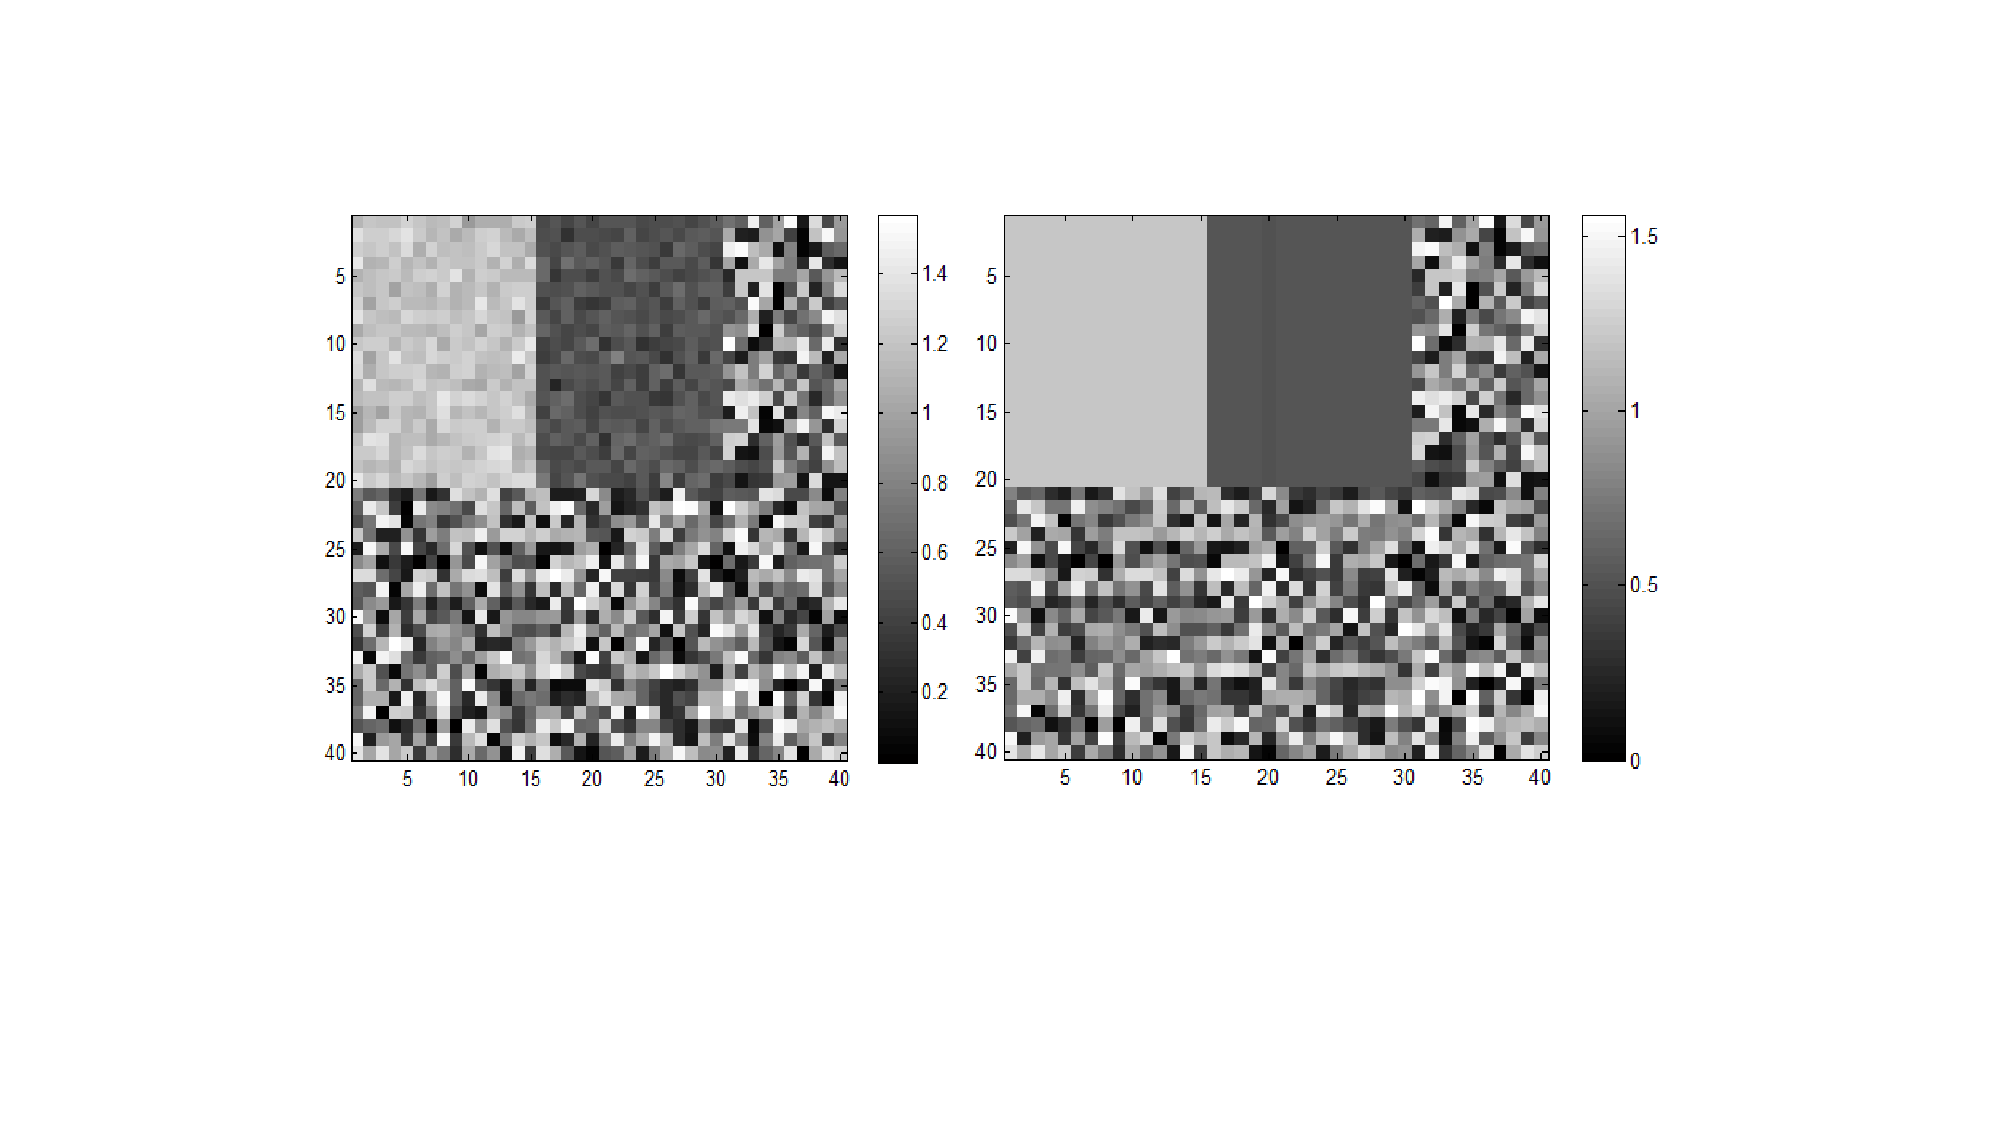
\includegraphics[width=140mm]{ap3}
\caption {双联合簇,并排分布}
\label{fig:idea}
\end{figure}

\begin{figure}
\centering
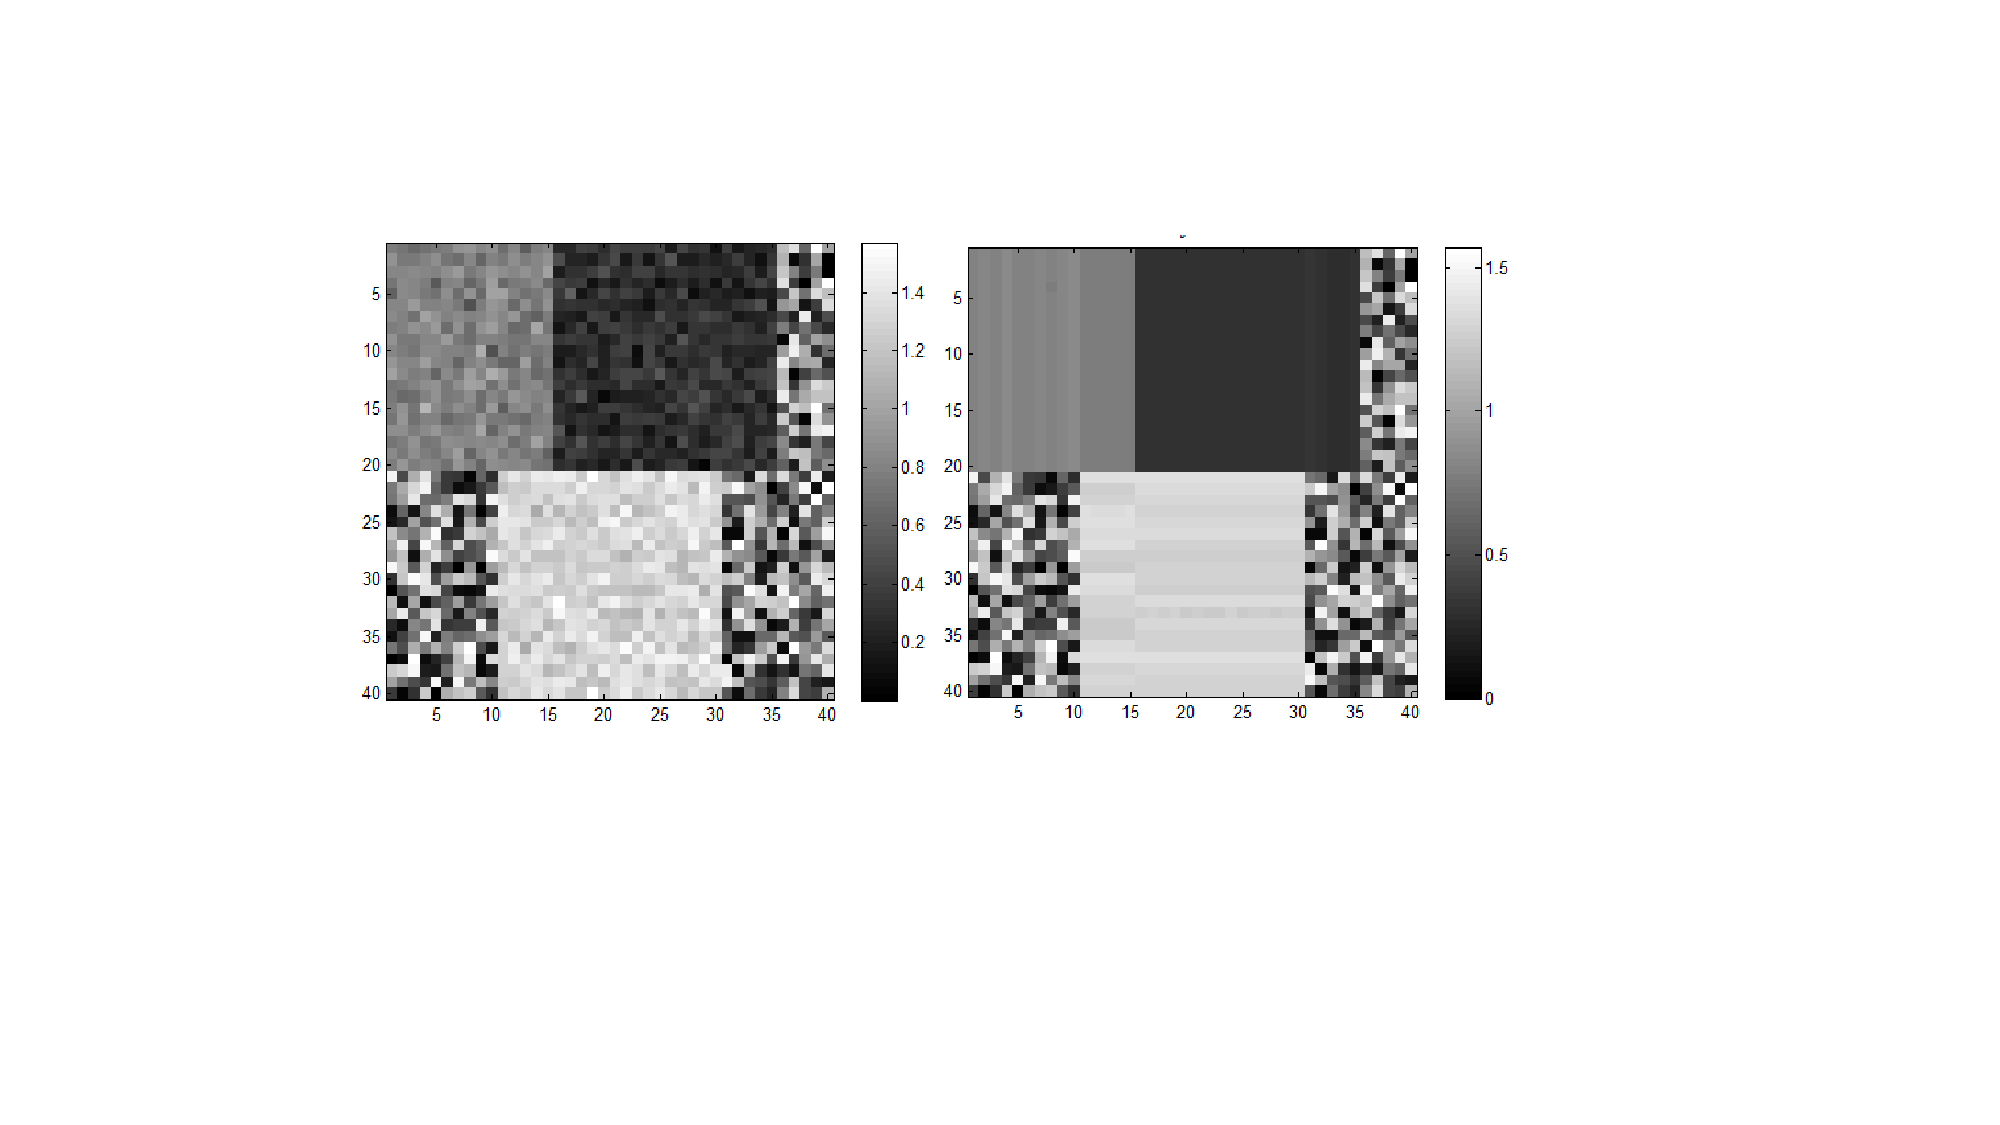
\includegraphics[width=140mm]{ap4}
\caption {三联合簇,不规则分布}
\label{fig:idea}
\end{figure}

\begin{figure}
\centering
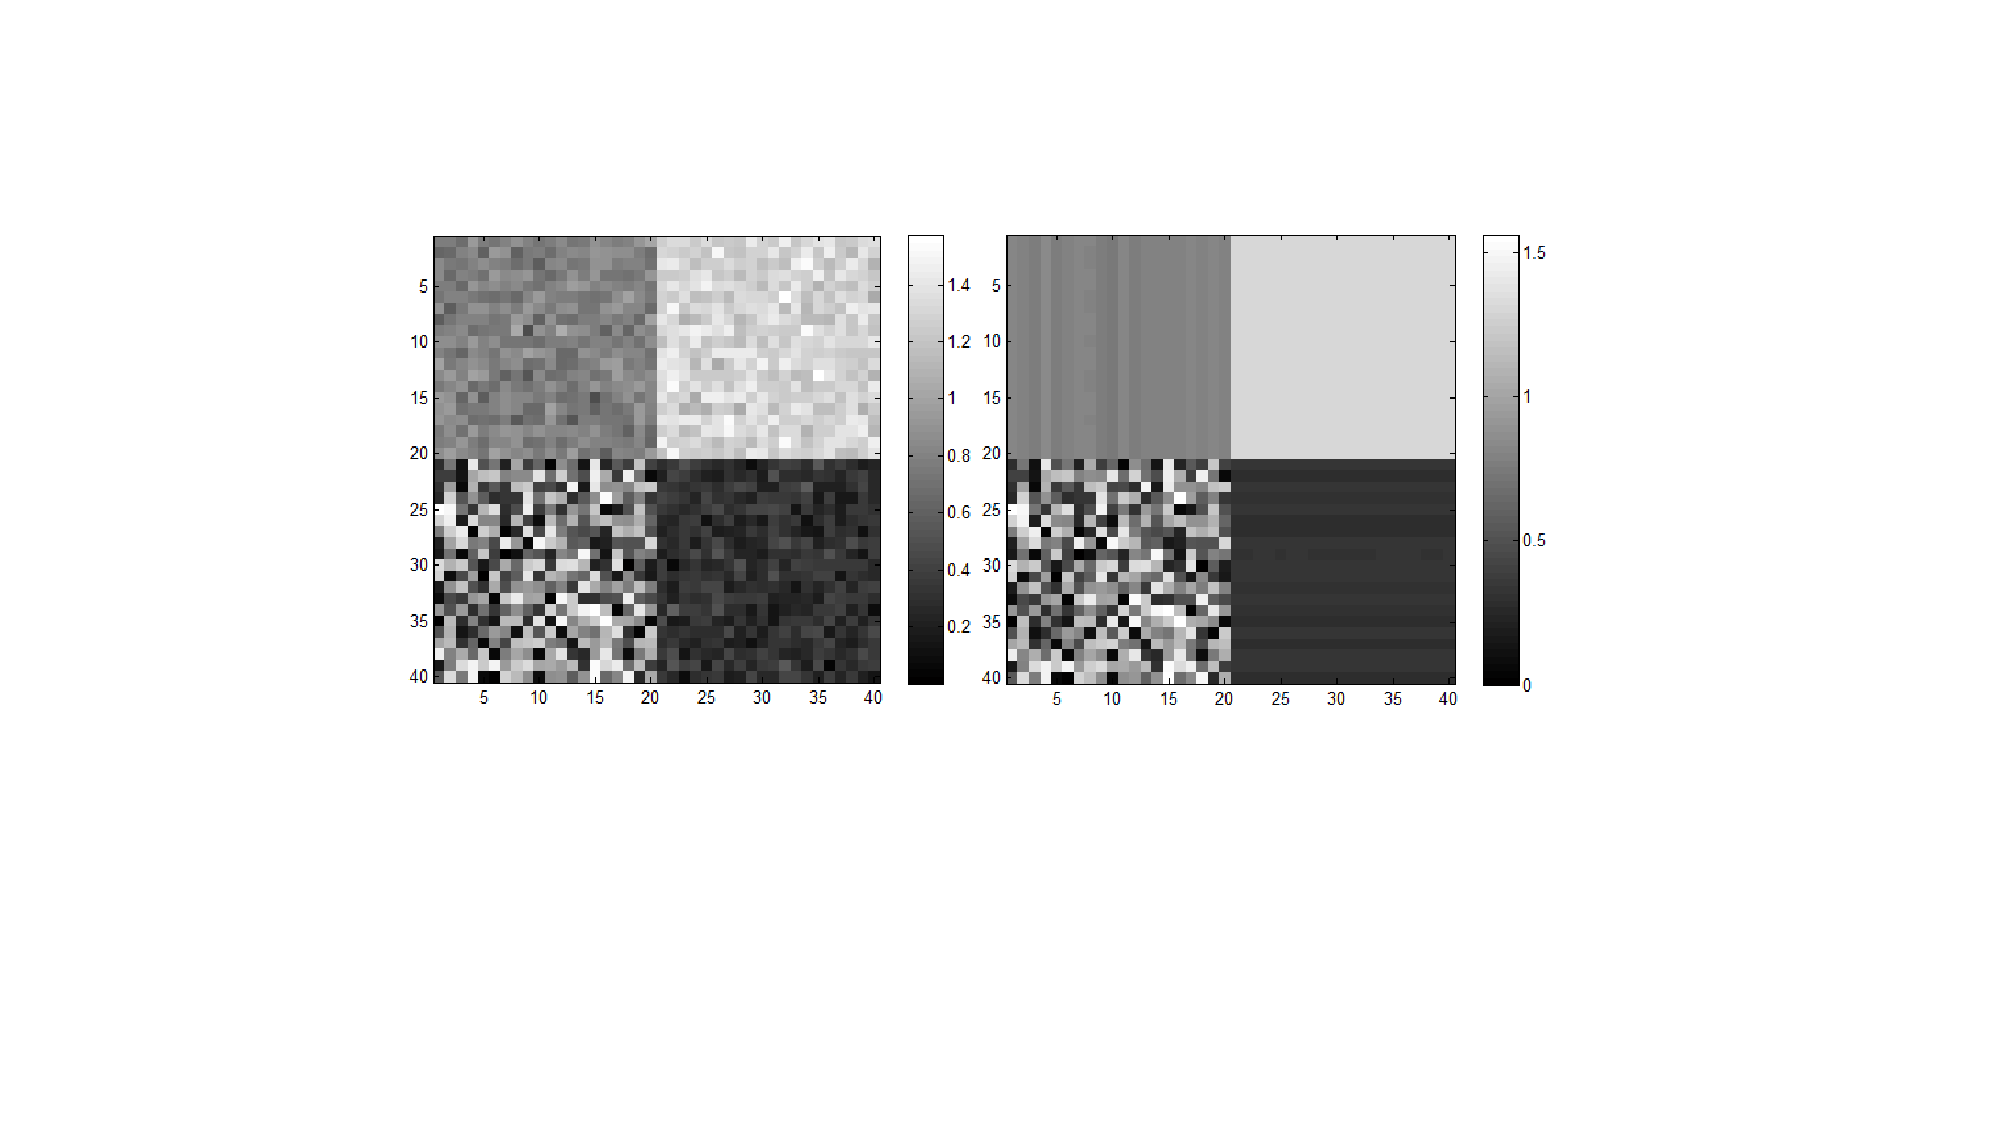
\includegraphics[width=140mm]{ap5}
\caption {三联合簇,规则分布}
\label{fig:idea}
\end{figure}

% \vspace{-8mm}
% \pic[!htb]{双联合簇,并排分布}{width=140mm}{ap3}
% \vspace{-4mm}
% \pic[!htb]{三联合簇,不规则分布}{width=140mm}{ap4}
% \vspace{-4mm}
% \pic[!hb]{三联合簇,规则分布}{width=140mm}{ap5}
% \vspace{-4mm}
%插入附录内容
\clearpage
%    \end{macrocode}
% \subsubsection{本科外文资料翻译章节特殊设置}
% \changes{v0.4.5}{2013/06/01}{设置外文资料章节的特殊格式。改写标准章节命令,让它们不向目录中加入条目。并重置章节号。}
% 下面第一行先判断是否为本科论文。由于有的同学需要在外文翻译这两部分中使用章节标题命令。而又不希望它们按照正文的形式显示在目录中,所以需要如下设置。
%    \begin{macrocode}
\ifdefstring{\degree@uestcthesis}{bachelor}{

\gdef\thechapter{\@arabic \c@chapter}
%将章号由附录的ABC形式改回123形式.

\CTEXsetup[ name={,},
  number={}
  ]{chapter}
%去掉|\chapter|命令生成的章标题章号。

\setcounter{chapter}{0}
%让节标题使用的章号重新从1开始。形成1.1,1.2的节标题结构。

\def\Hy@org@chapter[#1]#2{%
\ifnum \c@secnumdepth >\m@ne \if@mainmatter \refstepcounter {chapter}
\typeout {\CTEXthechapter }\else \fi \else \fi \chaptermark {#1}\addtocontents{lof}
{\protect \addvspace {10\p@ }}\addtocontents {lot}{\protect \addvspace {10\p@ }}
\if@twocolumn \@topnewpage [\@makechapterhead {#2}]
\else
\@makechapterhead {#2}
\@afterheading \fi
}
%去掉|\chapter|命令中的自动向目录中加入条目的功能。之后再使用|\chapter|命令,目录中不会产生新条目了。

\def\H@old@sect #1#2#3#4#5#6[#7]#8{\ifnum #2>\c@secnumdepth \let \@svsec \@empty
\else \refstepcounter {#1}\protected@edef \@svsec {\@seccntformat {#1}\relax }\fi
\@tempskipa #5\relax \ifdim \@tempskipa >\z@ \begingroup #6{\@hangfrom {\hskip #3
\relax \@svsec }\interlinepenalty \@M \csname CTEX@#1@titleformat\endcsname #8
\@@par }\endgroup \csname #1mark\endcsname {#7}\else \def \@svsechd
 {#6{\hskip #3\relax \@svsec \csname CTEX@#1@titleformat\endcsname #8}\csname #1mark
 \endcsname {#7}}\fi \@xsect {#5}}
%去掉所有节标题命令自动向目录中加入条目的功能。之后使用|\section\subsection|等命令不会向目录中加入新条目了。



\renewcommand{\chaptermark}[1]{\markboth{外文资料原文}{}}
\def\leftmark{外文资料原文}
\newpage
\phantomsection
\addcontentsline{toc}{chapter}{外文资料原文}

\renewcommand{\CTEX@figurename}{Figure}
\renewcommand{\CTEX@tablename}{Table}
%在外文资料中图表题注使用英文显示。

% !Mode:: "TeX:UTF-8"

% \chapter{The Name of the Game}
% \section{xxx}
% \subsection{xxx}
% \subsubsection{xxxx}
% \section{xxx}
% \subsection{xxx}
% \subsubsection{xxxx}
% English words like `technology' stem from a Greek root beginning with
% the letters $\tau\epsilon\chi\ldots\,$; and this same Greek word means {\sl
% art\/} as well as technology. Hence the name \TeX, which is an
% uppercase form of $\tau\epsilon\chi$.{TeX (actually \TeX), meaning of}
% $\tau\epsilon\chi$

% Insiders pronounce the $\chi$ of \TeX\ as a Greek chi, not as an `x', so that
% \TeX\ rhymes with the word blecchhh. It's the `ch' sound in Scottish words
% like {\sl loch\/} or German words like {\sl ach\/}; it's a Spanish `j' and a
% Russian `kh'. When you say it correctly to your computer, the terminal
% may become slightly moist.

% The purpose of this pronunciation exercise is to remind you that \TeX\ is
% primarily concerned with high-quality technical manuscripts: Its emphasis is
% on art and technology, as in the underlying Greek word. If you merely want
% to produce a passably good document---something acceptable and basically
% readable but not really beautiful---a simpler system will usually suffice.
% With \TeX\ the goal is to produce the {\sl finest\/} quality; this requires
% more attention to detail, but you will not find it much harder to go the
% extra distance, and you'll be able to take special pride in the finished
% product.

% On the other hand, it's important to notice another thing about \TeX's name:
% The `E' is out of kilter. This {logo}
% displaced `E' is a reminder that \TeX\ is about typesetting, and it
% distinguishes \TeX\ from other system names. In fact, {TEX} (pronounced
% {\sl tecks\/}) is the admirable {\sl Text EXecutive\/} processor developed by
% {Honeywell Information Systems}. Since these two system names are
% {Bemer, Robert, see TEX, ASCII}
% pronounced quite differently, they should also be spelled differently. The
% correct way to refer to \TeX\ in a computer file, or when using some other
% medium that doesn't allow lowering of the `E', is to type `|TeX|'. Then
% there will be no confusion with similar names, and people will be
% primed to pronounce everything properly.

\newpage
\phantomsection
\addcontentsline{toc}{chapter}{外文资料译文}
\renewcommand{\chaptermark}[1]{\markboth{外文资料译文}{}}
\def\leftmark{外文资料译文}

\renewcommand{\CTEX@figurename}{图}
\renewcommand{\CTEX@tablename}{表}
%将图表题注由英文改回中文。

\setcounter{chapter}{0}
%由于译文和原文是对照翻译的形式,所以章号依然重置为1。

% !Mode:: "TeX:UTF-8"


}
%    \end{macrocode}
% \subsubsection{硕博攻读期间发表论文章节特殊设置}
% 下面的大括号实际上是上一节判断是否为本科论文的|\ifdefstring|命令的else部分。也就是只有硕博论文才执行的命令。
%    \begin{macrocode}
{
\ifdef{\usecv@uestcthesis}{\usecv@uestcthesis}{
	\IfFileExists{contents/publications.bib}{%如果删除了publications.bib,则不显示这一章
	\CTEXoptions[ bibname={\publicationsname@degree}]%设置攻博/硕期间发表的论文章题目
	\phantomsection%手动添加目录项之前需要这个命令,用以更新目录超链接的跳转页码。
	\addcontentsline{toc}{chapter}{\publicationsname@degree}%将攻博/硕期间发表的论文编入目录
	{\zihao{5}\baselineskip=20bp{}%
%    \end{macrocode}
% footmisc宏包的perpage选项会向每个aux文件中写入一个命令。由于publications没有tex文件,只有aux文件。所以出现了错误。这里将要写入aux文件的内容清空。
%    \begin{macrocode}
	\def\footnotehint{}%
	\bibliographypublications{contents/publications}%插入攻博/硕期间发表的论文
	}}{}
	}
}
\clearpage\end{CJK}}
}%这是大括号是前面onlychapters选项的ifdef命令的一部分。
%    \end{macrocode}
% \iffalse
%</class>
% \fi
% \iffalse
%<*bst>
% \fi
% \section{参考文献样式}
% \changes{v0.3}{2013/2/12}{修复了参考文献模板bst文件中原有的问题,
% 不再需要其他工具替换bbl中的错误。即参考文献中的“|\\.|”修正为“|\\|”。}
% \changes{v0.4.4}{2013/05/23}{增加一个参考文献类型,主要用于在攻读期间取得成果
% 内录入获奖等不符合参考文献规范的内容。}
% \changes{v1.2.0}{2015/04/08}{将uestcthesis.bst模板中原有的参考文献类型全部删除。重新定义了9个参考文献类型,分别对应研究生院规范中的9种参考文献类型。另外,OnlyNote类型保留下来了。}
%\changes{v1.2.2}{2015/04/23}{修正参考文献的悬挂缩进对齐。强制参考文献标题只有第一个字母大写。}
%%本文件基于吴凯制作的GBT7714-2005NLang.bst(1 Beta 2 测试版2012年9月20日)修改而成。
%%修改内容包括将英文作者的名放前姓放后,设置行距。删除原有的参考文献类型,重新定义了10个参考文献类型。使用方法需要参考本模板的WIKI。
%%根据GBT7714-2005NLang.bst中copyright的要求,将文件名修改成uestcthesis.bst。
%%对吴凯的杰出工作表示感谢!
%bst文件内容不在文档中显示。
% \iffalse
ENTRY
  { address
    author
    booktitle
    chapter
    edition
    editor
    howpublished
    institution
    journal
    key
    month
    note
    number
    organization
    pages
    publisher
    school
    series
    title
    type
    volume
    year
    url
    TypeofLit                %新加入:文献类型和标志代码
    normalauthor             %不改变大小写的作者
    normaleditor             %不改变大小写的编者
    translator               %新加入:翻译者
    date                     %日期,公告日期,公开日期
    modifydate               %修改日期
    citedate                 %引用日期
    patentid                 %专利号
    country                  %国家(主要用于专利中)
    miscyear                 %其它类中用于输出年份
    startyear                %起始年
    startvolume              %起始卷
    startnumber              %起始期
    endyear                  %终止年
    endvolume                %终止卷
    endnumber                %终止期
    language                 %默认是英文文献,非空则表明是中文文献
  }
  {}
  { label extra.label sort.label short.list }

INTEGERS { output.state before.all mid.sentence after.sentence after.block }
FUNCTION {format.url}
{ url empty$
    { "" }
    { new.block
    "\url{" url * "}" * }
  if$
}
FUNCTION {init.state.consts}
{ #0 'before.all :=
  #1 'mid.sentence :=
  #2 'after.sentence :=
  #3 'after.block :=
}

STRINGS { s t }

FUNCTION {output.nonnull}
{ 's :=
  output.state mid.sentence =
    { ", " * write$ }
    { output.state after.block =
    { add.period$ write$
      newline$
      "\newblock " write$
    }
    { output.state before.all =
        'write$
        { add.period$ " " * write$ }
      if$
    }
      if$
      mid.sentence 'output.state :=
    }
  if$
  s
}

FUNCTION {coutput.nonnull}                                   %wk
{ 's :=
  output.state mid.sentence =
    { "," * write$ }                                       %
    { output.state after.block =
    { add.period$ write$
      newline$
      "\newblock " write$
    }
    { output.state before.all =
        'write$
        { add.period$ " " * write$ }
      if$
    }
      if$
      mid.sentence 'output.state :=
    }
  if$
  s
}

FUNCTION {output}
{ duplicate$ empty$
    'pop$
    'output.nonnull
  if$
}

FUNCTION {coutput}                                           %wk
{ duplicate$ empty$
    'pop$
    'coutput.nonnull
  if$
}

FUNCTION {output.check}
{ 't :=
  duplicate$ empty$
    { pop$ "empty " t * " in " * cite$ * warning$ }
    'output.nonnull
  if$
}

FUNCTION {coutput.check}                                     %wk
{ 't :=
  duplicate$ empty$
    { pop$ "empty " t * " in " * cite$ * warning$ }
    'coutput.nonnull
  if$
}

FUNCTION {output.year.month.check}
{ year empty$
    { "empty year in " cite$ * warning$ }
    { add.period$ write$
      month empty$
        { " " year * extra.label * "." *
          after.sentence 'output.state :=
        }
        { " " year * extra.label * " (" * month * ")." *
          after.sentence 'output.state :=
        }
      if$
    }
  if$
}

FUNCTION {output.cyear.month.check}                            %wk
{ year empty$
    { "empty year in " cite$ * warning$ }
    {write$
      month empty$
        {year                      %wk
          after.sentence 'output.state :=
        }
        { "" year * extra.label * "(" * month * ")" *     %wk
          after.sentence 'output.state :=
        }
      if$
    }
  if$
}

%%%%%%%%%%%%%%%%%%%%%%%%%%%%%%%%%%%%%%%%%%%%%%%%%%%%%%%%%%%%%%%%%%%%%%%%%%%%%%%%
FUNCTION {output.modifydate.check}
{modifydate
}

FUNCTION {output.citedate.check}
{ year empty$
    { "" }
    { write$
      "[" citedate * extra.label * "]" *
      after.sentence 'output.state :=
    }
  if$
}

FUNCTION {output.year.check}
{ year empty$
    { "empty year in " cite$ * warning$ }
    {miscyear empty$
        {year}
         {miscyear}
     if$                     %wk
    }
  if$
  extra.label *
}

FUNCTION {output.cyear.check}                           %wk
{ year empty$
    { "empty year in " cite$ * warning$ }
    {miscyear empty$
        {year}
         {miscyear}
     if$                     %wk
    }
  if$
  extra.label *
}
%%%%%%%%%%%%%%%%%%%%%%%%%%%%%%%%%%%%%%%%%%%%%%%%%%%%%%%%%%%%%%%%%%%%%%%

FUNCTION {output.continue.year.check}                           %wk
{
endyear empty$
   {startyear empty$
      {year empty$
         { "empty year in " cite$ * warning$ }
         {"" year * "" * }
       if$
       }
      {"" startyear * "-" * }
    if$
    }
{startyear empty$
    {year empty$
        { "empty year in " cite$ * warning$ }
        {"" year * "" * }
    if$
    }
    {"" startyear * "-" *
    "" endyear * "" * *
    }
 if$
}
if$
}

FUNCTION {output.continue.cyear.check}                           %wk
{
endyear empty$
   {startyear empty$
      {year empty$
         { "empty year in " cite$ * warning$ }
         {"" year * "" * }
       if$
       }
      {"" startyear * "-" * }
    if$
    }
{startyear empty$
    {year empty$
        { "empty year in " cite$ * warning$ }
        {"" year * "" * }
    if$
    }
    {"" startyear * "-" *
    "" endyear * "" * *
    }
 if$
}
if$
}

%%%%%%%%%%%%%%%%%%%%%%%%%%%%%%%%%%%%%%
FUNCTION {output.article.year.check}
{month empty$
{
year empty$
    { "empty year in " cite$ * warning$ }
    {year                 %wk
    }
  if$
}
{
TypeofLit empty$
       {year empty$
    { "empty year in " cite$ * warning$ }
    {year                 %wk
    }
  if$}

{year empty$
    { "empty year in " cite$ * warning$ }
    {year                 %wk
       "-"  month * "" * *
    }
  if$
}
if$
}
if$
}

FUNCTION {output.carticle.year.check}                           %wk
{month empty$
{
year empty$
    { "empty year in " cite$ * warning$ }
    {year                 %wk
    }
  if$
}
{
TypeofLit empty$
       {year empty$
    { "empty year in " cite$ * warning$ }
    {year                 %wk
    }
  if$}

{year empty$
    { "empty year in " cite$ * warning$ }
    {year                 %wk
       "-"  month * "" * *
    }
  if$
}
if$
}
if$
}
%%%%%%%%%%%%%%%%%%%%%%%%%%%%%%%%%%%%%%

FUNCTION {output.bibitem}
{ newline$
  "\ifnum \value{NAT@ctr}=9 \addtolength{\labelwidth}{1em} \fi" write$
  "\ifnum \value{NAT@ctr}=99 \addtolength{\labelwidth}{1em} \fi" write$
  "\ifnum \value{NAT@ctr}=999 \addtolength{\labelwidth}{1em} \fi" write$
  "\bibitem[" write$
  label write$
  "]{" write$
  cite$ write$
  "}" write$
  newline$
  ""
  before.all 'output.state :=
}

FUNCTION {fin.entry}
{ write$
  newline$
}

FUNCTION {new.block}
{ output.state before.all =
    'skip$
    { after.block 'output.state := }
  if$
}

FUNCTION {new.sentence}
{ output.state after.block =
    'skip$
    { output.state before.all =
        'skip$
        { after.sentence 'output.state := }
      if$
    }
  if$
}

FUNCTION {not}
{   { #0 }
    { #1 }
  if$
}

FUNCTION {and}
{   'skip$
    { pop$ #0 }
  if$
}

FUNCTION {or}
{   { pop$ #1 }
    'skip$
  if$
}

FUNCTION {new.block.checkb}
{ empty$
  swap$ empty$
  and
    'skip$
    'new.block
  if$
}

FUNCTION {field.or.null}
{ duplicate$ empty$
    { pop$ "" }
    'skip$
  if$
}

FUNCTION {boldface}
{ duplicate$ empty$
    { pop$ "" }
    { "{\bf " swap$ * "}" * }
  if$
}


%%%%%%%%%%%%%%%%%%%
Function{upcase}
{ duplicate$ empty$
    { pop$ "" }
    { "u" change.case$ }
  if$
}
%%%%%%%%%%%%%%%%%%%%

%%%%%%%%%%%%%%%%%%%%%%%

INTEGERS { nameptr namesleft numnames }

FUNCTION {capitalize}
{ "u" change.case$ "t" change.case$ }

FUNCTION {format.names}
{ 's :=
  #1 'nameptr :=
  s num.names$ 'numnames :=
  numnames 'namesleft :=
    { namesleft #0 > }
    { s nameptr "{f.~}{vv~}{ll}{, jj}"
    format.name$
    remove.dots
     't :=
      nameptr #1 >
        {
          nameptr #3
          #1 + =
          numnames #3
          > and
            { "others" 't :=
              #1 'namesleft := }
            'skip$
          if$
          namesleft #1 >
            { ", " * t * }
            { numnames #2 >
              { "" * }
              'skip$
              if$
              s nameptr "{ll}" format.name$ duplicate$ "others" =
                { 't := }
                { pop$ }
              if$
              t "others" =
                 {%bib.name.font    %改为大写
                  ", et al" *
                }
                {", " * t * }
              if$
            }
          if$
        }
        't
      if$
      nameptr #1 + 'nameptr :=
      namesleft #1 - 'namesleft :=
    }
  while$
%%%%%%%%%%%
%%%%%%%%%%%
}

FUNCTION {format.cnames}                                     %wk
{ 's :=
  #1 'nameptr :=
  s num.names$ 'numnames :=
  numnames 'namesleft :=
    { namesleft #0 > }
    { s nameptr "{vv~}{ll}{ f{~}}{ jj}" format.name$
    remove.dots
    't :=
      nameptr #1 >
        {
          nameptr #3
          #1 + =
          numnames #3
          > and
            { "others" 't :=
              #1 'namesleft := }
            'skip$
          if$
          namesleft #1 >
            { ", " * t * }
            { numnames #2 >
              { "" * }
              'skip$
              if$
              s nameptr "{ll}" format.name$ duplicate$ "others" =
                { 't := }
                { pop$ }
              if$
              t "others" =
                 { ",等" *
               % bib.name.font    %改为大写
                }
                {", " * t * }
              if$
            }
          if$
        }
        't
      if$
      nameptr #1 + 'nameptr :=
      namesleft #1 - 'namesleft :=
    }
  while$
%%%%%%%%%%%
%%%%%%%%%%%
}

%%%%%%%%%%%%%%%%%%%%%%%%%%%%%%%%%%%%%%%%%%%%%%%%%%%%%%%%%%%%%%%%%%%%%%%
%%%%%%%%%%%%%%%%%%%%%%%%%%%%%%%%%%%%%%%%%%%%%%%%%%%%%%%%%%%%%%%%%%%%%%%

FUNCTION {format.normal.names}
{ 's :=
  #1 'nameptr :=
  s num.names$ 'numnames :=
  numnames 'namesleft :=
    { namesleft #0 > }
    { s nameptr "{vv~}{ll}{ f{~}}{, jj}"
    format.name$
    remove.dots
     't :=
      nameptr #1 >
        {
          nameptr #3
          #1 + =
          numnames #3
          > and
            { "others" 't :=
              #1 'namesleft := }
            'skip$
          if$
          namesleft #1 >
            { ", " * t * }
            { numnames #2 >
              { "" * }
              'skip$
              if$
              s nameptr "{ll}" format.name$ duplicate$ "others" =
                { 't := }
                { pop$ }
              if$
              t "others" =
                 { ", et al" * }
                {", " * t * }
              if$
            }
          if$
        }
        't
      if$
      nameptr #1 + 'nameptr :=
      namesleft #1 - 'namesleft :=
    }
  while$
}

FUNCTION {format.normal.cnames}                                    %wk
{ 's :=
  #1 'nameptr :=
  s num.names$ 'numnames :=
  numnames 'namesleft :=
    { namesleft #0 > }
    { s nameptr "{vv~}{ll}{ f{~}}{ jj}" format.name$
    remove.dots
    't :=
      nameptr #1 >
        {
          nameptr #3
          #1 + =
          numnames #3
          > and
            { "others" 't :=
              #1 'namesleft := }
            'skip$
          if$
          namesleft #1 >
            { ", " * t * }
            { numnames #2 >
              { "" * }
              'skip$
              if$
              s nameptr "{ll}" format.name$ duplicate$ "others" =
                { 't := }
                { pop$ }
              if$
              t "others" =
                 { ",等" * }
                {", " * t * }
              if$
            }
          if$
        }
        't
      if$
      nameptr #1 + 'nameptr :=
      namesleft #1 - 'namesleft :=
    }
  while$
}
%%%%%%%%%%%%%%%%%%%%%%%%%%%%%%%%%%%%%%%%%%%%%%%%%%%%%%%%%%%%%%%%%%%%%%

FUNCTION {format.authors}
{ author empty$
    { "" }
    {normalauthor empty$
         {author format.names }
         {normalauthor format.normal.names}
    if$
}
  if$
}

FUNCTION {format.cauthors}                                   %wk
{ author empty$
    { "" }
    {normalauthor empty$
         {author format.cnames }
         {normalauthor format.normal.cnames}
    if$
}
  if$
}

FUNCTION {format.key}
{ empty$
    { key field.or.null }
    { "" }
  if$
}

FUNCTION {format.editors}
{ editor empty$
    { "" }
    {normaleditor empty$
         {editor format.names }
         {normaleditor format.normal.names}
    if$
      editor num.names$ #1 >                                %  Use ODWE abbrevs.
        { "" * }                                      %  to avoid
        { "" * }                                       %  ambiguity between
      if$                                                   %  "editor" and
    }                                                       %  "edition".
  if$
}

FUNCTION {format.ceditors}                                 %wk   本函数
{ editor empty$
    { "" }
    {
    normaleditor empty$
         {editor * "" * format.cnames }
         {normaleditor * "" * format.normal.cnames}
    if$
    }
  if$
}
%%%%%%%%%%%%%%%%%%%%%%%%%%%%%%%%%%%%%%%%
FUNCTION {format.title}                                     %  Nothing needs
{ title empty$                                              %  doing here in
    { "" }                                                  %  authordate1.bst
    { title }                                               %  or
  if$                                                       %  authordate3.bst.
}

FUNCTION {format.ctitle}                %wk                 %  Nothing needs
{ title empty$                                              %  doing here in
    { "" }                                                  %  authordate1.bst
    {title}                                               %  or
  if$                                                       %  authordate3.bst.
}
%%%%%%%%%%%%%%%%%%%%%%%%%%%%%%%%%%%%%%%%%%%%%%%%%%%%%

FUNCTION {format.article.title}                                     %  Nothing needs
{title empty$                                              %  doing here in
    { "" }                                                  %  authordate1.bst
    {
    typeoflit empty$
       {format.title "[J]" * title output.check}
       {format.title title output.check}
    if$
    }
if$
TypeofLit empty$
       {""}
       { "["  TypeofLit * "]" * * }
if$
                                                    %  authordate3.bst.
}

FUNCTION {format.carticle.title}                                     %  Nothing needs
{title empty$                                              %  doing here in
    { "" }                                                  %  authordate1.bst
    {
    typeoflit empty$
       {format.title "[J]" * title output.check}
       {format.title title output.check}
    if$
    }
if$

TypeofLit empty$
       {""}
       { "[" TypeofLit * "]" * *  }
if$
                                                     %  authordate3.bst.
}
%%%%%%%%%%%%%%%%%%%%%%%%%%%%%%%%%%%%%%%%
FUNCTION {format.book.title}                                     %  Nothing needs
{title empty$                                              %  doing here in
    { "" }                                                  %  authordate1.bst
    {
    typeoflit empty$
       {format.title "[M]" * title output.check}
       {format.title title output.check}
    if$
    }
if$
TypeofLit empty$
       {""}
       { "["  TypeofLit * "]" * * }
if$
                                                    %  authordate3.bst.
}

FUNCTION {format.cbook.title}                %wk                 %  Nothing needs
{title empty$                                              %  doing here in
    { "" }                                                  %  authordate1.bst
    {
    typeoflit empty$
       {format.title "[M]" * title output.check}
       {format.title title output.check}
    if$
    }
if$
TypeofLit empty$
       {""}
       { "["  TypeofLit * "]" * * }
if$
                                                    %  authordate3.bst.
}
%%%%%%%%%%%%%%%%%%%%%%%%%%%%%%%%%%%%%%%%%%%%%%%%%%%%%
FUNCTION {format.misc.title}                %wk                 %  Nothing needs
{
patentid empty$
       {%没有专利号应该是其它类型文献,直接标准输出
title empty$                                              %  doing here in
    { "" }                                                  %  authordate1.bst
    {
    typeoflit empty$
       {format.title "[缺文献类型标志代码]." * title output.check}
       {format.title title output.check}
    if$
    }
if$
TypeofLit empty$
       {""}
       { "["  TypeofLit * "]." * * }
if$
       }
       {%有专利号
          country empty$
             {
title empty$                                              %  doing here in
    { "" }                                                  %  authordate1.bst
    {
    typeoflit empty$
       {format.title "[缺文献类型标志代码]." * title output.check}
       {format.title title output.check}
    if$
    }
if$
TypeofLit empty$
       {""}
       { "["  TypeofLit * "]." * * }
if$
""  patentid * "" * *
             }
             {%有专利号,有国家
title empty$                                              %  doing here in
    { "" }                                                  %  authordate1.bst
    {
    typeoflit empty$
       {format.title "[缺文献类型标志代码]." * title output.check}
       {format.title title output.check}
    if$
    }
if$

              ":"  country * "," * *
              ""  patentid * "" * *
TypeofLit empty$
       {""}
       { "["  TypeofLit * "]." * * }
if$

              }
             if$
}
if$

}

FUNCTION {format.cmisc.title}                %wk                 %  Nothing needs
{
patentid empty$
       {%没有专利号应该是其它类型文献,直接标准输出
title empty$                                              %  doing here in
    { "" }                                                  %  authordate1.bst
    {
    typeoflit empty$
       {format.title "[缺文献类型标志代码]." * title output.check}
       {format.title title output.check}
    if$
    }
if$
TypeofLit empty$
       {""}
       { "["  TypeofLit * "]." * * }
if$
       }
       {%有专利号
          country empty$
             {
title empty$                                              %  doing here in
    { "" }                                                  %  authordate1.bst
    {
    typeoflit empty$
       {format.title "[缺文献类型标志代码]." * title output.check}
       {format.title title output.check}
    if$
    }
if$
TypeofLit empty$
       {""}
       { "["  TypeofLit * "]." * * }
if$
""  patentid * "" * *
             }
             {%有专利号,有国家
title empty$                                              %  doing here in
    { "" }                                                  %  authordate1.bst
    {
    typeoflit empty$
       {format.title "[缺文献类型标志代码]." * title output.check}
       {format.title title output.check}
    if$
    }
if$

              ":"  country * "," * *
              ""  patentid * "" * *
TypeofLit empty$
       {""}
       { "["  TypeofLit * "]." * * }
if$

              }
             if$
}
if$

}
%%%%%%%%%%%%%%%%%%%%%%%%%%%%%%%%%%%%%%%%%%%%%%%%%%%%%

%%%%%%%%%%%%%%%%%%%%%%%%%%%%%%%%%%%%%%%%%%%%%%%%%%%%%%

FUNCTION {format.proceedings.title}                                     %  Nothing needs
{title empty$                                              %  doing here in
    { "" }                                                  %  authordate1.bst
    {
    typeoflit empty$
       {format.title "[C]" * title output.check}
       {format.title title output.check}
    if$
    }
if$

TypeofLit empty$
       {""}
       { "[" TypeofLit * "]" * *  }
if$
                                                     %  authordate3.bst.
}

FUNCTION {format.cproceedings.title}                                     %  Nothing needs
{title empty$                                              %  doing here in
    { "" }                                                  %  authordate1.bst
    {
    typeoflit empty$
       {format.title "[C]" * title output.check}
       {format.title title output.check}
    if$
    }
if$

TypeofLit empty$
       {""}
       { "[" TypeofLit * "]" * *  }
if$
                                                     %  authordate3.bst.
}
%%%%%%%%%%%%%%%%%%%%%%%%%%%%%%%%%%%%%%%%%%%%%%%%
FUNCTION {format.incollection.title}                                     %  Nothing needs
{title empty$                                              %  doing here in
    { "" }                                                  %  authordate1.bst
    {
    typeoflit empty$
       {format.title "[M]//" * title output.check}
       {format.title "" * title output.check}
    if$
    }
if$

TypeofLit empty$
       {""}
       { "[" TypeofLit * "]//" * * }
if$
                                                     %  authordate3.bst.
}

FUNCTION {format.cincollection.title}                                     %  Nothing needs
{title empty$                                              %  doing here in
    { "" }                                                  %  authordate1.bst
    {
    typeoflit empty$
       {format.title "[M]//" * title output.check}
       {format.title "" * title output.check}
    if$
    }
if$

TypeofLit empty$
       {""}
       { "[" TypeofLit * "]//" * * }
if$
                                                     %  authordate3.bst.
}
%%%%%%%%%%%%%%%%%%%%%%%%%%%%%
FUNCTION {format.inproceedings.title}                                     %  Nothing needs
{title empty$                                              %  doing here in
    { "" }                                                  %  authordate1.bst
    {
    typeoflit empty$
       {format.title "[C]//" * title output.check}
       {format.title "" * title output.check}
    if$
    }
if$

TypeofLit empty$
       {""}
       { "[" TypeofLit * "]//" * * }
if$
                                                     %  authordate3.bst.
}

FUNCTION {format.cinproceedings.title}                                     %  Nothing needs
{title empty$                                              %  doing here in
    { "" }                                                  %  authordate1.bst
    {
    typeoflit empty$
       {format.title "[C]//" * title output.check}
       {format.title "" * title output.check}
    if$
    }
if$

TypeofLit empty$
       {""}
       { "[" TypeofLit * "]//" * * }
if$
                                                     %  authordate3.bst.
}
%%%%%%%%%%%%%%%%%%%%%%%%%%%%%

FUNCTION {n.dashify}
{ 't :=
  ""
    { t empty$ not }
    { t #1 #1 substring$ "-" =
        { t #1 #2 substring$ "--" = not
            { "--" *
              t #2 global.max$ substring$ 't :=
            }
            {   { t #1 #1 substring$ "-" = }
               { "-" *
                 t #2 global.max$ substring$ 't :=
               }
              while$
            }
          if$
        }
        { t #1 #1 substring$ *
          t #2 global.max$ substring$ 't :=
        }
        if$
    }
  while$
}

FUNCTION {format.btitle}
{ title empty$
   { "" }                                                   %  Don't change case
   {booktitle}                                      %  in
   if$                                                      %  authordate1.bst
}                                                           %  or

FUNCTION {format.cbtitle}                  %wk                 %  Nothing needs
{ title empty$                                              %  doing here in
    { "" }                                                  %  authordate1.bst
    {booktitle}                                               %  or
  if$                                                       %  authordate3.bst.
}
                                                            %  authordate3.bst.
FUNCTION {tie.or.space.connect}
{ duplicate$ text.length$ #3 <
    { "~" }
    { " " }
  if$
  swap$ * *
}

FUNCTION {either.or.check}
{ empty$
    'pop$
    { "can't use both " swap$ * " fields in " * cite$ * warning$ }
  if$
}

INTEGERS { multiresult }

FUNCTION {multi.page.check}
{ 't :=
  #0 'multiresult :=
    { multiresult not
      t empty$ not
      and
    }
    { t #1 #1 substring$
      duplicate$ "-" =
      swap$ duplicate$ "," =
      swap$ "+" =
      or or
        { #1 'multiresult := }
        { t #2 global.max$ substring$ 't := }
      if$
    }
  while$
  multiresult
}

FUNCTION {format.numberinseries}
{ number empty$
    { "" }
    { number multi.page.check
        { ", nos. " number n.dashify tie.or.space.connect }
        { ", no. "  number tie.or.space.connect }
      if$
    }
  if$
}

FUNCTION {format.cnumberinseries}                           %wk
{ number empty$
    { "" }
    { number multi.page.check
        { ", 第" number n.dashify tie.or.space.connect * "期"}  %wk
        { ", 第"  number tie.or.space.connect * "期"}           %wk
      if$
    }
  if$
}
%%%%%%%%%%%%%%%%%%%%%%%%%%%%%%%%%%%%%%%%%%%
FUNCTION {booklike.series.volume.number}                    %  Chicago, pages
{ series empty$                                             %  450-451.
    { volume empty$
      { " " }
      { " Vol. " volume * }
      if$
    }
    {
      volume empty$
        { number empty$
            { series }
            { series format.numberinseries * }
          if$
        }
        { number empty$
            { series ", vol. " volume * * }
            { series ", vol. " * volume * format.numberinseries * }
          if$
        }
      if$
    }
  if$
}

FUNCTION {cbooklike.series.volume.number.pages}           %wk加入页码 ???        %  Chicago, pages           %wk
{ series empty$                                             %  450-451.
    { volume empty$
      {  pages empty$
    'skip$
    { duplicate$ empty$
        { pop$ format.pages }
        { ":" * pages n.dashify * "" *}                                   %wk 改为第页
      if$
    }
  if$}
      { "卷" volume * }
      if$
    }
    {
      volume empty$
        { number empty$
            { series }
            { series format.numberinseries * }
          if$
        }
        { number empty$
            { series ",第" volume * "卷" * * }
            { series "卷" * volume * format.cnumberinseries * }
          if$
        }
      if$
    }
  if$
}
%%%%%%%%%%%%%%%%%%%%%%%%%%%%%%%%%%%%%%%%%%%%%%%%%%%%%%%%%%%%
FUNCTION {incollectionlike.series.volume.number.pages}             %wk
{ series empty$
    { volume empty$
      {  pages empty$
    'skip$
    { duplicate$ empty$
        { pop$ format.pages }
        { ":" * pages n.dashify * "" *}                                   %wk 改为第页
      if$
    }
  if$}
      { "," volume * ""  * *
        pages empty$
    'skip$
    { duplicate$ empty$
        { pop$ format.pages }
        { ":" * pages n.dashify * "" *}                                   %wk 改为第页
      if$
    }
  if$}
      if$
    }
    { new.block
      volume empty$
        { number empty$
            { series }
            { series format.numberinseries * }
          if$
        }
        { number empty$
            { series ", vol. " volume * * }
            { series ", vol. " * volume * format.numberinseries * }
          if$
        }
      if$
    }
  if$
}

FUNCTION {cincollectionlike.series.volume.number.pages}             %wk
{ series empty$
    { volume empty$
      {  pages empty$
    'skip$
    { duplicate$ empty$
        { pop$ format.pages }
        { ":" * pages n.dashify * "" *}                                   %wk 改为第页
      if$
    }
  if$}
      { ",第" volume * "卷"  * *
        pages empty$
    'skip$
    { duplicate$ empty$
        { pop$ format.pages }
        { ":" * pages n.dashify * "" *}                                   %wk 改为第页
      if$
    }
  if$}
      if$
    }
    { new.block
      volume empty$
        { number empty$
            { series }
            { series format.numberinseries * }
          if$
        }
        { number empty$
            { series ", vol. " volume * * }
            { series ", vol. " * volume * format.numberinseries * }
          if$
        }
      if$
    }
  if$
}

FUNCTION {format.TypeofLit}                                  %wk  完全改写
{ TypeofLit empty$
    { "" }
    {"[" TypeofLit * "]" *}
    if$
}

FUNCTION {format.edition}
{ edition empty$
    {
      translator empty$
        { "" }
        {"" translator * ",translation" * }
        if$
    }
    {
      translator empty$
         {edition}
         {translator output
          ",translation." edition * "" * *}
         if$
    }
if$
}

FUNCTION {format.cedition}                                  %wk  完全改写
{ edition empty$
    {
      translator empty$
        { "" }
        {"" translator format.cnames * ",译" *}
        if$
    }
    {
      translator empty$
         {edition}
         {translator format.cnames output
          ",译." edition * "" * *}
         if$
    }
if$
}

FUNCTION {format.ctranslator}                                  %wk  完全改写
{ translator empty$
    { "" }
    {format.cnames ",译" * "translator" output.check}
    if$
}

FUNCTION {format.pages}
{ pages empty$
    { "" }
    { pages multi.page.check
        { ":" pages n.dashify tie.or.space.connect * }
        { ":" pages tie.or.space.connect  * }
      if$
    }
  if$
}

FUNCTION {format.pagesinbook}                               %  By the time the
{ pages empty$                                              %  reader has read
    { "" }                                                  %  address, pub'r,
    { pages multi.page.check                                %  note (where the
        { ":" pages n.dashify tie.or.space.connect }   %  note may end with
        { ":" pages tie.or.space.connect }              %  numbers), s/he
      if$                                                   %  may not recognise
    }                                                       %  a number-range as
  if$                                                       %  meaning pages.
}                                                           %  Avoid ambiguity
                                                            %  (Butcher, p.181).

FUNCTION {format.cpagesinbook}                              %  By the time the         %wk
{ pages empty$                                              %  reader has read
    { "" }                                                  %  address, pub'r,
    { pages multi.page.check                                %  note (where the
        { ":" * pages n.dashify tie.or.space.connect * "" }   %  note may end with
        { ":" * "Page " pages tie.or.space.connect * ""}              %  numbers), s/he
      if$                                                   %  may not recognise
    }                                                       %  a number-range as
  if$                                                       %  meaning pages.
}                                                           %  Avoid ambiguity

%%%%%%%%%%%%%%%%%%%%%%%%%%%%%%%%%%%%%%%%%%%%%%%%%%%%%%%%%%%%%
FUNCTION {format.vol.num.date.pages}                       %wk
{volume empty$                                                        %wk  被重新改过
    'skip$                                                            %wk  被重新改过
    {volume                                         %wk  被重新改过
    }                                                                 %wk  被重新改过
  if$                                                                 %wk  被重新改过
  number empty$                                                       %wk  被重新改过
    'skip$                                                            %wk  被重新改过
    { "(" number * ")" * *                                          %wk  被重新改过
      volume empty$                                                   %wk  被重新改过
        { "there's a number but no volume in " cite$ * warning$ }     %wk  被重新改过
        'skip$                                                        %wk  被重新改过
      if$                                                             %wk  被重新改过
    }                                                                 %wk  被重新改过
  if$                                                                 %wk  被重新改过
  pages empty$
    'skip$
    { duplicate$ empty$
        { pop$ format.pages }
        { ":" * pages n.dashify * "" *}                                   %wk 改为第页
      if$
    }
  if$
}

FUNCTION {format.cvol.num.date.pages}                       %wk
{volume empty$                                                        %wk  被重新改过
    'skip$                                                            %wk  被重新改过
    {volume                                         %wk  被重新改过
    }                                                                 %wk  被重新改过
  if$                                                                 %wk  被重新改过
  number empty$                                                       %wk  被重新改过
    'skip$                                                            %wk  被重新改过
    { "(" number * ")" * *                                          %wk  被重新改过
      volume empty$                                                   %wk  被重新改过
        { "there's a number but no volume in " cite$ * warning$ }     %wk  被重新改过
        'skip$                                                        %wk  被重新改过
      if$                                                             %wk  被重新改过
    }                                                                 %wk  被重新改过
  if$                                                                 %wk  被重新改过
  pages empty$
    'skip$
    { duplicate$ empty$
        { pop$ format.pages }
        { ":" * pages n.dashify * "" *}                                   %wk 改为第页
      if$
    }
  if$
}

%%%%%%%%%%%%%%%%%%%%%%%%%%%%%%%%%%%%%%%%%%%%%%%%%%%%%%%%%%%%
FUNCTION {format.article.vol.num.date.pages}                       %wk
{
volume empty$                                                        %wk  被重新改过
    'skip$                                                            %wk  被重新改过
    {volume                                         %wk  被重新改过
    }                                                                 %wk  被重新改过
  if$                                                                 %wk  被重新改过
number empty$                                                       %wk  被重新改过
    'skip$                                                            %wk  被重新改过
    { "(" number * ")" * *                                          %wk  被重新改过
      volume empty$                                                   %wk  被重新改过
        { "there's a number but no volume in " cite$ * warning$ }     %wk  被重新改过
        'skip$                                                        %wk  被重新改过
      if$                                                             %wk  被重新改过
    }                                                                 %wk  被重新改过
  if$                                                                 %wk  被重新改过
  pages empty$
    'skip$
    { duplicate$ empty$
        { pop$ format.pages }
        { ":" * pages n.dashify * "" *}                                   %wk 改为第页
      if$
    }
  if$
}

FUNCTION {format.carticle.vol.num.date.pages}                       %wk
{
volume empty$                                                        %wk  被重新改过
    'skip$                                                            %wk  被重新改过
    {volume                                         %wk  被重新改过
    }                                                                 %wk  被重新改过
  if$                                                                 %wk  被重新改过
number empty$                                                       %wk  被重新改过
    'skip$                                                            %wk  被重新改过
    { "(" number * ")" * *                                          %wk  被重新改过
      volume empty$                                                   %wk  被重新改过
        { "there's a number but no volume in " cite$ * warning$ }     %wk  被重新改过
        'skip$                                                        %wk  被重新改过
      if$                                                             %wk  被重新改过
    }                                                                 %wk  被重新改过
  if$                                                                 %wk  被重新改过
  pages empty$
    'skip$
    { duplicate$ empty$
        { pop$ format.pages }
        { ":" * pages n.dashify * "" *}                                   %wk 改为第页
      if$
    }
  if$
}

%%%%%%%%%%%%%%%%%%%%%%%%%%%%%%%%%%%%%%%%%%%%%%%%%%%%%%%%%%%%
FUNCTION {format.book.continue.vol.num}                       %wk
{
startyear empty$
    'skip$
    {"." startyear * "" * *
    startvolume empty$                                                        %wk  被重新改过
    'skip$                                                            %wk  被重新改过
    {"," startvolume * "" *  *}                                                                 %wk  被重新改过
     if$
                                                             %wk  被重新改过
    startnumber empty$                                                       %wk  被重新改过
    'skip$                                                            %wk  被重新改过
    { "(" startnumber * ")-" * *  }                                        %wk  被重新改过
      if$                                                             %wk  被重新改过
    }                                                                 %wk  被重新改过
if$
                                                             %wk  被重新改过
endyear empty$
    'skip$
    {"" endyear * "" * *
    endvolume empty$                                                        %wk  被重新改过
    'skip$                                                            %wk  被重新改过
    {"," endvolume * "" *  *}                                                                 %wk  被重新改过
     if$
                                                             %wk  被重新改过
    endnumber empty$                                                       %wk  被重新改过
    'skip$                                                            %wk  被重新改过
    { "(" endnumber * ")" * *  }                                        %wk  被重新改过
      if$                                                             %wk  被重新改过
    }                                                                 %wk  被重新改过
if$
}

FUNCTION {format.cbook.continue.vol.num}                       %wk
{
startyear empty$
    'skip$
    {"." startyear * "" * *
    startvolume empty$                                                        %wk  被重新改过
    'skip$                                                            %wk  被重新改过
    {"," startvolume * "" *  *}                                                                 %wk  被重新改过
     if$
                                                             %wk  被重新改过
    startnumber empty$                                                       %wk  被重新改过
    'skip$                                                            %wk  被重新改过
    { "(" startnumber * ")-" * *  }                                        %wk  被重新改过
      if$                                                             %wk  被重新改过
    }                                                                 %wk  被重新改过
if$
                                                             %wk  被重新改过
endyear empty$
    'skip$
    {"" endyear * "" * *
    endvolume empty$                                                        %wk  被重新改过
    'skip$                                                            %wk  被重新改过
    {"," endvolume * "" *  *}                                                                 %wk  被重新改过
     if$
                                                             %wk  被重新改过
    endnumber empty$                                                       %wk  被重新改过
    'skip$                                                            %wk  被重新改过
    { "(" endnumber * ")" * *  }                                        %wk  被重新改过
      if$                                                             %wk  被重新改过
    }                                                                 %wk  被重新改过
if$
}

%%%%%%%%%%%%%%%%%%%%%%%%%%%%%%%%%%%%%%%%%%%%%%%%%%%%%%%%%%%%
FUNCTION {format.date.modifydate.citedate}                       %wk
{
date empty$                                                        %wk  被重新改过
    'skip$                                                            %wk  被重新改过
    {date                                         %wk  被重新改过
    }                                                                 %wk  被重新改过
  if$                                                                 %wk  被重新改过

modifydate empty$                                                       %wk  被重新改过
    'skip$                                                            %wk  被重新改过
    { "(" modifydate * ")" * *                                          %wk  被重新改过
      date empty$                                                   %wk  被重新改过
        { "" cite$ * warning$ }     %wk  被重新改过
        'skip$                                                        %wk  被重新改过
      if$                                                             %wk  被重新改过
    }                                                                 %wk  被重新改过
  if$

citedate empty$                                                       %wk  被重新改过
    'skip$                                                            %wk  被重新改过
    { "[" citedate * "]" * *                                         %wk  被重新改过
      date empty$                                                   %wk  被重新改过
        { "" cite$ * warning$ }     %wk  被重新改过
        'skip$                                                        %wk  被重新改过
      if$                                                             %wk  被重新改过
    }                                                                 %wk  被重新改过
  if$
}

%%%%%%%%%%%%%%%%%%%%%%%%%%%%%%%%%%%%%%%%%%%%%%%%%%%%%%%%%%%%
FUNCTION {format.chapter.pages.inbook}
{ chapter empty$
    'format.pagesinbook
    { type empty$
        { "Chap." }
        { type }
      if$
      chapter tie.or.space.connect
      pages empty$
        'skip$
        { ", " * format.pagesinbook "l" change.case$ * }
      if$
    }
  if$
}

FUNCTION {format.cchapter.pages.inbook}
{chapter empty$                                                        %wk  被重新改过
    'skip$                                                            %wk  被重新改过
    { ",第" chapter * "章" * *                                          %wk  被重新改过
    }                                                                 %wk  被重新改过
  if$                                                                 %wk  被重新改过
  pages empty$
    'skip$
    { duplicate$ empty$
        { pop$ format.pages }
        { ":" * pages n.dashify * "" *}                                   %wk 改为第页
      if$
    }
  if$
}

FUNCTION {format.chapter.pages.incoll}
{ chapter empty$
    { pages empty$
        { "In " }
        { "{\em " format.pagesinbook " of:} " * * }
      if$
    }
    { type empty$
        { "{\em Chap. " chapter * }
        { "{\em " type * " " * chapter * }
      if$
      pages empty$
        { " of:} " * }
        { ", " * format.pagesinbook "l" change.case$ " of:} " * * }
      if$
    }
  if$
}

FUNCTION {format.cchapter.pages.incoll}                       %wk
{ chapter empty$
    { pages empty$
        { "" }
        { "第" format.pagesinbook "章" * * }
      if$
    }
    { type empty$
        { "第" chapter * "章" * * }
        { "" type * "" * chapter * }
      if$
      pages empty$
        { "" * }
        { ":" * format.pagesinbook "l" change.case$ "" * * }
      if$
    }
  if$
}

FUNCTION {format.in.ed.booktitle}                           %  Achieves effect         %wk
{ booktitle empty$                                          %  shown in 16.51
    { "" }                                                  %  of Chicago, at
    { editor empty$                                         %  expense of not
         {"" * booktitle * "" *
          new.block
         }
        {new.block
    normalauthor empty$                           %用于正常显示
         {
    normaleditor empty$                           %用于正常显示
         {      format.editors  "author and editor" output.check}       %用于正常显示,
         {      format.editors  "author and normaleditor" output.check} %用于正常显示
    if$                                           %用于正常显示
         }                   %用于正常显示
         {
    normaleditor empty$                           %用于正常显示
         {format.editors  "normalauthor and editor" output.check}                   %用于正常显示
         {format.editors  "normalauthor and normaleditor" output.check}       %用于正常显示
    if$                                           %用于正常显示

         }       %用于正常显示
    if$                                           %用于正常显示
      editor format.key output
      new.block
      format.btitle "booktitle" output.check
      }
      if$                                                   %  4.4 of BS 1629.
    }
  if$                                                       %  Don't change
}                                                           %  case.

FUNCTION {format.in.ced.booktitle}                           %  Achieves effect         %wk
{ booktitle empty$                                          %  shown in 16.51
    { "" }                                                  %  of Chicago, at
    { editor empty$                                         %  expense of not
         {"" * booktitle * "" *
          new.block
         }
        {new.block
    normalauthor empty$                           %用于正常显示
         {
    normaleditor empty$                           %用于正常显示
         {format.ceditors  "author and editor" output.check}       %用于正常显示,
         {format.ceditors  "author and normaleditor" output.check} %用于正常显示
    if$                                           %用于正常显示
         }                   %用于正常显示
         {
    normaleditor empty$                           %用于正常显示
         {format.ceditors  "normalauthor and editor" output.check}                   %用于正常显示
         {format.ceditors  "normalauthor and normaleditor" output.check}       %用于正常显示
    if$                                           %用于正常显示

         }       %用于正常显示
    if$                                           %用于正常显示
      editor format.key output
      new.block
      format.cbtitle "booktitle" output.check
      }
      if$                                                   %  4.4 of BS 1629.
    }
  if$                                                       %  Don't change
}                                                           %  case.
%%%%%%%%%%%%%%%%%%%%%%%%%%%%%%%%%%%%%%%%%%55
FUNCTION {format.in.proceedings.booktitle}                           %  Achieves effect         %wk
{ booktitle empty$                                          %  shown in 16.51
    { "" }                                                  %  of Chicago, at
    {format.btitle "booktitle" output.check   }
  if$                                                       %  Don't change
}                                                           %  case.

FUNCTION {format.in.cproceedings.booktitle}                           %  Achieves effect         %wk
{ booktitle empty$                                          %  shown in 16.51
    { "" }                                                  %  of Chicago, at
    { format.cbtitle "booktitle" output.check   }
      if$                                                   %  4.4 of BS 1629.
                                                     %  Don't change
}

FUNCTION {format.thesis.type}
{ type empty$
    'skip$
    { pop$
      type                                                  %  Don't change
    }                                                       %  case.
  if$
}

FUNCTION {format.tr.number}
{ type empty$
    { "Tech. rept."  }                                      %  ODWE abbrevs.
    'type
  if$
  number empty$
    {                  }                                    %  Whatever was
    { number tie.or.space.connect }                         %  having its case
  if$                                                       %  changed, leave
}                                                           %  it alone.

FUNCTION {format.addr.pub}
{ publisher empty$
    {address empty$
        { ".[S.l.]: [s.n.] " *}
        { address ": [s.n.] " * }
      if$
    }
    { address empty$
        { ".[S.l.]: " * }
        { address ": " * }
      if$
      publisher *
    }

  if$
}

FUNCTION {format.caddr.pub}
{publisher empty$
    {address empty$
        { ".[出版地不详]:[出版者不详]" *}
        { address ":[出版者不详]" * }
      if$
    }
    { address empty$
        { ".[出版地不详]:" * }
        { address ": " * }
      if$
     publisher *
    }

  if$
}
%%%%%%%%%%%%%%%%%%%%%%%%%%%%%%%%%%%%%%%%%%%%%%%%%%%
FUNCTION {format.addr.institution}
{ institution empty$
    {address empty$
        { ".[S.l.]: [s.n.] " *}
        { address ": [s.n.] " * }
      if$
    }
    { address empty$
        { ".[S.l.]: " * }
        { address ": " * }
      if$
      institution *
    }

  if$
}

FUNCTION {format.caddr.institution}
{institution empty$
    {address empty$
        { ".[地址不详]:[机构不详]" *}
        { address ":[机构不详]" * }
      if$
    }
    { address empty$
        { ".[地址不详]:" * }
        { address ": " * }
      if$
     institution *
    }

  if$
}
%%%%%%%%%%%%%%%%%%%%%%%%%%%%%%%%%%%%%%%%%%%%%%%%%%%
FUNCTION {format.school.pub}
{ school empty$
    {address empty$
        { "[S.l.]: [s.n.] " }
        { address ": [s.n.] " * }
      if$
    }
    { address empty$
        { ".[S.l.]: " * }
        { address ": " * }
      if$
      school *
    }

  if$
}

FUNCTION {format.cschool.pub}
{school empty$
    {address empty$
        { "[地址不详]:[学校不详]" }
        { address ":[学校不详]" * }
      if$
    }
    { address empty$
        { ".[学校不详]:" * }
        { address ": " * }
      if$
      school *
    }

  if$
}

%%%%%%%%%%%%%%%%%%%%%%%%%%%%%%%%%%%%%%%%%%%%%%%%%%%
%%%%%%%%%%%%%%%%%%%%%%%%%%%%%%%%%%%%%%%%%%%%%%%%%%%
FUNCTION {format.inproceedings.addr.pub}
{
TypeofLit empty$
       {publisher empty$
    {address empty$
        { ".[S.l.]: [s.n.] " }
        { address ": [s.n.] " * }
      if$
    }
    { address empty$
        { ".[S.l.]: " * }
        { address ": " * }
      if$
      publisher *
    }

  if$}
       { "" }
if$
}

FUNCTION {format.cinproceedings.addr.pub}
{
TypeofLit empty$
       {publisher empty$
    {address empty$
        { ".[出版地不详]:[出版者不详]" }
        { address ":[出版者不详]" * }
      if$
    }
    { address empty$
        { ".[出版地不详]:" * }
        { address ": " * }
      if$
      publisher *
    }

  if$}
       { ""}
if$

}
%%%%%%%%%%%%%%%%%%%%%%%%%%%%%%%%%%%%%%%%%%%%%%%%%%%
FUNCTION {format.misc.addr.pub}
{ publisher empty$
    {address empty$
        { "" }
        { address ": [s.n.] " * }
      if$
    }
    { address empty$
        { "[S.l.]: " * }
        { address ": " * }
      if$
      publisher *
    }

  if$
}

FUNCTION {format.cmisc.addr.pub}
{publisher empty$
    {address empty$
        { "" }
        { address ":[出版者不详]" * }
      if$
    }
    { address empty$
        { "[出版地不详]:" * }
        { address ": " * }
      if$
      publisher *
    }

  if$
}

%%%%%%%%%%%%%%%%%%%%%%%%%%%%%%%%%%%%%%%%%%%%%%%%%%%

FUNCTION {format.addr.pub.org}                              %  If there's an
{ address empty$                                            %  an organization
  { "[S.l.]:" *publisher * ", for " * organization * }                 %  and a publisher
  { address ": " * publisher * ", for " * organization * }  %  too.
  if$
}

FUNCTION {format.addr.inst}
{ address empty$
  { institution empty$
    { "[S.l.]" }
    { "[S.l.]" * institution * *}
    if$
  }
  { institution empty$
    { "" }
    { institution ", " * }
    if$
    address *
  }
  if$
}

FUNCTION {format.addr.org}
{ address empty$
  { organization empty$
    { "" }
    { organization }
    if$
  }
  { organization empty$
    { "" }
    { organization ", " * }
    if$
    address *
  }
  if$
}

FUNCTION {format.article.crossref}
{ "In "
  " \cite{" * crossref * "}" *
}

FUNCTION {format.book.crossref}
{ volume empty$
    { "empty volume in " cite$ * "'s crossref of " * crossref * warning$
      "In "
    }
    { " Vol." volume tie.or.space.connect
      " of " *
    }
  if$
  "\cite{" * crossref * "}" *
}

FUNCTION {format.incoll.inproc.crossref}
{ "In "
  " \cite{" * crossref * "}" *
}
%以逗号起始的页码
FUNCTION {format.comma.pages}
{ pages empty$
    { "" }
    { pages multi.page.check
        { "," pages n.dashify tie.or.space.connect * }
        { "," pages tie.or.space.connect  * }
      if$
    }
  if$
}

%会议论文conference类型的标题格式化
FUNCTION {format.conference.title}
{title empty$
    { "" }
    {
       format.title "[C]" * title output.check
    }
if$
}

%期刊文章:[序号] 作者.文题[J]. 刊名,年,卷号(期号):起-止页码
%[1] 王浩刚,聂在平.三维矢量散射积分方程中奇异性分析[J].电子学报,1999, 27(12): 68-71
FUNCTION {article}
{language empty$
{ output.bibitem
  format.authors output.nonnull
  new.block
  format.article.title output
  new.block
  journal output
  output.article.year.check   output
  format.article.vol.num.date.pages output
  format.date.modifydate.citedate output
  new.block
  fin.entry
}

{ output.bibitem
  format.cauthors output.nonnull
  new.block
  format.article.title output
  new.block
  journal output
  output.article.year.check   output
  format.article.vol.num.date.pages output
  format.date.modifydate.citedate output
  new.block
  fin.entry
}
if$
}

%会议论文:[序号] 作者.文题[C]. 会议论文集名会议地点,会议时间,起-止页码
%[2] X. F. Liu, B. Z. Wang, W. Shao. A marching-on-in-order scheme for exact attenuation constant extraction of lossy transmission lines[C]. China-Japan Joint Microwave Conference Proceedings, Chengdu, 2006, 527-529
FUNCTION {conference}
{language empty$
{ output.bibitem
  format.authors output.nonnull
  new.block
  format.conference.title output
  new.block
      publisher ", " * address * output
      year output
      format.comma.pages output
  new.block
  fin.entry
}
{ output.bibitem
  format.cauthors output.nonnull
  new.block
  format.conference.title output
  new.block
      publisher ", " * address * output
      year output
      format.comma.pages output
  new.block
  fin.entry
}
if$
}

%专(译)著:[序号] 作者.书名[M]. (译者) .出版地:出版者,出版年,起-止页码
%[3] 竺可桢.物理学[M].北京:科学出版社,1973, 56-60
FUNCTION {book}
{language empty$
{ output.bibitem
  format.authors output.nonnull
  new.block
  format.book.title output
  new.block
  address ": " * publisher * output
  year output
  format.comma.pages output
  new.block
  fin.entry
}
{ output.bibitem
  format.cauthors output.nonnull
  new.block
  format.book.title output
  new.block
  address ": " * publisher * output
  year output
  format.comma.pages output
  new.block
  fin.entry
}
if$
}

%学术论文thesis类型的标题格式化
FUNCTION {format.thesis.title}
{title empty$
    { "" }
    {
       format.title "[D]" * title output.check
    }
if$
}

%学位论文:[序号] 作者.文题[D]. 授予单位所在地:授予单位,授予年,起-止页码
%[4] 陈念永.毫米波细胞生物效应及抗肿瘤研究[D].成都:电子科技大学,2001, 50-60
FUNCTION {thesis}
{language empty$
{ output.bibitem
  format.authors output.nonnull
  new.block
  format.thesis.title output
  new.block
  address ": " * school * output
  year output
  format.comma.pages output
  new.block
  fin.entry
}
{ output.bibitem
  format.cauthors output.nonnull
  new.block
  format.thesis.title output
  new.block
  address ": " * school * output
  year output
  format.comma.pages output
  new.block
  fin.entry
}
if$
}

%报纸文章newspaper类型的标题格式化
FUNCTION {format.newspaper.title}
{title empty$
    { "" }
    {
       format.title "[N]" * title output.check
    }
if$
}

%报纸文章:[序号] 作者.文题[N]. 报纸名,出版日期
%[5] 顾春.牢牢把握稳中求进的总基调[N].人民日报,2012年3月31日
FUNCTION {newspaper}
{language empty$
{ output.bibitem
  format.authors output.nonnull
  new.block
  format.newspaper.title output
  new.block
  journal output
  date output
  new.block
  fin.entry
}
{ output.bibitem
  format.cauthors output.nonnull
  new.block
  format.newspaper.title output
  new.block
  journal output
  date output
  new.block
  fin.entry
}
if$
}

%报告techreport类型的标题格式化
FUNCTION {format.techreport.title}
{title empty$
    { "" }
    {
       format.title "[R]" * title output.check
    }
if$
}

%报    告:[序号] 作者.文题[R]. 报告地:报告主办单位,报告时间.
%[6] 冯西桥.核反应堆压力容器的LBB分析[R].北京:清华大学核能技术设计研究院,1997年6月25日
FUNCTION {techreport}
{language empty$
{ output.bibitem
  format.authors output.nonnull
  new.block
  format.techreport.title output
  new.block
  address ": " * institution * output
  date output
  new.block
  fin.entry
}
{ output.bibitem
  format.cauthors output.nonnull
  new.block
  format.techreport.title output
  new.block
  address ": " * institution * output
  date output
  new.block
  fin.entry
}
if$
}

%专利patent类型的标题格式化
FUNCTION {format.patent.title}
{title empty$
    { "" }
    {
       format.title "[P]" * title output.check
    }
if$
}

%专    利:[序号] 申请者.专利名[P]. 专利国名,专利种类,专利号,申请或授权日期
%[7] 肖珍新.一种新型排渣阀调节降温装置[P].中国,实用新型专利,ZL201120085830.0, 2012年4月25日
FUNCTION {patent}
{language empty$
{ output.bibitem
  format.authors output.nonnull
  new.block
  format.patent.title output
  new.block
  country output
  type output
  patentid output
  date output
  new.block
  fin.entry
}
{ output.bibitem
  format.cauthors output.nonnull
  new.block
  format.patent.title output
  new.block
  country output
  type output
  patentid output
  date output
  new.block
  fin.entry
}
if$
}

%技术标准standard类型的标题格式化
FUNCTION {format.standard.title}
{title empty$
    { "" }
    {
       format.title "[S]" * title output.check
    }
if$
}

%技术标准:[序号] 发布单位.技术标准代号.技术标准名称[S]. 出版地:出版者,出版日期
%[8] 中华人民共和国国家技术监督局.GB3100-3102.中华人民共和国国家标准--量与单位[S]. 北京:中国标准出版社,1994年11月1日
FUNCTION {standard}
{language empty$
{ output.bibitem
  format.authors output.nonnull
  new.block
  number output
  new.block
  format.standard.title output
  new.block
  address ": " * publisher * output
  date output
  new.block
  fin.entry
}
{ output.bibitem
  format.cauthors output.nonnull
  new.block
  number output
  new.block
  format.standard.title output
  new.block
  address ": " * publisher * output
  date output
  new.block
  fin.entry
}
if$
}

%技术标准digital类型的标题格式化
FUNCTION {format.digital.title}
{title empty$
    { "" }
    {
       format.title "[" * typeoflit * "]" * title output.check
    }
if$
}

%电子文献:[序号] 作者.文题[文献类型标志/文献载体标志]. 出版地或获得地址:出版者,发表更新日期或引用日期
%[9] M. Clerc. Discrete particle swarm optimization: a fuzzy combinatorial box[EB/OL]. http://clere.maurice.free.fr/pso/Fuzzy_Discrere_PSO/Fuzzy_DPSO.htm, July 16, 2010
FUNCTION {digital}
{language empty$
{ output.bibitem
  format.authors output.nonnull
  new.block
  number output
  new.block
  format.digital.title output
  new.block
  publisher empty$
    {format.url output}
    {address ": " * publisher * output}
  if$
  date output
  new.block
  fin.entry
}
{ output.bibitem
  format.cauthors output.nonnull
  new.block
  number output
  new.block
  format.digital.title output
  new.block
  publisher empty$
    {format.url output}
    {address ": " * publisher * output}
  if$
  date output
  new.block
  fin.entry
}
if$
}
FUNCTION {onlynote}              %定义note类型,将note项目单独原文输出,满足自定义任何条目的需求
{
newline$
  "\bibitem[" write$
  label write$
  "]{" write$
  cite$ write$
  "}" write$
  newline$
  ""
  before.all 'output.state :=
  new.block
  note output
  fin.entry
}

FUNCTION {default.type} { book }    %wk 因为主要是基于book类型,因此将缺省类型由misc改为book

MACRO {jan} {"Jan."}                                        %  ODWE, "months", &
                                                            %  Chicago, p. 383.
MACRO {feb} {"Feb."}

MACRO {mar} {"Mar."}

MACRO {apr} {"Apr."}

MACRO {may} {"May"}

MACRO {jun} {"June"}

MACRO {jul} {"July"}

MACRO {aug} {"Aug."}

MACRO {sep} {"Sept."}

MACRO {oct} {"Oct."}

MACRO {nov} {"Nov."}

MACRO {dec} {"Dec."}

MACRO {acmcs} {"ACM Computing Surveys"}

MACRO {acta} {"Acta Informatica"}

MACRO {cacm} {"Communications of the ACM"}

MACRO {ibmjrd} {"IBM Journal of Research and Development"}

MACRO {ibmsj} {"IBM Systems Journal"}

MACRO {ieeese} {"IEEE Transactions on Software Engineering"}

MACRO {ieeetc} {"IEEE Transactions on Computers"}

MACRO {ieeetcad}
 {"IEEE Transactions on Computer-Aided Design of Integrated Circuits"}

MACRO {ipl} {"Information Processing Letters"}

MACRO {jacm} {"Journal of the ACM"}

MACRO {jcss} {"Journal of Computer and System Sciences"}

MACRO {scp} {"Science of Computer Programming"}

MACRO {sicomp} {"SIAM Journal on Computing"}

MACRO {tocs} {"ACM Transactions on Computer Systems"}

MACRO {tods} {"ACM Transactions on Database Systems"}

MACRO {tog} {"ACM Transactions on Graphics"}

MACRO {toms} {"ACM Transactions on Mathematical Software"}

MACRO {toois} {"ACM Transactions on Office Information Systems"}

MACRO {toplas} {"ACM Transactions on Programming Languages and Systems"}

MACRO {tcs} {"Theoretical Computer Science"}

READ

FUNCTION {sortify}
{ purify$
  "l" change.case$
}

INTEGERS { len }

FUNCTION {chop.word}
{ 's :=
  'len :=
  s #1 len substring$ =
    { s len #1 + global.max$ substring$ }
    's
  if$
}

FUNCTION {format.lab.names}                                      %wk
{ 's :=
  s #1 "{vv~}{ll}" format.name$
  s num.names$ duplicate$
  #2 >
    { pop$ " et al." * }
    { #2 <
        'skip$
        { s #2 "{ff }{vv }{ll}{ jj}" format.name$ "others" =
            { " {\em et~al.}" * }
            { " and " * s #2 "{vv~}{ll}" format.name$ * }           %wk
          if$
        }
      if$
    }
  if$
}

FUNCTION {format.lab.cnames}                                      %wk
{ 's :=
  s #1 "{vv~}{ll}" format.name$
  s num.names$ duplicate$
  #2 >
    { pop$ "~等" * }
    { #2 <
        'skip$
        { s #2 "{ff }{vv }{ll}{ jj}" format.name$ "others" =
            { " {\em et~al.}" * }
            { "和" * s #2 "{vv~}{ll}" format.name$ * }           %wk
          if$
        }
      if$
    }
  if$
}

FUNCTION {author.key.label}
{ author empty$
    { key empty$
        { cite$ #1 #3 substring$ }
        'key
      if$
    }
     {language empty$
      {author format.lab.names}
      {author format.lab.cnames}
      if$}

  if$
}

FUNCTION {author.editor.key.label}
{ author empty$
    { editor empty$
        { key empty$
            { cite$ #1 #3 substring$ }
            'key
          if$
        }
     {language empty$
      {editor format.lab.names}
      {editor format.lab.cnames}
      if$}

      if$
    }
     {language empty$
      {author format.lab.names}
      {author format.lab.cnames}
      if$}

  if$
}

FUNCTION {editor.key.label}
{ editor empty$
    { key empty$
        { cite$ #1 #3 substring$ }
        'key
      if$
    }
     {language empty$
      {editor format.lab.names}
      {editor format.lab.cnames}
      if$}

  if$
}

FUNCTION {author.key.organization.label}
{ author empty$
    { key empty$
        { organization empty$
            { cite$ #1 #3 substring$ }
            { "The " #4 organization chop.word #3 text.prefix$ }
          if$
        }
        'key
      if$
    }
    { author format.lab.names }
  if$
}

FUNCTION {editor.key.organization.label}
{ editor empty$
    { key empty$
        { organization empty$
            { cite$ #1 #3 substring$ }
            { "The " #4 organization chop.word #3 text.prefix$ }
          if$
        }
        'key
      if$
    }
    { editor format.lab.names }
  if$
}

FUNCTION {calc.short.authors}
{ type$ "book" =
  type$ "inbook" =
  or
    'author.editor.key.label
    { type$ "proceedings" =
        'editor.key.organization.label
        { type$ "manual" =
            'author.key.organization.label
            'author.key.label
          if$
        }
      if$
    }
  if$
  'short.list :=
}

FUNCTION {calc.label}
{ calc.short.authors
  short.list
  "("
  *
  year duplicate$ empty$
  short.list key field.or.null = or
     { pop$ ""}
     'skip$
  if$
  * ")" *
  'label :=
}

INTEGERS { seq.num }

FUNCTION {init.seq}
{ #0 'seq.num :=}

EXECUTE {init.seq}

FUNCTION {int.to.fix}
{ "000000000" swap$ int.to.str$ *
  #-1 #10 substring$
}

FUNCTION {presort}
{ calc.label
  label sortify
  "    "
  *
  seq.num #1 + 'seq.num :=
  seq.num  int.to.fix
  'sort.label :=
  sort.label *
  #1 entry.max$ substring$
  'sort.key$ :=
}

ITERATE {presort}

SORT

STRINGS { longest.label last.label next.extra }

INTEGERS { longest.label.width last.extra.num number.label }

FUNCTION {initialize.longest.label}
{ "" 'longest.label :=
  #0 int.to.chr$ 'last.label :=
  "" 'next.extra :=
  #0 'longest.label.width :=
  #0 'last.extra.num :=
  #0 'number.label :=
}

FUNCTION {forward.pass}
{ last.label label =
    { last.extra.num #1 + 'last.extra.num :=
      last.extra.num int.to.chr$ 'extra.label :=
    }
    { "a" chr.to.int$ 'last.extra.num :=
      "" 'extra.label :=
      label 'last.label :=
    }
  if$
  number.label #1 + 'number.label :=
}

FUNCTION {reverse.pass}
{ next.extra "b" =
    { "a" 'extra.label := }
    'skip$
  if$
  extra.label 'next.extra :=
  extra.label
  duplicate$ empty$
    'skip$
    { "{\natexlab{" swap$ * "}}" * }
  if$
  'extra.label :=
  label extra.label * 'label :=
}

EXECUTE {initialize.longest.label}

ITERATE {forward.pass}

REVERSE {reverse.pass}

FUNCTION {bib.sort.order}
{ sort.label  'sort.key$ :=
}

ITERATE {bib.sort.order}

SORT

FUNCTION {begin.bib}
{   preamble$ empty$
    'skip$
    { preamble$ write$ newline$ }
  if$
  "\begin{thebibliography}{" number.label int.to.str$ *
  "}\setlength{\baselineskip}{20bp plus 2bp minus 1bp}\setlength{\itemsep}{0bp}\setlength{\parskip}{0pt}" *
  %加入三个setlength以符合电子科技大学关于参考文献行距的要求。
  write$ newline$
  "\providecommand{\natexlab}[1]{#1}"
  write$ newline$
  "\providecommand{\url}[1]{\texttt{#1}}"
  write$ newline$
  "\expandafter\ifx\csname urlstyle\endcsname\relax"
  write$ newline$
  "  \providecommand{\doi}[1]{doi: #1}\else"
  write$ newline$
  "  \providecommand{\doi}{doi: \begingroup \urlstyle{rm}\Url}\fi"
  write$ newline$
}

EXECUTE {begin.bib}

EXECUTE {init.state.consts}

ITERATE {call.type$}

FUNCTION {end.bib}
{ newline$
  "\end{thebibliography}" write$ newline$
}

EXECUTE {end.bib}
% \fi
% \iffalse
%</bst>
% \fi
% \iffalse
%<*packagecheck>
% \fi
% \section{版本检查程序}
% \changes{v0.6.2}{2014/02/11}{增加一个用于检查依赖宏包版本的文件。}
%    \begin{macrocode}
% !Mode:: "TeX:UTF-8"

\makeatletter
\def\version@uestcthesis{v1.0.1}
\IfFileExists{ctexbook.cls}{
\documentclass[cs4size,UTF8,fancyhdr,hyperref,fntef,openany]{ctexbook}
}{
\documentclass{article}
}
\def\@parse@version@checkpackage#1/#2/#3#4#5\@nil{#1/#2/#3#4 }
\def\packagelist{}
%检查指定宏包版本是否高于所需版本日期,如果宏包存在则加载后读取版本日期。
\newcommand{\checkpackage}[2]{%
    \expandafter\def\csname#1@needversion\endcsname{#2}
    \IfFileExists{#1.\@pkgextension}{%
    \usepackage{#1}%
        \@ifpackagelater{#1}{#2}{%
        \expandafter\def\csname#1@checkresult\endcsname{OK!}
        }{%
        \expandafter\def\csname#1@checkresult\endcsname{too old!}
        }
        \expandafter\def\csname#1@currentversion\endcsname{%
        \xdef\cver@checkpackage{\csname ver@#1.sty\endcsname}
        \expandafter\@parse@version@checkpackage\cver@checkpackage\@nil%
        }%
    }%
    {\expandafter\def\csname#1@checkresult\endcsname{not found!}}%

    \xdef\packagelist{#1,\packagelist}
}
%个别宏包版本无法读取,鉴于版本较旧,只检查是否存在
\newcommand{\checkpackagespecial}[2]{%
    \expandafter\def\csname#1@needversion\endcsname{#2}
    \IfFileExists{#1.\@pkgextension}{%
    \usepackage{#1}%
        \expandafter\def\csname#1@checkresult\endcsname{Maybe OK!}

        \expandafter\def\csname#1@currentversion\endcsname{%
        unknown!
        }%
    }%
    {\expandafter\def\csname#1@checkresult\endcsname{not found!}}%

    \xdef\packagelist{#1,\packagelist}
}
%检查ctexbook文类的版本
\newcommand{\checkctexbookclass}[1]{%
    \expandafter\def\csname ctexbook@needversion\endcsname{#1}
    \IfFileExists{ctexbook.\@clsextension}{%
        \@ifclasslater{ctexbook}{#1}{%
        \expandafter\def\csname ctexbook@checkresult\endcsname{OK!}
        }{%
        \expandafter\def\csname ctexbook@checkresult\endcsname{too old!}
        }
        \expandafter\def\csname ctexbook@currentversion\endcsname{%
        \xdef\cver@checkpackage{\csname ver@ctexbook.cls\endcsname}
        \expandafter\@parse@version@checkpackage\cver@checkpackage\@nil%
        }%
    }%
    {\expandafter\def\csname ctexbook@checkresult\endcsname{not found!}}%

    \xdef\packagelist{ctexbook,\packagelist}
}
%生成输出行
\def\checkresult#1{%
    \makebox[4.5cm][l]{#1}%
    \makebox[10em][l]{\csname#1@needversion\endcsname}%
    \makebox[10em][l]{\csname#1@currentversion\endcsname}%
    \makebox[10em][l]{\csname#1@checkresult\endcsname}\\
}



%这些宏包是模板中主动加载的,测试顺序和模板中的加载顺序一致。
\checkctexbookclass{2011/03/11}
\checkpackage{mathptmx}{2005/04/12}
\checkpackage{etoolbox}{2011/01/03}
\checkpackage{ifthen}{2001/05/26}
\checkpackage{geometry}{2010/09/12}
\checkpackage{graphicx}{1999/02/16}
\checkpackage{calc}{2007/08/22}
\checkpackage{float}{2001/11/08}
\checkpackagespecial{texnames}{}%这个宏包没有版本号
\checkpackage{caption}{2013/05/02}
\checkpackage{booktabs}{2005/04/14}
\checkpackage{tabularx}{1999/01/07}
\checkpackage{threeparttable}{2003/06/13}
\checkpackage{longtable}{2004/02/01}
\checkpackage{placeins}{2005/04/18}
\checkpackage{flafter}{2000/07/23}
\checkpackage{amsmath}{2013/01/14}
\checkpackage{amsfonts}{2013/01/14}
\checkpackage{amssymb}{2013/01/14}
\checkpackage{bm}{2004/02/26}
\checkpackage{ntheorem}{2011/08/15}
\checkpackage{natbib}{2010/09/13}
\checkpackage{multibib}{2008/12/10}
\checkpackage{cmap}{2008/03/06}
\checkpackage{hyperxmp}{2013/07/18}
\checkpackage{hyperref}{2012/11/06}
\checkpackage{subfigure}{2002/07/30}
\checkpackage{enumitem}{2011/09/28}
\checkpackage{color}{2005/11/14}
\checkpackage{marvosym}{2011/07/20}
\checkpackage{glossaries}{2013/12/05}
\checkpackage{footmisc}{2011/06/06}
\checkpackage{pifont}{2005/04/12}

%这些宏包是由前面的宏包自动加载的。它们应该已经加载完毕。
\checkpackagespecial{fontenc}{2005/09/27}
\checkpackage{l3bootstrap}{2014/01/04}
\checkpackage{l3names}{2014/01/04}
\checkpackage{etex}{1998/03/26}
\checkpackage{expl3}{2014/01/07}
\checkpackage{l3basics}{2014/01/04}
\checkpackage{l3expan}{2014/01/04}
\checkpackage{l3tl}{2013/12/27}
\checkpackage{l3seq}{2013/12/14}
\checkpackage{l3int}{2013/08/02}
\checkpackage{l3quark}{2013/12/14}
\checkpackage{l3prg}{2014/01/04}
\checkpackage{l3clist}{2013/07/28}
\checkpackage{l3token}{2013/08/25}
\checkpackage{l3prop}{2013/12/14}
\checkpackage{l3msg}{2013/07/28}
\checkpackage{l3file}{2013/10/13}
\checkpackage{l3skip}{2013/07/28}
\checkpackage{l3keys}{2013/12/08}
\checkpackage{l3fp}{2014/01/04}
\checkpackage{l3box}{2013/07/28}
\checkpackage{l3coffins}{2013/12/14}
\checkpackage{l3color}{2012/08/29}
\checkpackage{l3luatex}{2013/07/28}
\checkpackage{l3candidates}{2014/01/06}
\checkpackage{ifpdf}{2011/01/30}
\checkpackage{ifxetex}{2010/09/12}
\checkpackage{keyval}{1999/03/16}
\checkpackage{indentfirst}{1995/11/23}
\checkpackage{fix-cm}{2006/09/13}
\checkpackage{CJKutf8}{2012/05/07}
\checkpackage{inputenc}{2008/03/30}
\checkpackage{CJK}{2012/05/07}
\checkpackage{MULEenc}{2012/05/07}
\checkpackage{CJKpunct}{2009/05/06}
\checkpackage{CJKfntef}{2012/05/07}
\checkpackage{CJKulem}{2012/05/07}
\checkpackage{ulem}{2012/05/18}
\checkpackage{ifvtex}{2010/03/01}
\checkpackage{graphics}{2009/02/05}
\checkpackage{trig}{1999/03/16}
\checkpackage{infwarerr}{2010/04/08}
\checkpackage{ltxcmds}{2011/11/09}
\checkpackage{caption3}{2013/05/02}
\checkpackage{array}{2008/09/09}
\checkpackage{amstext}{2000/06/29}
\checkpackage{amsbsy}{1999/11/29}
\checkpackage{amsopn}{1999/12/14}
\checkpackage{atenddvi}{2007/04/17}
\checkpackage{zref-abspage}{2012/04/04}
\checkpackage{zref-base}{2012/04/04}
\checkpackage{kvsetkeys}{2012/04/25}
\checkpackage{etexcmds}{2011/02/16}
\checkpackage{ifluatex}{2010/03/01}
\checkpackage{kvdefinekeys}{2011/04/07}
\checkpackage{pdftexcmds}{2011/11/29}
\checkpackage{auxhook}{2011/03/04}
\checkpackage{atbegshi}{2011/10/05}
\checkpackage{zref-lastpage}{2012/04/04}
\checkpackage{atveryend}{2011/06/30}
\checkpackage{kvoptions}{2011/06/30}
\checkpackage{pdfescape}{2011/11/25}
\checkpackage{stringenc}{2011/12/02}
\checkpackage{intcalc}{2007/09/27}
\checkpackage{hobsub-hyperref}{2012/04/25}
\checkpackage{hobsub-generic}{2012/04/25}
\checkpackage{hobsub}{2012/04/25}
\checkpackage{bigintcalc}{2012/04/08}
\checkpackage{bitset}{2011/01/30}
\checkpackage{uniquecounter}{2011/01/30}
\checkpackage{letltxmacro}{2010/09/02}
\checkpackage{hopatch}{2011/06/24}
\checkpackage{xcolor-patch}{2011/01/30}
\checkpackage{refcount}{2011/10/16}
\checkpackage{hycolor}{2011/01/30}
\checkpackage{url}{2006/04/12}
\checkpackage{rerunfilecheck}{2011/04/15}
\checkpackage{xkeyval}{2012/10/14}
\checkpackage{mfirstuc}{2013/11/04}
\checkpackage{textcase}{2004/10/07}
\checkpackage{xfor}{2009/02/05}
\checkpackage{datatool-base}{2013/09/06}
\checkpackage{substr}{2009/10/20}
\checkpackage{datatool-fp}{2013/08/29}
\checkpackage{fp}{1995/04/02}
\checkpackage{defpattern}{1994/10/12}
\checkpackage{fp-basic}{1996/05/13}
\checkpackage{fp-addons}{1995/03/15}
\checkpackage{fp-snap}{1995/04/05}
\checkpackage{fp-exp}{1995/04/03}
\checkpackage{fp-trigo}{1995/04/14}
\checkpackage{fp-pas}{1994/08/29}
\checkpackage{fp-random}{1995/02/23}
\checkpackage{fp-eqn}{1995/04/03}
\checkpackage{fp-upn}{1996/10/21}
\checkpackage{fp-eval}{1995/04/03}
\checkpackage{glossaries-compatible-307}{2013/11/14}
\checkpackage{glossary-hypernav}{2013/11/14}
\checkpackage{glossary-list}{2013/11/14}
\checkpackage{glossary-long}{2013/11/14}
\checkpackage{glossary-super}{2013/11/14}
\checkpackage{supertabular}{2004/02/20}
\checkpackage{glossary-tree}{2013/11/14}
\checkpackage{ltcaption}{2013/02/03}
\checkpackage{nameref}{2012/10/27}
\checkpackage{gettitlestring}{2010/12/03}
\makeatother
\begin{document}
\chapter{Packages Check}
\makeatletter%
\noindent NOTICE:This report is prepared for uestcthesis \version@uestcthesis.

\noindent\makebox[4.5cm][l]{\bf Package}\makebox[10em][l]{\bf Need}\makebox[10em][l]{\bf Have}\makebox[10em][l]{\bf Check Result}\\
\newif\iflisthasnext
%从记录宏包名的\packagelist弹出一个宏包名
\def\poppackagename#1,#2\@nil{%
\checkresult{#1}%
\def\packagelist{#2}%
}
\loop
\expandafter\poppackagename\packagelist\@nil%
\ifx\packagelist\empty\listhasnextfalse %
\else\listhasnexttrue%
\fi%
\iflisthasnext%
\repeat%
\makeatother
\end{document}

%    \end{macrocode}
% \iffalse
%</packagecheck>
% \fi


% \iffalse
%<*beamer>
% \fi
% \section{Beamer主题}
% \changes{v0.4.5}{2013/06/01}{增加一个Beamer主题}
% 一个简单的带学校LOGO的主题。
%    \begin{macrocode}
\NeedsTeXFormat{LaTeX2e}[2011/06/27]
\ProvidesPackage{beamerthemeuestcthesis}
    [2013/05/31 v0.1 UESTC thesis beamer theme]
\RequirePackage[UTF8,fancyhdr,hyperref,fntef]{ctex}[2011/03/11]
\usetheme[hideothersubsections]{PaloAlto}
\definecolor{beamer@logo@uestcthesis}{RGB}{0,86,159}
\setbeamercolor*{palette secondary}{use=structure,fg=white,bg=beamer@logo@uestcthesis}
%    \begin{macrocode}
\begin{filecontents*}{logo.tex}
%    \end{macrocode}
% logo文件内容不显示在文档中。
% \iffalse
\documentclass[pstricks=true]{standalone}
\usepackage{pstricks}

\begin{document}
%LaTeX with PSTricks extensions
%%Creator: 0.48.3.1
%%Please note this file requires PSTricks extensions
\psset{xunit=.5pt,yunit=.5pt,runit=.5pt}
\begin{pspicture}(3090.08740234,3090.08740234)
{
\newrgbcolor{curcolor}{1 1 1}
\pscustom[linestyle=none,fillstyle=solid,fillcolor=curcolor]
{
\newpath
\moveto(1545.04993132,2592.06227963)
\curveto(968.37495696,2592.06227963)(498.02497786,2121.72480054)(498.02497786,1545.03732617)
\curveto(498.02497786,968.36235181)(968.37495696,498.01237271)(1545.04993132,498.01237271)
\curveto(2121.72490569,498.01237271)(2592.07488478,968.36235181)(2592.07488478,1545.03732617)
\curveto(2592.07488478,2121.72480054)(2121.72490569,2592.06227963)(1545.04993132,2592.06227963)
\closepath
\moveto(1545.04993132,3090.08725749)
\curveto(2396.0373935,3090.08725749)(3090.09986264,2396.02478835)(3090.09986264,1545.03732617)
\curveto(3090.09986264,694.062364)(2396.0373935,-0.00010515)(1545.04993132,-0.00010515)
\curveto(694.07496915,-0.00010515)(-0,694.062364)(-0,1545.03732617)
\curveto(-0,2396.02478835)(694.07496915,3090.08725749)(1545.04993132,3090.08725749)
\closepath
}
}
{
\newrgbcolor{curcolor}{0 0.36078431 0.63529412}
\pscustom[linestyle=none,fillstyle=solid,fillcolor=curcolor]
{
\newpath
\moveto(67.77499699,1579.99982462)
\curveto(68.02499698,1579.72482463)(68.26249697,1579.43732464)(68.51249695,1579.14982466)
\curveto(72.82499676,1579.03732466)(76.5124966,1580.91232458)(80.19999644,1581.74982454)
\curveto(87.46249611,1583.39982447)(99.48749558,1581.37482456)(107.09999524,1579.83732463)
\curveto(123.33749452,1576.56232477)(141.22499372,1559.13732555)(150.6499933,1550.43732593)
\curveto(173.47499229,1529.38732687)(189.31249158,1505.61232792)(216.0374904,1486.63732877)
\curveto(218.61249028,1485.8248288)(221.18749017,1485.01232884)(223.74999005,1484.19982888)
\curveto(237.31248945,1479.58732908)(236.41248949,1488.66232868)(244.88748911,1490.64982859)
\curveto(261.37498838,1494.48732842)(278.16248764,1489.98732862)(289.26248714,1477.14982919)
\curveto(291.78748703,1474.23732932)(295.37498687,1471.21232945)(296.66248681,1467.69982961)
\curveto(299.38748669,1460.23732994)(293.37498696,1454.4498302)(287.46248722,1451.83733031)
\curveto(282.22498746,1449.52483042)(276.18748772,1446.07483057)(270.17498799,1445.28733061)
\curveto(260.42498842,1444.03733066)(251.17498884,1444.46233064)(242.46248922,1441.93733075)
\curveto(242.38748923,1441.63733077)(242.29998923,1441.33733078)(242.21248923,1441.03733079)
\lineto(242.43748922,1440.66233081)
\curveto(249.26248892,1438.79983089)(254.47498869,1436.73733099)(260.02498844,1434.2123311)
\curveto(266.69998815,1431.16233123)(272.2624879,1431.66233121)(278.62498762,1429.09983133)
\curveto(287.81248721,1425.38733149)(296.62498681,1423.43733158)(305.46248642,1421.07483168)
\curveto(312.38748611,1419.21233177)(322.53748566,1415.47483193)(329.78748534,1415.67483192)
\curveto(346.79998458,1416.1373319)(355.09998422,1450.86233036)(367.53748366,1461.43732989)
\curveto(376.61248326,1469.14982955)(391.72498259,1464.69982974)(404.38748202,1465.17482972)
\curveto(412.23748168,1465.48732971)(427.61248099,1466.64982966)(434.2999807,1469.53732953)
\curveto(440.8999804,1472.3873294)(451.66247992,1475.37482927)(456.24997972,1481.24982901)
\curveto(463.04997942,1489.99982862)(465.99997929,1502.02482808)(469.57497913,1515.66232748)
\curveto(473.56247895,1528.98732689)(477.54997877,1542.29982629)(481.5374786,1555.6123257)
\curveto(482.13747857,1560.62482548)(480.33747865,1566.74982521)(479.71247868,1571.28732501)
\curveto(478.59997873,1579.22482465)(480.47497864,1596.61232388)(475.81247885,1601.72482365)
\curveto(467.56247922,1610.77482325)(453.31247985,1623.71232268)(442.39998034,1609.29982332)
\curveto(440.9624804,1607.3998234)(438.02498053,1604.22482354)(437.61248055,1601.24982367)
\curveto(436.11248061,1590.42482415)(435.66248063,1573.92482489)(434.88748067,1561.98732542)
\curveto(433.93748071,1547.52482606)(430.82498085,1533.49982669)(429.17498092,1521.28732723)
\curveto(427.524981,1509.07482777)(419.87498134,1500.99982813)(410.66248175,1500.88732813)
\curveto(394.77498245,1500.68732814)(388.28748274,1525.18732705)(386.39998282,1538.21232648)
\curveto(384.84998289,1548.862326)(387.42498278,1558.66232557)(381.99998302,1566.8498252)
\curveto(371.84998347,1582.19982452)(350.14998444,1575.24982483)(332.18748523,1586.36232434)
\curveto(316.41248594,1596.1123239)(301.13748661,1606.87482342)(290.48748709,1620.08732284)
\curveto(288.22498719,1622.89982271)(287.61248722,1626.44982255)(286.41248727,1629.9248224)
\curveto(283.63748739,1637.92482204)(273.17498786,1653.28732136)(264.41248825,1657.91232115)
\curveto(253.74998872,1663.5498209)(234.93748956,1646.72482165)(227.52498989,1642.23732185)
\curveto(215.06249044,1634.71232219)(202.437491,1626.71232254)(190.57499153,1618.19982292)
\curveto(184.81249179,1614.0498231)(177.89999209,1606.76232343)(170.8749924,1605.2248235)
\curveto(163.86249272,1603.68732357)(153.63749317,1609.52482331)(146.83749347,1610.53732326)
\curveto(120.56249464,1614.46232309)(84.62499624,1624.62482263)(67.77499699,1579.99982462)
\closepath
\moveto(193.71249139,1594.42482398)
\curveto(197.31249123,1607.72482339)(229.68748979,1627.98732249)(246.48748904,1617.33732296)
\curveto(256.13748861,1611.22482323)(262.56248833,1602.33732363)(270.21248799,1595.64982392)
\curveto(280.26248754,1586.86232431)(288.54998717,1573.6998249)(278.8624876,1559.07482555)
\curveto(270.33748798,1560.1248255)(261.81248836,1561.17482545)(253.27498874,1562.23732541)
\curveto(235.93748951,1564.44982531)(217.12499035,1572.37482496)(204.7124909,1580.4248246)
\curveto(201.51249104,1582.49982451)(197.16249124,1583.83732445)(195.12499133,1586.61232432)
\curveto(194.64999135,1589.21232421)(194.18749137,1591.81232409)(193.71249139,1594.42482398)
\closepath
\moveto(315.31248598,1548.07482604)
\curveto(315.62498597,1544.57482619)(314.962486,1541.34982634)(312.99998609,1538.81232645)
\curveto(311.78748614,1537.22482652)(310.68748619,1536.66232654)(309.49998624,1536.67482654)
\curveto(304.63748646,1536.71232654)(305.04998644,1539.32482643)(304.86248645,1543.17482625)
\curveto(304.52498646,1549.88732596)(306.42498638,1552.78732583)(315.31248598,1548.07482604)
\closepath
\moveto(339.88748489,1541.32482634)
\curveto(341.69998481,1541.74982632)(342.68748477,1541.54982633)(343.13748475,1539.56232642)
\curveto(343.82498472,1536.52482655)(342.79998476,1536.52482655)(340.47498487,1536.22482656)
\curveto(338.49998495,1535.96232658)(338.09998497,1536.63732655)(337.69998499,1537.97482649)
\curveto(336.93748502,1540.54982637)(337.17498501,1540.71232636)(339.88748489,1541.32482634)
\closepath
\moveto(1119.69995023,2914.94976528)
\curveto(1119.59995023,2914.5247653)(1119.49995024,2914.08726532)(1119.39995024,2913.64976534)
\curveto(1121.67495014,2907.21226562)(1123.94995004,2900.78726591)(1126.21244994,2894.36226619)
\curveto(1127.49994988,2890.08726638)(1130.49994975,2885.71226658)(1131.19994972,2882.47476672)
\curveto(1133.49994962,2871.7997672)(1150.99994884,2853.26226802)(1141.33744927,2841.17476856)
\curveto(1133.27494963,2831.06226901)(1115.67495041,2824.73726929)(1105.99995084,2816.93726964)
\curveto(1103.16245096,2814.64976974)(1098.52495117,2811.64976987)(1098.39995118,2808.27477002)
\curveto(1099.16245114,2801.34977033)(1105.68745085,2796.68727054)(1106.7874508,2789.39977086)
\curveto(1108.48745073,2778.27477135)(1106.98745079,2758.46227224)(1116.43745037,2750.51227259)
\curveto(1121.21245016,2746.48727277)(1127.86244987,2748.41227268)(1133.31244962,2746.26227278)
\curveto(1137.84994942,2736.36227322)(1133.9374496,2716.21227411)(1131.42494971,2707.5372745)
\curveto(1129.19994981,2699.82477484)(1124.17495003,2691.06227523)(1132.27494967,2681.18727567)
\curveto(1139.36244935,2672.56227605)(1147.449949,2672.19977607)(1159.03744848,2675.17477594)
\curveto(1162.46244833,2676.69977587)(1165.89994818,2678.2247758)(1169.33744802,2679.74977573)
\curveto(1179.26244758,2682.7872756)(1186.84994724,2694.0122751)(1195.07494688,2688.54977534)
\curveto(1207.33744633,2680.4122757)(1210.88744618,2662.94977648)(1221.83744569,2648.17477714)
\curveto(1223.14994563,2646.38727722)(1224.94994555,2640.84977746)(1226.68744547,2638.57477756)
\curveto(1239.33744491,2622.0372783)(1247.23744456,2601.6872792)(1262.1124439,2587.94977981)
\curveto(1268.03744364,2582.48728006)(1271.42494348,2574.01228043)(1277.8999432,2570.2997806)
\curveto(1278.22494318,2570.43728059)(1278.54994317,2570.58728059)(1278.87494315,2570.73728058)
\curveto(1280.61244308,2577.31228029)(1276.16244327,2584.09977999)(1274.07494337,2592.09977963)
\curveto(1270.66244352,2605.27477904)(1265.12494376,2616.19977856)(1262.33744389,2629.74977796)
\curveto(1259.53744401,2643.32477735)(1256.02494417,2657.27477673)(1256.22494416,2669.91227617)
\curveto(1256.33744416,2676.84977586)(1259.67494401,2683.72477556)(1258.51244406,2691.19977522)
\curveto(1257.97494408,2694.73727507)(1255.71244418,2697.08727496)(1254.94994422,2699.88727484)
\curveto(1253.81244427,2704.04977465)(1250.63744441,2709.7747744)(1248.5749445,2712.91227426)
\curveto(1242.27494478,2722.44977384)(1238.77494494,2731.58727343)(1237.12494501,2741.299773)
\curveto(1235.84994507,2748.78727267)(1236.29994505,2758.31227224)(1237.61244499,2765.31227193)
\curveto(1239.69994489,2776.39977144)(1246.82494458,2788.61227089)(1237.03744501,2802.93727026)
\curveto(1227.13744545,2817.43726961)(1214.04994604,2823.37476935)(1202.97494653,2833.32476891)
\curveto(1195.57494686,2839.97476861)(1190.22494709,2847.96226826)(1182.94994742,2855.24976793)
\curveto(1174.52494779,2863.69976756)(1158.6124485,2897.09976607)(1153.08744874,2909.23726553)
\curveto(1151.29994882,2910.82476546)(1122.72495009,2915.77476524)(1119.69995023,2914.94976528)
\closepath
\moveto(1008.66245516,2864.12476754)
\curveto(996.5999557,2848.14976825)(992.57495588,2807.78727004)(997.14995568,2784.99977106)
\curveto(998.22495563,2782.34977117)(999.31245558,2779.69977129)(1000.38745553,2777.04977141)
\curveto(1003.81245538,2760.19977216)(1013.49995495,2741.82477297)(1010.38745509,2727.44977361)
\curveto(1009.51245513,2723.42477379)(994.11245581,2710.17477438)(990.54995597,2706.01227457)
\curveto(976.4749566,2689.5372753)(960.13745732,2663.78727644)(971.51245682,2638.51227757)
\curveto(972.76245676,2637.89977759)(974.0124567,2637.27477762)(975.27495665,2636.66227765)
\curveto(988.62495606,2642.2122774)(992.54995588,2655.57477681)(1003.61245539,2662.4247765)
\curveto(1008.38745518,2665.37477637)(1016.8874548,2666.14977634)(1015.04995488,2663.44977646)
\curveto(1017.22495478,2657.86227671)(1014.86245489,2650.78727702)(1015.18745487,2645.29977727)
\curveto(1015.88745484,2633.38727779)(1016.38745482,2622.36227828)(1015.89995484,2610.6622788)
\curveto(1015.58745486,2603.27477913)(1013.76245494,2593.87477955)(1015.27495487,2586.31227989)
\curveto(1017.87495476,2573.28728047)(1027.13745434,2560.19978105)(1035.64995397,2553.66228134)
\curveto(1045.87495351,2556.01228123)(1045.61245352,2563.71228089)(1048.62495339,2569.41228064)
\curveto(1054.01245315,2579.61228018)(1057.94995297,2588.69977978)(1064.34995269,2598.13727936)
\curveto(1066.04995261,2600.64977925)(1070.59995241,2612.72477871)(1074.12495225,2612.47477872)
\curveto(1083.38745184,2613.27477869)(1097.8999512,2581.06228012)(1095.84995129,2572.19978051)
\curveto(1094.67495134,2567.12478074)(1089.46245157,2565.6747808)(1086.47495171,2561.57478099)
\curveto(1086.46245171,2561.362281)(1086.46245171,2561.174781)(1086.44995171,2560.97478101)
\curveto(1089.89995155,2553.69978134)(1110.19995065,2546.32478166)(1117.51245033,2549.22478154)
\curveto(1127.97494986,2562.81228093)(1123.64995005,2584.28727998)(1110.19995065,2602.66227916)
\curveto(1106.01245084,2610.7747788)(1101.81245102,2618.89977844)(1097.61245121,2627.02477808)
\curveto(1093.2999514,2634.98727772)(1088.97495159,2642.94977737)(1084.64995179,2650.91227702)
\curveto(1083.59995183,2656.51227677)(1088.8749516,2671.78727609)(1090.06245155,2677.69977582)
\curveto(1092.53745144,2689.91227528)(1093.62495139,2703.32477469)(1094.56245135,2715.82477413)
\curveto(1095.33745131,2726.22477367)(1094.83745133,2737.13727318)(1093.03745141,2748.32477269)
\curveto(1092.47495144,2751.77477253)(1090.71245152,2759.41227219)(1087.93745164,2760.44977215)
\curveto(1083.19995185,2755.78727235)(1083.21245185,2745.99977279)(1082.1874519,2739.68727307)
\curveto(1081.24995194,2733.86227333)(1079.68745201,2726.97477363)(1078.69995205,2721.1122739)
\curveto(1077.47495211,2713.77477422)(1078.14995208,2706.87477453)(1076.06245217,2699.96227484)
\curveto(1074.68745223,2695.38727504)(1064.63745268,2684.03727554)(1057.337453,2687.2372754)
\curveto(1047.68745343,2691.47477521)(1047.92495342,2712.16227429)(1042.97495364,2720.21227394)
\curveto(1036.86245391,2730.14977349)(1028.91245426,2739.32477309)(1022.29995456,2751.53727254)
\curveto(1021.64995459,2754.09977243)(1021.01245462,2756.64977232)(1020.36245464,2759.1997722)
\curveto(1018.61245472,2762.71227205)(1015.11245488,2768.2997718)(1014.96245488,2772.6622716)
\curveto(1014.82495489,2777.09977141)(1017.67495476,2782.66227116)(1018.97495471,2786.77477098)
\curveto(1023.5374545,2801.27477033)(1029.64995423,2819.12476954)(1030.2749542,2834.67476885)
\curveto(1030.77495418,2846.8872683)(1026.42495438,2872.01226719)(1008.66245516,2864.12476754)
\closepath
\moveto(1143.03744919,2799.03727043)
\curveto(1159.37494847,2803.89977022)(1164.81244822,2781.7372712)(1153.13744874,2772.98727159)
\curveto(1150.61244885,2772.94977159)(1148.08744897,2772.89977159)(1145.56244908,2772.8497716)
\curveto(1140.44994931,2773.62477156)(1132.76244965,2781.02477123)(1133.63744961,2787.81227093)
\curveto(1134.32494958,2793.28727069)(1139.89994933,2794.42477064)(1143.03744919,2799.03727043)
\closepath
\moveto(1178.97494759,2728.08727359)
\curveto(1175.98744773,2723.1997738)(1167.6999481,2714.2122742)(1160.17494843,2716.21227411)
\curveto(1150.76244885,2718.712274)(1155.18744865,2741.02477301)(1156.49994859,2746.28727278)
\curveto(1176.22494772,2759.08727221)(1187.38744722,2741.67477298)(1178.97494759,2728.08727359)
\closepath
\moveto(1046.41245349,2660.93727657)
\curveto(1061.9124528,2665.71227636)(1057.58745299,2637.6747776)(1046.27495349,2644.72477729)
\curveto(1038.97495382,2649.44977708)(1044.84995356,2656.87477675)(1046.41245349,2660.93727657)
\closepath
\moveto(3062.53736387,1505.88732791)
\curveto(3054.52486423,1509.67482774)(3042.46236476,1506.32482789)(3033.91236514,1508.94982778)
\curveto(3023.98736558,1511.98732764)(3013.64986604,1514.38732753)(3003.68736649,1517.77482738)
\curveto(2999.34986668,1519.24982732)(2994.86236688,1522.31232718)(2990.54986707,1523.62482712)
\curveto(2985.69986728,1525.09982706)(2970.57486796,1529.63732686)(2965.34986819,1524.97482706)
\curveto(2966.62486813,1519.39982731)(2967.06236811,1514.87482751)(2970.26236797,1510.34982771)
\curveto(2974.36236779,1504.54982797)(2981.79986746,1502.26232807)(2985.68736729,1495.08732839)
\curveto(2994.59986689,1478.67482912)(2996.86236679,1452.28733029)(3013.94986603,1446.09983057)
\curveto(3016.27486593,1445.26233061)(3026.69986546,1442.84983071)(3029.74986533,1444.53733064)
\curveto(3031.31236526,1445.66233059)(3032.87486519,1446.78733054)(3034.43736512,1447.89983049)
\curveto(3052.8248643,1458.56233002)(3055.67486417,1467.61232961)(3060.57486396,1486.12482879)
\curveto(3062.29986388,1492.6123285)(3065.01236376,1497.2373283)(3062.53736387,1505.88732791)
\closepath
\moveto(2993.07486696,1660.59982104)
\curveto(2992.212367,1662.32482096)(2991.33736703,1664.06232088)(2990.46236707,1665.7873208)
\curveto(2988.57486716,1668.57482068)(2982.73736742,1671.49982055)(2979.72486755,1672.5873205)
\curveto(2975.84986772,1673.99982044)(2971.58736791,1673.38732047)(2966.84986812,1673.18732048)
\curveto(2963.68736826,1673.21232047)(2960.5373684,1673.22482047)(2957.37486854,1673.24982047)
\curveto(2951.84986879,1673.43732046)(2946.94986901,1668.1373207)(2944.27486913,1666.08732079)
\curveto(2933.07486962,1657.51232117)(2929.27486979,1655.06232128)(2925.39986997,1642.27482185)
\curveto(2924.48737001,1639.86232196)(2923.57487005,1637.43732206)(2922.66237009,1635.02482217)
\curveto(2921.56237014,1633.16232225)(2919.34987023,1632.2248223)(2918.69987026,1630.08732239)
\curveto(2916.98737034,1624.43732264)(2924.03737003,1611.46232322)(2927.92486985,1608.38732336)
\curveto(2948.51236894,1613.67482312)(2990.63736707,1632.66232228)(2993.73736693,1647.47482162)
\curveto(2994.61236689,1651.66232143)(2993.76236693,1656.11232123)(2993.07486696,1660.59982104)
\closepath
\moveto(3002.62486653,1595.82482391)
\curveto(2994.2998669,1603.39982358)(2966.61236813,1599.52482375)(2960.5373684,1588.67482423)
\curveto(2958.3373685,1584.74982441)(2960.37486841,1580.87482458)(2961.86236834,1576.33732478)
\curveto(2962.7998683,1572.94982493)(2963.72486826,1569.54982508)(2964.66236822,1566.16232523)
\curveto(2967.22486811,1562.87482538)(2972.22486788,1560.62482548)(2976.22486771,1559.58732553)
\curveto(2978.81236759,1558.92482555)(2983.42486739,1556.84982565)(2986.69986724,1558.03732559)
\curveto(2995.56236685,1561.23732545)(3004.33736646,1586.32482434)(3002.62486653,1595.82482391)
\closepath
\moveto(2924.82486999,1551.94982586)
\lineto(2916.79987035,1575.76232481)
\curveto(2903.14987095,1600.37482371)(2888.79987159,1625.64982259)(2873.88737225,1647.9123216)
\curveto(2868.62487249,1655.76232125)(2861.73737279,1669.67482063)(2854.28737313,1672.96232049)
\curveto(2847.49987343,1675.97482035)(2838.33737383,1673.88732044)(2830.1873742,1674.61232041)
\curveto(2821.34987459,1675.41232038)(2793.76237582,1677.67482028)(2786.67487613,1669.44982064)
\curveto(2782.62487631,1664.74982085)(2777.98737652,1649.84982151)(2783.78737626,1642.33732185)
\curveto(2791.9873759,1631.72482232)(2809.29987513,1635.46232215)(2818.03737474,1626.33732256)
\curveto(2823.3623745,1620.78732281)(2824.41237445,1611.9248232)(2829.18737424,1605.1623235)
\curveto(2838.73737382,1591.6373241)(2851.61237324,1580.4373246)(2862.21237277,1567.83732516)
\curveto(2868.78737248,1560.03732551)(2886.51237169,1538.41232647)(2880.92487194,1527.76232694)
\curveto(2868.09987251,1527.27482696)(2859.77487288,1542.99982626)(2852.07487322,1552.04982586)
\curveto(2838.89987381,1567.51232517)(2829.47487423,1579.61232464)(2809.8373751,1584.17482443)
\curveto(2807.29987521,1584.76232441)(2803.28737539,1586.12482435)(2800.64987551,1586.37482433)
\curveto(2794.0873758,1587.01232431)(2776.61237658,1580.3498246)(2773.72487671,1575.72482481)
\curveto(2767.162377,1565.18732528)(2779.48737645,1561.07482546)(2785.53737618,1558.57482557)
\curveto(2798.14987562,1553.3623258)(2831.24987415,1545.33732616)(2831.18737415,1525.89982702)
\curveto(2823.23737451,1519.29982732)(2814.02487492,1517.14982741)(2803.74987537,1519.24982732)
\curveto(2785.77487617,1522.89982716)(2749.1873778,1544.4998262)(2740.51237818,1562.14982541)
\curveto(2734.56237845,1574.26232487)(2734.96237843,1592.41232407)(2734.68737844,1603.71232356)
\curveto(2734.53737845,1610.48732326)(2737.68737831,1617.01232297)(2731.31237859,1621.39982278)
\curveto(2724.92487888,1625.79982258)(2712.41237943,1622.66232272)(2706.58737969,1616.67482299)
\curveto(2698.48738005,1608.32482336)(2694.51238023,1596.28732389)(2689.26238046,1586.18732434)
\curveto(2685.32488064,1578.61232468)(2676.72488102,1570.73732503)(2670.3873813,1565.62482526)
\curveto(2659.67488178,1556.98732564)(2645.04988243,1549.58732597)(2644.12488247,1535.3373266)
\curveto(2643.76238248,1529.81232685)(2649.48738223,1517.18732741)(2650.39988219,1512.53732762)
\curveto(2652.13738211,1505.52482793)(2653.86238203,1498.51232824)(2655.59988196,1491.49982855)
\curveto(2655.59988196,1488.81232867)(2656.42488192,1479.2623291)(2657.79988186,1477.0248292)
\curveto(2662.89988163,1468.81232956)(2671.94988123,1463.04982982)(2680.38738086,1460.47482993)
\curveto(2682.52488076,1460.57482993)(2684.66238067,1460.67482992)(2686.81238057,1460.76232992)
\curveto(2701.32487993,1459.62482997)(2723.96237892,1467.08732964)(2734.63737844,1458.84983)
\curveto(2745.92487794,1450.12483039)(2747.14987789,1433.19983114)(2754.72487755,1419.13733177)
\curveto(2759.56237734,1410.16233217)(2763.17487718,1398.79983267)(2776.0498766,1406.08733235)
\curveto(2787.2998761,1412.46233207)(2797.34987566,1435.73733103)(2794.67487578,1449.04983044)
\curveto(2792.73737586,1458.69983001)(2781.77487635,1469.57482953)(2776.89987657,1476.08732924)
\curveto(2773.51237672,1480.59982904)(2771.6123768,1484.78732885)(2776.97487656,1487.63732872)
\curveto(2788.48737605,1493.77482845)(2810.13737509,1489.61232864)(2819.37487468,1487.17482874)
\curveto(2822.92487452,1486.23732879)(2827.04987434,1484.07482888)(2830.92487416,1483.84982889)
\curveto(2834.562374,1483.6498289)(2836.59987391,1485.68732881)(2840.34987375,1486.14982879)
\curveto(2850.07487331,1487.34982874)(2858.37487294,1490.17482861)(2866.43737259,1488.01232871)
\curveto(2880.32487197,1484.26232887)(2892.64987142,1466.94982964)(2911.1123706,1476.04982924)
\curveto(2914.53737045,1477.74982916)(2918.64987027,1477.72482916)(2920.62487018,1480.14982906)
\curveto(2924.96236998,1485.44982882)(2927.74986986,1498.69982823)(2929.2248698,1505.86232791)
\curveto(2931.49986969,1516.91232742)(2927.52486987,1529.17482688)(2927.49986987,1541.16232634)
\curveto(2926.59986991,1544.76232618)(2925.71236995,1548.36232602)(2924.82486999,1551.94982586)
\closepath
\moveto(2721.63737902,1526.512327)
\curveto(2727.48737876,1507.18732785)(2710.31237953,1499.22482821)(2698.12488007,1508.81232778)
\curveto(2687.84988052,1516.89982742)(2681.5873808,1550.32482594)(2698.56238005,1552.38732585)
\curveto(2710.01237954,1547.11232608)(2713.2498794,1537.13732652)(2721.63737902,1526.512327)
\closepath
\moveto(2104.82490644,2864.63726752)
\curveto(2097.57490676,2861.39976766)(2093.46240694,2851.06226812)(2088.96240714,2843.21226847)
\curveto(2082.91240741,2832.66226894)(2076.72490769,2819.83726951)(2070.78740795,2809.73726996)
\curveto(2066.39990815,2802.27477029)(2064.04990825,2790.46227081)(2058.26240851,2783.49977112)
\curveto(2044.61240912,2767.08727185)(2005.04991087,2781.01227123)(1984.2749118,2775.69977147)
\curveto(1968.93741248,2771.77477164)(1958.11241296,2759.72477218)(1944.86241355,2750.92477257)
\curveto(1941.93741368,2748.97477266)(1934.774914,2750.72477258)(1934.03741403,2754.6997724)
\curveto(1932.66241409,2762.31227206)(1950.68741329,2775.33727148)(1954.84991311,2778.12477136)
\curveto(1956.02491305,2779.5122713)(1957.199913,2780.89977124)(1958.36241295,2782.28727118)
\curveto(1971.72491236,2795.3497706)(1993.2874114,2807.03727008)(1997.33741122,2831.43726899)
\curveto(1998.97491114,2835.7747688)(2000.61241107,2840.09976861)(2002.249911,2844.42476841)
\curveto(2002.74991098,2848.94976821)(2002.124911,2855.77476791)(2000.18741109,2859.41226775)
\curveto(1996.77491124,2865.78726746)(1981.33741193,2874.87476706)(1972.9874123,2871.97476719)
\curveto(1966.2249126,2869.64976729)(1941.98741368,2838.31226869)(1939.02491381,2828.36226913)
\curveto(1937.52491388,2823.34976935)(1927.9874143,2808.11227003)(1924.59991445,2807.34977006)
\curveto(1915.94991484,2805.38727015)(1883.73741627,2822.1997694)(1879.49991646,2811.84976986)
\curveto(1887.38741611,2799.56227041)(1895.38741575,2789.47477086)(1895.33741575,2773.56227156)
\curveto(1895.31241575,2764.59977196)(1891.86241591,2752.5122725)(1886.72491613,2744.87477284)
\curveto(1885.1624162,2742.44977295)(1883.59991627,2740.02477305)(1882.03741634,2737.61227316)
\curveto(1879.98741643,2731.51227343)(1872.66241676,2726.47477366)(1868.79991693,2722.28727384)
\curveto(1851.64991769,2703.62477467)(1823.28741895,2688.86227533)(1796.16242016,2693.31227513)
\curveto(1784.1124207,2678.3247758)(1785.96242061,2656.23727678)(1794.64992023,2644.17477732)
\curveto(1803.96241981,2640.62477747)(1813.2624194,2642.08727741)(1820.93741906,2641.96227741)
\curveto(1825.37491886,2641.88727742)(1830.82491862,2644.5622773)(1835.8124184,2643.74977733)
\curveto(1844.08741803,2642.38727739)(1847.51241788,2624.14977821)(1857.96241741,2622.1122783)
\curveto(1870.82491684,2625.46227815)(1879.77491644,2640.37477748)(1886.51241614,2654.87477684)
\curveto(1889.724916,2661.77477653)(1890.01241599,2669.88727617)(1894.93741577,2676.22477589)
\curveto(1904.84991533,2689.01227532)(1917.03741479,2695.03727505)(1929.14991425,2702.63727472)
\curveto(1932.19991411,2703.86227466)(1935.23741398,2705.07477461)(1938.28741384,2706.28727455)
\curveto(1942.08741367,2708.91227444)(1953.07491319,2715.49977414)(1957.39991299,2715.82477413)
\curveto(1957.324913,2715.63727414)(1957.249913,2715.44977415)(1957.187413,2715.26227416)
\curveto(1957.92491297,2698.74977489)(1938.52491383,2688.38727535)(1942.06241367,2674.51227597)
\curveto(1942.93741364,2671.04977612)(1945.58741352,2670.49977614)(1948.1874134,2667.66227627)
\curveto(1955.69991307,2659.46227664)(1978.06241207,2632.72477782)(1974.98741221,2621.67477832)
\curveto(1974.78741222,2621.42477833)(1974.57491223,2621.18727834)(1974.37491224,2620.93727835)
\curveto(1968.5249125,2620.84977835)(1959.31241291,2619.27477842)(1952.6999132,2623.33727824)
\curveto(1932.26241411,2635.89977768)(1924.03741448,2658.0372767)(1933.97491403,2684.67477551)
\lineto(1931.76241413,2689.06227532)
\curveto(1931.13741416,2689.4122753)(1930.51241419,2689.74977529)(1929.88741422,2690.09977527)
\curveto(1927.27491433,2688.57477534)(1924.06241447,2688.13727536)(1921.43741459,2686.52477543)
\curveto(1912.03741501,2680.74977569)(1894.46241579,2649.42477708)(1891.61241592,2636.79977764)
\curveto(1890.08741599,2630.03727794)(1884.01241626,2624.49977819)(1883.94991626,2617.4372785)
\curveto(1884.17491625,2610.13727883)(1902.69991542,2602.32477918)(1909.78741511,2596.98727941)
\curveto(1922.67491454,2587.28727984)(1952.48741321,2576.69978031)(1969.83741244,2574.8747804)
\curveto(1981.73741191,2573.63728045)(2000.93741106,2574.51228041)(2010.12491065,2567.03728074)
\curveto(2009.69991067,2550.68728147)(2009.78741066,2539.43728197)(2017.19991033,2526.91228253)
\curveto(2022.62491009,2517.71228294)(2037.02490945,2512.32478318)(2047.08740901,2507.83728338)
\curveto(2077.02490768,2494.47478397)(2119.2624058,2480.3622846)(2148.23740451,2483.38728446)
\curveto(2148.4124045,2483.84978444)(2148.58740449,2484.32478442)(2148.77490449,2484.7997844)
\curveto(2146.83740457,2493.94978399)(2136.07490505,2495.62478392)(2128.2624054,2502.24978362)
\curveto(2124.92490555,2505.0997835)(2121.4374057,2508.56228334)(2117.87490586,2512.32478318)
\curveto(2112.79990609,2517.67478294)(2108.86240626,2525.78728258)(2104.52490645,2531.58728232)
\curveto(2102.81240653,2533.31228224)(2101.08740661,2535.03728217)(2099.37490668,2536.76228209)
\curveto(2094.68740689,2543.87478177)(2090.53740707,2551.21228145)(2085.13740731,2557.97478115)
\curveto(2079.67490756,2564.83728084)(2076.79990769,2574.7247804)(2071.9749079,2582.01228008)
\curveto(2069.88740799,2585.17477994)(2067.27490811,2588.39977979)(2065.68740818,2591.82477964)
\curveto(2059.34990846,2605.49977903)(2068.91240804,2608.37477891)(2075.98740772,2617.29977851)
\curveto(2076.78740769,2619.14977843)(2077.59990765,2620.98727835)(2078.39990761,2622.83727826)
\curveto(2080.07490754,2624.68727818)(2081.73740747,2626.5247781)(2083.41240739,2628.36227802)
\curveto(2084.92490732,2632.09977785)(2086.44990726,2635.82477769)(2087.96240719,2639.54977752)
\curveto(2092.46240699,2647.99977715)(2098.77490671,2658.39977668)(2101.3124066,2667.0997763)
\lineto(2103.18740651,2678.01227581)
\curveto(2105.33740642,2686.88727542)(2110.81240617,2697.46227495)(2107.02490634,2704.32477464)
\curveto(2100.43740663,2716.27477411)(2075.28740775,2709.13727443)(2063.74990827,2716.19977411)
\curveto(2065.1374082,2719.49977397)(2065.06240821,2724.67477374)(2068.13740807,2727.7747736)
\curveto(2078.7124076,2738.46227312)(2107.83740631,2731.42477344)(2122.96240563,2734.4372733)
\curveto(2125.9124055,2735.68727325)(2128.84990537,2736.93727319)(2131.79990524,2738.18727314)
\curveto(2135.38740508,2739.78727307)(2151.64990436,2751.12477256)(2151.64990436,2756.49977232)
\curveto(2158.78740404,2765.31227193)(2171.69990347,2783.76227111)(2165.98740372,2794.32477064)
\curveto(2163.94990381,2795.1997706)(2161.9249039,2796.07477056)(2159.88740399,2796.96227052)
\curveto(2155.2624042,2797.4247705)(2150.21240442,2792.39977073)(2146.43740459,2790.43727081)
\curveto(2137.237405,2785.66227103)(2128.47490539,2780.23727127)(2118.12490585,2777.92477137)
\curveto(2111.63740614,2776.46227143)(2104.38740646,2772.7497716)(2098.62490672,2780.13727127)
\curveto(2094.28740691,2785.71227102)(2100.99990661,2795.82477057)(2102.63740654,2803.48727023)
\curveto(2106.47490637,2821.53726943)(2125.8749055,2856.78726786)(2104.82490644,2864.63726752)
\closepath
\moveto(1991.34991148,2754.29977242)
\curveto(1993.58741138,2752.26227251)(1995.82491128,2750.2247726)(1998.07491118,2748.19977269)
\curveto(1998.98741114,2745.7997728)(1999.9124111,2743.4122729)(2000.83741106,2741.01227301)
\curveto(2003.93741092,2737.27477318)(2012.03741056,2734.94977328)(2011.74991058,2729.77477351)
\curveto(2011.1749106,2728.81227355)(2010.58741063,2727.8497736)(2010.01241065,2726.87477364)
\curveto(2009.68741067,2725.18727371)(2009.27491069,2721.71227387)(2007.22491078,2719.54977396)
\curveto(2001.83741102,2713.84977422)(1993.47491139,2709.27477442)(1985.19991176,2715.94977412)
\curveto(1983.24991184,2718.18727403)(1981.31241193,2720.43727393)(1979.36241202,2722.67477383)
\curveto(1975.68741218,2725.67477369)(1970.07491243,2723.81227378)(1968.88741248,2728.26227358)
\curveto(1969.33741246,2733.22477336)(1987.61241165,2752.64977249)(1991.34991148,2754.29977242)
\closepath
\moveto(2052.81240875,2670.31227615)
\curveto(2054.96240866,2669.53727619)(2056.1249086,2668.61227623)(2056.39990859,2667.0122763)
\curveto(2057.77490853,2654.24977687)(2034.31240957,2635.16227772)(2024.87490999,2640.86227746)
\curveto(2025.26240998,2644.92477728)(2025.82490995,2644.23727731)(2021.77491013,2644.6247773)
\curveto(2021.11241016,2663.31227646)(2039.67490934,2669.59977618)(2052.81240875,2670.31227615)
\closepath
\moveto(694.36246914,2197.79979716)
\curveto(698.67496894,2224.49979597)(682.94996964,2241.67479521)(657.73747076,2263.82479422)
\curveto(646.88747125,2273.3747938)(629.76247201,2275.71229369)(623.96247226,2287.79979316)
\curveto(619.39997247,2297.33729273)(624.12497226,2310.28729216)(626.89997213,2321.78729165)
\curveto(628.22497208,2327.3372914)(632.67497188,2331.7747912)(632.32497189,2336.287291)
\curveto(631.91247191,2341.68729076)(626.99997213,2348.59979045)(619.32497247,2348.11229048)
\curveto(614.46247269,2347.79979049)(610.84997285,2343.37479069)(606.58747304,2340.51229081)
\curveto(601.91247324,2337.36229095)(594.59997357,2335.13729105)(590.24997376,2331.7997912)
\curveto(587.31247389,2328.18729136)(584.38747402,2324.57479152)(581.46247415,2320.96229168)
\curveto(574.37497447,2314.21229198)(566.26247483,2304.58729241)(560.1124751,2297.13729274)
\curveto(558.38747518,2293.6497929)(556.66247526,2290.16229305)(554.92497533,2286.66229321)
\curveto(549.0124756,2276.23729367)(540.99997595,2264.07479421)(530.21247643,2265.76229414)
\curveto(517.68747699,2267.72479405)(503.77497761,2285.82479324)(497.88747787,2293.14979292)
\curveto(478.04997875,2317.76229182)(445.17498021,2367.09978963)(403.62498206,2359.83728995)
\curveto(394.32498247,2358.21229003)(382.88748298,2350.72479036)(375.58748331,2343.34979069)
\curveto(371.2749835,2338.98729088)(369.14998359,2333.59979112)(364.3499838,2330.03729128)
\curveto(364.21248381,2326.27479145)(366.38748371,2324.04979154)(366.96248369,2320.71229169)
\curveto(369.07498359,2308.57479223)(373.88748338,2297.36229273)(377.8999832,2285.78729325)
\curveto(378.44998318,2285.62479325)(378.98748315,2285.46229326)(379.53748313,2285.29979327)
\curveto(392.26248256,2285.39979326)(404.57498202,2302.93729248)(418.74998139,2300.76229258)
\curveto(425.0999811,2299.78729262)(434.71248068,2290.57479303)(440.49998042,2286.18729323)
\curveto(462.58747944,2269.43729397)(480.63747864,2250.22479483)(500.61247775,2234.22479554)
\curveto(511.59997726,2225.42479593)(531.91247636,2219.49979619)(533.1124763,2207.13729674)
\curveto(533.78747627,2200.09979705)(528.21247652,2192.3372974)(523.92497671,2186.29979767)
\curveto(522.14997679,2182.46229784)(520.36247687,2178.62479801)(518.57497695,2174.78729818)
\curveto(510.5874773,2163.1622987)(499.68747779,2141.39979966)(506.73747748,2131.16230012)
\curveto(511.39997727,2124.41230042)(524.64997668,2126.93730031)(530.47497642,2124.59980041)
\curveto(531.52497637,2124.17480043)(550.84997551,2127.84980027)(554.31247536,2128.19980025)
\curveto(566.9249748,2129.4373002)(580.53747419,2125.26230038)(594.0124736,2120.3498006)
\curveto(604.22497314,2114.92480084)(614.44997269,2109.48730108)(624.67497223,2104.06230132)
\curveto(627.46247211,2103.09980137)(630.87497196,2098.86230155)(633.53747184,2100.1123015)
\curveto(642.31247145,2105.42480126)(645.6874713,2117.54980072)(653.58747095,2125.74980036)
\curveto(675.18746999,2151.07479923)(690.53746931,2174.14979821)(694.36246914,2197.79979716)
\closepath
\moveto(592.22497368,2230.17479572)
\curveto(612.46247278,2232.9247956)(631.32497194,2206.37479678)(638.08747164,2194.09979732)
\curveto(641.71247148,2187.53729761)(643.02497142,2178.39979802)(642.58747144,2170.53729837)
\curveto(626.22497216,2156.44979899)(606.74997303,2148.12479936)(585.76247396,2149.6747993)
\curveto(574.82497445,2150.48729926)(560.59997508,2157.88729893)(559.33747514,2168.24979847)
\curveto(558.39997518,2176.02479812)(564.86247489,2187.8122976)(566.57497482,2195.41229726)
\curveto(568.67497472,2204.72479685)(583.62497406,2229.01229577)(592.22497368,2230.17479572)
\closepath
\moveto(2589.78738488,2112.33730096)
\curveto(2586.62488502,2115.64980081)(2583.47488516,2118.97480066)(2580.3248853,2122.29980051)
\curveto(2574.97488554,2126.56230032)(2568.62488582,2130.64980014)(2563.03738607,2132.39980006)
\curveto(2540.42488708,2119.14980065)(2556.54988636,2103.26230136)(2559.08738625,2086.34980211)
\curveto(2560.1248862,2079.41230242)(2556.99988634,2070.9248028)(2556.31238637,2063.96230311)
\curveto(2555.29988642,2053.81230356)(2559.58738623,2040.34980416)(2563.87488603,2030.14980461)
\curveto(2567.28738588,2022.02480497)(2587.43738499,2000.91230591)(2593.78738471,2002.09980586)
\curveto(2602.21238433,2005.17480572)(2609.09988402,2018.84980511)(2611.44988392,2023.5123049)
\curveto(2621.98738345,2044.38730398)(2620.23738353,2063.59980312)(2610.02488398,2085.48730215)
\curveto(2607.11238411,2091.72480187)(2600.7498844,2098.26230158)(2597.84988452,2102.92480137)
\curveto(2595.56238463,2106.61230121)(2591.03738483,2109.51230108)(2589.78738488,2112.33730096)
\closepath
\moveto(2748.63737782,2340.16229083)
\curveto(2734.14987847,2347.32479051)(2719.66237911,2346.68729054)(2704.73737977,2339.73729085)
\curveto(2697.72488009,2333.68729112)(2690.6998804,2327.63729139)(2683.67488071,2321.57479165)
\curveto(2666.73738146,2307.74979227)(2647.06238234,2288.61229312)(2629.62488311,2278.97479355)
\curveto(2623.62488338,2275.6622937)(2618.98738359,2270.17479394)(2612.74988386,2268.66229401)
\curveto(2603.93738425,2266.5372941)(2596.52488458,2263.38729424)(2586.67488502,2269.01229399)
\curveto(2581.27488526,2272.09979385)(2578.1873854,2277.18729363)(2574.26238557,2281.72479343)
\lineto(2561.17488615,2295.18729283)
\curveto(2550.82488662,2314.94979195)(2537.23738722,2321.61229165)(2518.63738805,2317.22479185)
\curveto(2515.59988818,2316.51229188)(2502.13738878,2310.97479213)(2499.61238889,2306.78729231)
\curveto(2491.13738927,2292.64979294)(2501.7623888,2272.91229382)(2510.23738842,2258.11229448)
\curveto(2515.29988819,2249.28729487)(2526.57488769,2237.3622954)(2519.96238799,2229.41229575)
\curveto(2513.72488826,2221.92479608)(2502.38738877,2225.64979592)(2496.11238905,2226.79979587)
\curveto(2480.31238975,2229.72479574)(2464.31239046,2232.04979563)(2451.64989102,2215.02479639)
\curveto(2447.54989121,2209.49979664)(2441.37489148,2204.98729684)(2442.06239145,2198.66229712)
\curveto(2442.88739141,2191.18729745)(2473.08739007,2172.88729826)(2478.52488983,2168.86229844)
\curveto(2507.99988852,2147.09979941)(2552.28738655,2142.26229963)(2584.37488512,2156.237299)
\curveto(2594.49988467,2160.64979881)(2604.08738425,2167.6622985)(2613.43738383,2173.04979826)
\curveto(2619.72488355,2176.69979809)(2625.18738331,2186.11229768)(2632.39988299,2187.06229763)
\curveto(2634.83738288,2187.37479762)(2643.63738249,2184.64979774)(2645.99988238,2184.01229777)
\curveto(2667.27488144,2178.26229803)(2686.58738058,2161.04979879)(2707.12487967,2149.42479931)
\curveto(2716.16237927,2144.31229953)(2722.84987897,2134.99979995)(2732.37487855,2132.51230006)
\curveto(2739.42487823,2130.67480014)(2750.94987772,2132.94980004)(2757.49987743,2141.69979965)
\curveto(2756.64987747,2145.89979946)(2756.73737746,2151.01229924)(2755.08737754,2155.33729904)
\curveto(2750.23737775,2168.06229848)(2732.34987855,2193.38729735)(2718.61237916,2199.1247971)
\curveto(2706.87487968,2204.03729688)(2695.2373802,2203.41229691)(2683.64988071,2206.79979676)
\curveto(2680.17488087,2207.81229671)(2674.17488113,2208.1247967)(2672.37488121,2213.76229645)
\curveto(2679.72488089,2219.86229618)(2689.86238043,2233.37479558)(2697.2873801,2237.66229538)
\curveto(2701.48737992,2240.08729528)(2745.46237796,2267.38729406)(2749.68737778,2275.6122937)
\curveto(2750.91237772,2279.21229354)(2749.1748778,2284.6372933)(2750.09987776,2288.62479312)
\curveto(2754.11237758,2305.83729235)(2765.38737708,2321.96229164)(2748.63737782,2340.16229083)
\closepath
}
}
{
\newrgbcolor{curcolor}{1 1 1}
\pscustom[linestyle=none,fillstyle=solid,fillcolor=curcolor]
{
\newpath
\moveto(907.74995965,1676.54982033)
\lineto(989.67495601,1676.54982033)
\lineto(989.67495601,1503.974828)
\curveto(989.67495601,1440.54983082)(940.19995821,1419.04983177)(851.57496215,1419.04983177)
\curveto(760.58746619,1419.04983177)(711.69996836,1439.17483088)(711.69996836,1502.54982806)
\lineto(711.69996836,1676.54982033)
\lineto(793.62496472,1676.54982033)
\lineto(793.62496472,1517.5248274)
\curveto(793.62496472,1479.04982911)(818.69996361,1473.37482936)(845.34996242,1472.11232941)
\curveto(875.53746108,1470.67482948)(907.74995965,1478.57482913)(907.74995965,1517.5248274)
\lineto(907.74995965,1676.54982033)
\closepath
}
}
{
\newrgbcolor{curcolor}{1 1 1}
\pscustom[linestyle=none,fillstyle=solid,fillcolor=curcolor]
{
\newpath
\moveto(1756.09992194,1597.87482382)
\lineto(1691.21242483,1597.87482382)
\curveto(1653.91242648,1663.6123209)(1560.43743064,1605.71232348)(1623.86242782,1584.9623244)
\curveto(1632.48742744,1582.13732452)(1646.18742683,1581.24982456)(1659.54992623,1578.1498247)
\curveto(1728.83742315,1562.13732541)(1763.51242161,1534.93732662)(1763.51242161,1496.47482833)
\curveto(1761.5499217,1439.19983088)(1718.97492359,1408.37483225)(1635.79992729,1409.14983221)
\curveto(1540.12493154,1410.04983217)(1521.51243237,1450.33733038)(1512.64993276,1503.887328)
\lineto(1589.96242933,1503.887328)
\curveto(1592.93742919,1494.51232842)(1607.87492853,1476.8623292)(1615.02492821,1472.4998294)
\curveto(1621.76242791,1468.37482958)(1630.34992753,1466.91232964)(1640.29992709,1466.91232964)
\curveto(1666.01242595,1466.91232964)(1678.87492537,1472.97482938)(1678.87492537,1485.17482883)
\curveto(1678.87492537,1495.51232837)(1661.58742614,1504.47482798)(1626.92492768,1511.98732764)
\curveto(1556.61243081,1527.91232693)(1521.52493237,1556.09982568)(1521.52493237,1596.48732389)
\curveto(1523.48743228,1650.0373215)(1562.57493054,1677.68732028)(1638.77492716,1679.61232019)
\curveto(1708.07492408,1678.64982023)(1747.16242234,1651.42482144)(1756.09992194,1597.87482382)
\closepath
}
}
{
\newrgbcolor{curcolor}{1 1 1}
\pscustom[linestyle=none,fillstyle=solid,fillcolor=curcolor]
{
\newpath
\moveto(1796.26242016,1610.23732327)
\lineto(1796.26242016,1676.54982033)
\lineto(2068.38740806,1676.54982033)
\lineto(2068.38740806,1610.23732327)
\lineto(1968.62491249,1610.23732327)
\lineto(1968.62491249,1403.22483248)
\lineto(1896.03741572,1403.22483248)
\lineto(1896.03741572,1610.23732327)
\lineto(1796.26242016,1610.23732327)
\closepath
}
}
{
\newrgbcolor{curcolor}{1 1 1}
\pscustom[linestyle=none,fillstyle=solid,fillcolor=curcolor]
{
\newpath
\moveto(2227.78740097,1675.98732035)
\curveto(2292.01239812,1675.98732035)(2346.81239568,1635.24982216)(2366.56239481,1578.87482467)
\lineto(2287.47489832,1578.87482467)
\curveto(2273.49989894,1596.0873239)(2251.9248999,1607.14982341)(2227.78740097,1607.14982341)
\curveto(2185.81240284,1607.14982341)(2151.57490436,1573.6998249)(2151.57490436,1532.67482672)
\curveto(2151.57490436,1491.63732855)(2185.81240284,1458.18733003)(2227.78740097,1458.18733003)
\curveto(2253.63739983,1458.18733003)(2276.56239881,1470.88732947)(2290.34989819,1490.23732861)
\lineto(2367.82489475,1490.23732861)
\curveto(2349.24989558,1431.9123312)(2293.43739806,1389.34983309)(2227.78740097,1389.34983309)
\curveto(2147.02490456,1389.34983309)(2081.16240749,1453.73733023)(2081.16240749,1532.67482672)
\curveto(2081.16240749,1611.59982321)(2147.02490456,1675.98732035)(2227.78740097,1675.98732035)
\closepath
}
}
{
\newrgbcolor{curcolor}{0 0.36078431 0.63529412}
\pscustom[linestyle=none,fillstyle=solid,fillcolor=curcolor]
{
\newpath
\moveto(1649.76242667,365.78737859)
\lineto(1590.37492931,278.87488245)
\curveto(1590.37492931,278.87488245)(1621.52492792,294.81238175)(1643.24992696,286.12488213)
\curveto(1664.97492599,277.42488252)(1678.01242541,256.42488345)(1670.77492573,240.49988416)
\curveto(1663.52492606,224.56238487)(1642.52492699,210.07488551)(1620.79992795,216.58738522)
\curveto(1599.07492892,223.11238493)(1591.09992928,233.24988448)(1599.07492892,234.69988442)
\curveto(1607.03742857,236.14988435)(1605.58742863,230.34988461)(1612.11242834,226.0123848)
\curveto(1618.62492805,221.662385)(1632.38742744,246.2873839)(1625.14992776,253.52488358)
\curveto(1617.89992808,260.77488326)(1600.52492886,278.87488245)(1580.23742976,263.67488313)
\curveto(1559.96243066,248.46238381)(1568.58743028,219.48738509)(1572.27493011,204.99988574)
\curveto(1575.96242995,190.52488638)(1630.17492754,157.92488783)(1673.6749256,189.79988641)
\curveto(1717.16242367,221.662385)(1715.67492374,246.2873839)(1711.32492393,266.562383)
\curveto(1706.98742412,286.8498821)(1683.81242515,308.57488113)(1670.04992577,307.1248812)
\curveto(1656.28742638,305.67488126)(1650.48742664,312.92488094)(1650.48742664,312.92488094)
\lineto(1665.69992596,335.37487994)
\lineto(1720.74992351,333.19988004)
\lineto(1716.39992371,309.2998811)
\lineto(1740.29992264,304.22488133)
\curveto(1740.29992264,304.22488133)(1747.53742232,331.7498801)(1761.29992171,338.98737978)
\curveto(1775.0624211,346.23737946)(1783.74992071,363.61237869)(1783.74992071,363.61237869)
\curveto(1783.74992071,363.61237869)(1648.32492673,365.06237862)(1649.76242667,365.78737859)
\closepath
}
}
{
\newrgbcolor{curcolor}{0 0.36078431 0.63529412}
\pscustom[linestyle=none,fillstyle=solid,fillcolor=curcolor]
{
\newpath
\moveto(1442.0999359,302.99988138)
\curveto(1440.29993598,301.13738146)(1438.24993607,299.26238155)(1435.96243617,297.83738161)
\curveto(1428.6624365,293.27488181)(1420.92493684,313.51238091)(1425.93743662,328.84988023)
\curveto(1431.76243636,346.69987944)(1479.96243422,361.67487877)(1492.04993368,330.21238017)
\curveto(1497.73743343,315.43738083)(1496.1624335,303.76238135)(1492.04993368,297.38738163)
\curveto(1487.94993386,290.99988191)(1487.93743386,293.73738179)(1478.36243429,304.23738133)
\curveto(1465.44993486,318.3748807)(1451.57493548,312.88738094)(1442.0999359,302.99988138)
\closepath
\moveto(1452.83743542,260.89988325)
\curveto(1453.13743541,260.89988325)(1448.33743562,254.02488356)(1441.27493593,246.07488391)
\curveto(1430.7624364,234.22488444)(1371.84993902,197.01238609)(1359.82493956,210.69988548)
\curveto(1357.77493965,213.03738538)(1360.72493952,222.82488494)(1358.8999396,226.69988477)
\curveto(1349.52494001,246.59988389)(1318.3749414,231.06238458)(1325.1499411,210.73738548)
\curveto(1339.57494046,167.47488741)(1422.53743677,186.18738657)(1450.27493553,203.6998858)
\curveto(1499.21243336,234.61238442)(1547.44993122,292.79988183)(1520.32493242,345.72487948)
\curveto(1512.61243276,360.78737881)(1476.69993436,393.76237735)(1425.47493664,368.98737845)
\curveto(1396.57493792,355.01237907)(1372.52493899,289.38738199)(1417.73743698,266.83738299)
\curveto(1430.51243641,257.73738339)(1452.83743542,260.89988325)(1452.83743542,260.89988325)
\closepath
}
}
{
\newrgbcolor{curcolor}{0 0.36078431 0.63529412}
\pscustom[linestyle=none,fillstyle=solid,fillcolor=curcolor]
{
\newpath
\moveto(1171.04994795,184.17488666)
\lineto(1226.34994549,184.76238664)
\lineto(1354.4249398,372.79987828)
\curveto(1354.4249398,372.79987828)(1350.34993998,380.37487794)(1335.21244065,378.03737805)
\curveto(1320.08744132,375.71237815)(1305.52494197,367.56237851)(1290.38744264,368.72487846)
\curveto(1275.24994331,369.88737841)(1267.09994368,372.2248783)(1263.61244383,375.13737817)
\curveto(1260.12494399,378.03737805)(1256.62494414,371.63737833)(1260.12494399,361.1623788)
\curveto(1263.61244383,350.67487926)(1269.43744357,343.1123796)(1275.83744329,341.94987965)
\curveto(1282.237443,340.7873797)(1283.39994295,339.03737978)(1283.39994295,339.03737978)
\lineto(1171.04994795,184.17488666)
\closepath
}
}
{
\newrgbcolor{curcolor}{0 0.36078431 0.63529412}
\pscustom[linestyle=none,fillstyle=solid,fillcolor=curcolor]
{
\newpath
\moveto(1873.23741673,254.44988354)
\curveto(1875.03741665,256.32488346)(1877.08741656,258.18738337)(1879.37491646,259.61238331)
\curveto(1886.66241614,264.17488311)(1894.41241579,243.93738401)(1889.39991602,228.59988469)
\curveto(1883.57491627,210.76238548)(1833.76241849,194.17488622)(1821.67491903,225.63738482)
\curveto(1815.99991928,240.41238416)(1817.57491921,252.07488364)(1821.67491903,258.46238336)
\curveto(1825.77491884,264.84988308)(1825.78741884,262.0998832)(1835.36241842,251.61238367)
\curveto(1848.27491784,237.47488429)(1863.76241716,244.56238398)(1873.23741673,254.44988354)
\closepath
\moveto(1854.46241757,292.79988183)
\curveto(1854.16241758,292.79988183)(1858.96241737,299.68738153)(1866.02491705,307.63738117)
\curveto(1876.53741659,319.48738065)(1935.46241397,356.69987899)(1947.48741343,342.9998796)
\curveto(1948.51241339,341.83737965)(1955.39991308,330.17488017)(1941.78741369,330.66238015)
\curveto(1933.43741406,330.94988014)(1929.18741425,316.67488077)(1929.87491422,314.64988086)
\curveto(1939.62491378,285.86238214)(1986.04991172,298.24988159)(1978.34991206,339.64987975)
\curveto(1970.02491243,384.47487776)(1901.39991548,371.79987832)(1865.58741707,350.94987925)
\curveto(1815.5624193,321.83738054)(1759.84992177,260.91238325)(1786.97492057,207.9873856)
\curveto(1794.69992023,192.92488627)(1828.9124187,163.78738757)(1881.83741635,184.72488664)
\curveto(1917.14991478,198.68738602)(1940.67491374,265.92488303)(1895.46241575,288.47488203)
\curveto(1882.68741631,297.57488162)(1854.46241757,292.79988183)(1854.46241757,292.79988183)
\closepath
}
}
{
\newrgbcolor{curcolor}{1 1 1}
\pscustom[linestyle=none,fillstyle=solid,fillcolor=curcolor]
{
\newpath
\moveto(1401.4999377,1746.67481721)
\curveto(1644.18742692,1974.47480708)(1867.02491701,2114.99980084)(2028.62490983,2137.68729983)
\curveto(2198.66240227,2161.57479877)(2229.32490091,2049.83730373)(2179.33740313,1876.16231145)
\curveto(2168.17490362,1837.34981318)(2150.7374044,1795.68731503)(2128.2999054,1752.28731696)
\lineto(2202.69990209,1752.28731696)
\curveto(2220.63740129,1797.29981496)(2233.63740071,1841.21231301)(2241.08740038,1883.42481113)
\curveto(2273.48739894,2067.09980297)(2205.14990198,2185.22479772)(2009.69991067,2178.61229801)
\curveto(1825.97491883,2172.38729829)(1594.28742913,2045.91230391)(1343.44994028,1810.28731438)
\curveto(1334.92494066,1802.27481474)(1326.54994103,1794.1873151)(1318.2999414,1786.04981546)
\curveto(1348.67494005,1778.19981581)(1376.8124388,1764.67481641)(1401.4999377,1746.67481721)
\closepath
\moveto(1049.61245334,1415.73733192)
\curveto(1001.1124555,1316.38733634)(971.9624568,1221.39984056)(962.9124572,1141.19984412)
\curveto(943.79995805,971.61235166)(1016.46245482,880.8373557)(1193.19994696,894.87485507)
\curveto(1359.29993958,908.06235449)(1592.34992922,1017.68734961)(1814.73741933,1225.99984035)
\curveto(1861.21241727,1269.53733842)(1904.99991532,1314.27483643)(1945.56241352,1359.61233441)
\lineto(1834.39991846,1359.61233441)
\curveto(1628.8124276,1144.46234398)(1379.44993868,961.89985209)(1212.94994608,935.76235325)
\curveto(950.94995773,894.61235508)(966.89995702,1078.33734692)(1033.08745408,1232.43734007)
\curveto(1051.83745325,1276.08733813)(1072.47495233,1319.14983621)(1095.97495128,1362.06233431)
\curveto(1078.07495208,1377.61233361)(1062.43745277,1395.68733281)(1049.61245334,1415.73733192)
\closepath
}
}
{
\newrgbcolor{curcolor}{0.9176471 0.46666667 0.11764706}
\pscustom[linestyle=none,fillstyle=solid,fillcolor=curcolor]
{
\newpath
\moveto(1674.68742556,1084.09984666)
\curveto(1794.14992025,998.74985045)(1916.87491479,940.14985306)(2010.58741063,922.39985385)
\curveto(2225.21240109,870.88735614)(2215.57490152,1082.79984672)(2159.774904,1232.43734007)
\curveto(2143.58740472,1275.87483814)(2124.37490557,1317.97483627)(2101.84990657,1359.61233441)
\lineto(2172.01240345,1359.61233441)
\curveto(2202.67490209,1281.0998379)(2221.19990127,1206.56234122)(2228.41240095,1141.19984412)
\curveto(2247.11240012,971.61235166)(2158.22490407,867.47485629)(1985.36241175,881.51235567)
\curveto(1878.76241649,890.16235528)(1744.37492246,942.53735295)(1604.72492867,1038.09984871)
\curveto(1627.93742764,1052.73734806)(1651.2749266,1068.06234737)(1674.68742556,1084.09984666)
\closepath
}
}
{
\newrgbcolor{curcolor}{0.9176471 0.46666667 0.11764706}
\pscustom[linestyle=none,fillstyle=solid,fillcolor=curcolor]
{
\newpath
\moveto(1794.03742025,1752.28731696)
\curveto(1735.46242286,1812.1748143)(1677.13742545,1866.41231189)(1620.09992799,1914.07480977)
\curveto(1642.79992698,1931.72480898)(1665.28742598,1948.66230823)(1687.49992499,1964.87480751)
\curveto(1747.21242234,1918.06230959)(1808.41241962,1864.54981197)(1870.46241686,1804.94981462)
\curveto(1888.46241606,1787.67481539)(1905.72491529,1770.09981617)(1922.28741455,1752.28731696)
\lineto(1794.03742025,1752.28731696)
\closepath
}
}
{
\newrgbcolor{curcolor}{1 1 1}
\pscustom[linestyle=none,fillstyle=solid,fillcolor=curcolor]
{
\newpath
\moveto(1349.08744003,1347.13733497)
\lineto(1349.23744003,1347.21233497)
\lineto(1349.08744003,1347.13733497)
\closepath
}
}
{
\newrgbcolor{curcolor}{0.9176471 0.46666667 0.11764706}
\pscustom[linestyle=none,fillstyle=solid,fillcolor=curcolor]
{
\newpath
\moveto(1363.47493939,1354.98733462)
\curveto(1429.74993645,1290.88733747)(1499.89993333,1228.14984026)(1568.23743029,1168.36234292)
\curveto(1573.18743007,1164.02484311)(1578.16242985,1159.7373433)(1583.16242963,1155.49984349)
\curveto(1560.26243065,1138.14984426)(1537.43743166,1121.387345)(1514.71243267,1105.26234572)
\curveto(1471.01243461,1140.62484415)(1427.27493656,1180.13734239)(1384.16243847,1223.77484045)
\curveto(1350.26243998,1258.08733893)(1318.04994141,1292.62483739)(1287.64994276,1327.26233585)
\curveto(1287.67494276,1327.26233585)(1287.69994276,1327.26233585)(1287.72494276,1327.27483585)
\curveto(1276.12494328,1325.34983594)(1264.2374438,1324.34983598)(1252.11244434,1324.34983598)
\curveto(1131.74994969,1324.34983598)(1033.58745406,1422.51233162)(1033.58745406,1542.86232627)
\curveto(1033.58745406,1581.92482453)(1043.9374536,1618.6498229)(1062.01245279,1650.43732149)
\curveto(1022.89995453,1726.5248181)(993.09995586,1797.64981494)(978.31245651,1883.42481113)
\curveto(946.61245792,2067.09980297)(1022.34995456,2194.12479732)(1213.51244606,2187.51229761)
\curveto(1324.06244114,2183.68729778)(1454.38743535,2128.93730022)(1595.44992908,2032.5123045)
\curveto(1573.72493005,2017.31230518)(1551.82493102,2001.43730589)(1529.737432,1984.81230662)
\curveto(1400.56243774,2078.87480244)(1281.52494304,2134.06229999)(1186.09994728,2137.68729983)
\curveto(1073.1874523,2141.99979964)(996.38745571,2016.58730521)(1028.0124543,1838.78731311)
\curveto(1036.82495391,1789.24981532)(1057.58745299,1738.04981759)(1087.23745167,1686.01231991)
\lineto(1087.23745167,1686.02481991)
\curveto(1101.84995102,1660.17482105)(1117.16245034,1636.46232211)(1133.08744963,1614.56232308)
\curveto(1098.17495119,1549.012326)(1113.6249505,1463.18732981)(1175.87494773,1416.2123319)
\curveto(1227.37494544,1377.33733363)(1300.2374422,1390.78733303)(1359.79993956,1453.14983026)
\lineto(1317.79994142,1484.47482886)
\curveto(1248.28744451,1418.88733178)(1168.01244808,1452.49983029)(1170.94994795,1538.32482647)
\lineto(1384.76243845,1538.32482647)
\curveto(1384.87493844,1539.8373264)(1384.97493844,1541.34982634)(1385.03743843,1542.86232627)
\curveto(1388.74993827,1625.2998226)(1348.03744008,1692.54981962)(1265.59994374,1692.54981962)
\curveto(1223.7374456,1692.54981962)(1183.79994738,1676.38732033)(1156.54994859,1647.33732162)
\curveto(1150.91244884,1641.33732189)(1145.86244907,1634.97482217)(1141.38744926,1628.34982247)
\lineto(1100.0249511,1699.51231931)
\curveto(1139.41244935,1737.76231761)(1193.08744697,1761.38731656)(1252.11244434,1761.38731656)
\curveto(1372.46243899,1761.38731656)(1470.62493463,1663.22482092)(1470.62493463,1542.86232627)
\curveto(1470.62493463,1463.13732981)(1427.53743655,1393.14983292)(1363.47493939,1354.98733462)
\closepath
}
}
{
\newrgbcolor{curcolor}{0.9176471 0.46666667 0.11764706}
\pscustom[linestyle=none,fillstyle=solid,fillcolor=curcolor]
{
\newpath
\moveto(1266.01244373,1648.14982159)
\curveto(1301.18744216,1648.14982159)(1329.73744089,1618.31232292)(1331.46244082,1581.73732454)
\curveto(1331.38744082,1581.26232456)(1331.31244082,1580.77482458)(1331.22494083,1580.2998246)
\lineto(1180.43744753,1580.2998246)
\curveto(1180.48744753,1580.77482458)(1180.54994752,1581.26232456)(1180.62494752,1581.73732454)
\curveto(1186.11244728,1618.31232292)(1224.47494557,1648.14982159)(1266.01244373,1648.14982159)
\closepath
}
}
\end{pspicture}

\end{document}
% \fi
%    \begin{macrocode}
\end{filecontents*}

    \immediate\write18{latex logo}%
    \immediate\write18{dvips logo}%
    \IfFileExists{logo.dvi}{
    \immediate\write18{ps2pdf logo.ps}%
    }{}
\logo{%
\IfFileExists{logo.pdf}{\includegraphics*[height=1.8cm]{logo.pdf}}{UESTC}%
}%
%    \end{macrocode}
%
% \iffalse
%</beamer>
% \fi
% \section{更新日志}
% \StopEventually{\PrintChanges}
% \Finale
%
\endinput
